
\section*{CHƯƠNG 2. THIẾT KẾ CHI TIẾT HỆ THỐNG}
\setcounter{section}{2}
\setcounter{subsection}{0} %LƯU Ý MỖI LẦN THÊM CHƯƠNG MỚI CẦN THÊM CÂU NÀY ĐỂ RESET THỨ TỰ CỦA SUBSECTON VỀ 1
\setcounter{table}{0} % LƯU Ý SAU MỖI LẦN GỌI BẢNG HAY HÌNH ẢNH PHẢI THÊM CÂU NÀY ĐỂ RESET THỨ TỰ
\setcounter{figure}{0} %% LƯU Ý SAU MỖI LẦN GỌI BẢNG HAY HÌNH ẢNH PHẢI THÊM CÂU NÀY ĐỂ RESET THỨ TỰ
\addcontentsline{toc}{section}{\numberline{}CHƯƠNG 2. THIẾT KẾ CHI TIẾT HỆ THỐNG}

\subsection{Công nghệ sử dụng}
\subsubsection{Ứng dụng di động}

\paragraph{Flutter}
\mbox{}

Flutter là framework được chúng em sử dụng để lập trình cho ứng dụng di động, dưới đây là phần giới thiệu về Flutter cũng
như những tính năng sẽ được chúng em sử dụng trong ứng dụng này.

Flutter là một framework mã nguồn mở phát triển bởi Google, được sử dụng để xây dựng ứng dụng di động, web và desktop đẹp và nhanh chóng. Flutter sử dụng ngôn ngữ lập trình Dart, là một ngôn ngữ hiện đại và linh hoạt, giúp tạo ra các ứng dụng chạy mượt mà trên nhiều nền tảng.

Một số điểm nổi bật của Flutter được chúng em sử dụng bao gồm:

\begin{itemize}
  \item Giao diện được xây dựng dễ dàng với Widgets, chức năng được tuỳ biến và phát triển với Library
  \item Tích hợp nhanh chóng: Flutter hỗ trợ tích hợp API của hệ điều hành và bên thứ ba một cách dễ dàng, giúp chúng ta tạo các tính năng phong phú và đa dạng cho ứng dụng của mình
  \item Tương thích đa nền tảng: Với Flutter, mã nguồn cơ sở chỉ cần viết một lần và triển khai ứng dụng của mình trên nhiều nền tảng như Android, iOS, web và desktop mà không cần viết lại mã nguồn
\end{itemize}

Ngoài ra điểm đặc biệt của Flutter so với một số Framework khác đó là việc tương tác với native code, Flutter có thể tương
tác trực tiếp với native code thông qua cơ chế \textbf{Method Channel}, tức là giao tiếp giữa mã Dart của ứng dụng Flutter 
và mã nguồn của hệ điều hành hoặc các hệ thống khác nằm ngoài môi trường Flutter. 

\begin{figure}[H]
  \centering
  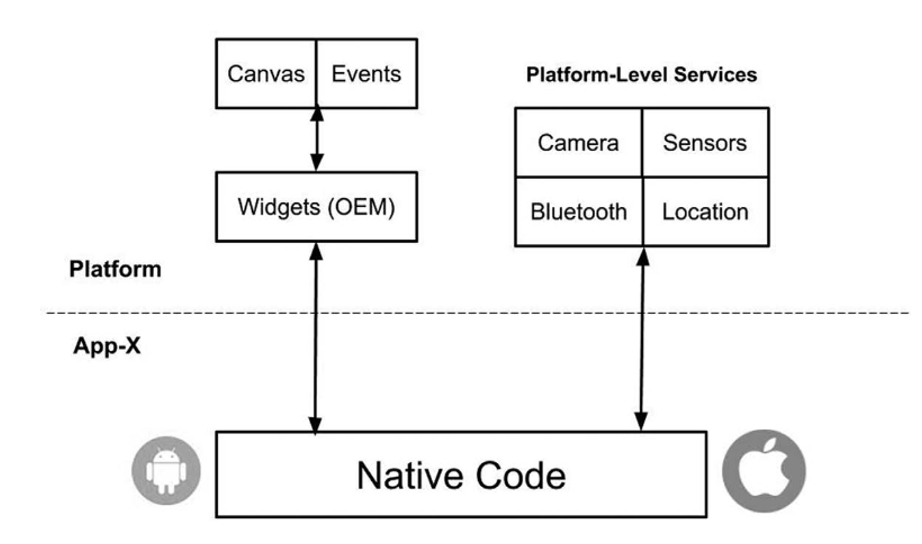
\includegraphics[width=15cm,height=8cm]{Images/system/flutter_native_code.png}
  \caption[Kiến trúc ứng dụng của hệ thống gốc]{\bfseries \fontsize{12pt}{0pt}
  \selectfont Kiến trúc ứng dụng của hệ thống gốc}
  \label{flutter_native_code} %đặt tên cho ảnh
\end{figure}

Hình ảnh trên thể hiện sự tương tác giữa Native Code và các dịch vụ của Platform một cách trực tiếp, nói cách khác, sử dụng
native code chúng ta có thể truy cập đến mọi services một cách nhanh chóng và thuận tiện nhất. Tuy nhiên việc thực hiện
code trên native cũng tương đối khó và đòi hỏi kinh nghiệm vì cấu trúc phức tạp và có hiểu biết về hệ điều hành.

\begin{figure}[H]
  \centering
  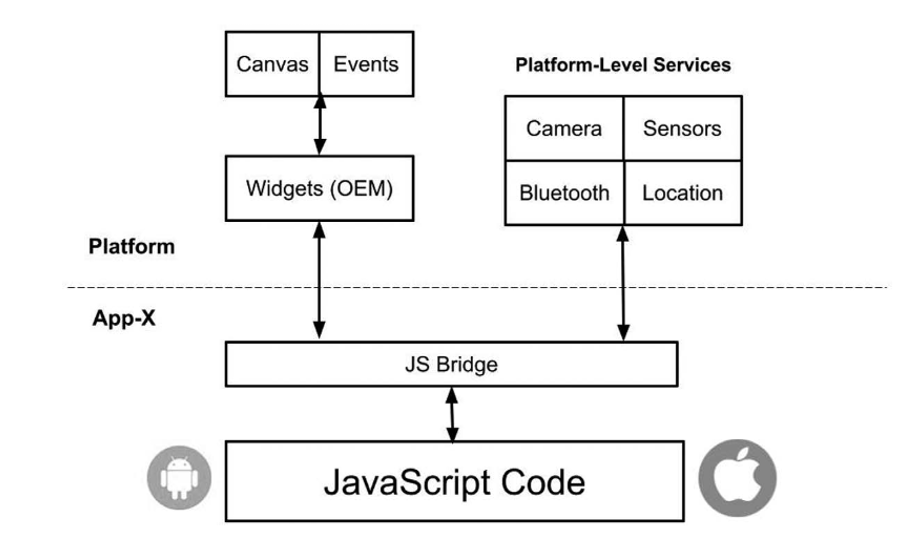
\includegraphics[width=15cm,height=8cm]{Images/system/flutter_JS.png}
  \caption[Kiến trúc ứng dụng của hệ thống sử dụng cầu nối Javascript]{\bfseries \fontsize{12pt}{0pt}
  \selectfont Kiến trúc ứng dụng của hệ thống sử dụng cầu nối Javascript}
  \label{flutter_JS} %đặt tên cho ảnh
\end{figure}

Tiếp theo, để xử lý những vấn đề gặp phải ở trên, giải pháp ở đây đó chính là sử dụng một cầu nối, cầu nối Javascript (một ngôn ngữ lập trình bậc cao)
sẽ giảm tải việc không phải chạm đến native code, đơn giản hoá việc code ứng dụng, nhược điểm là tốc độ xử lý và chạy ứng
dụng sẽ chậm hơn vì phải chuyển từ Javascript qua Native Code khi chạy. 

\begin{figure}[H]
  \centering
  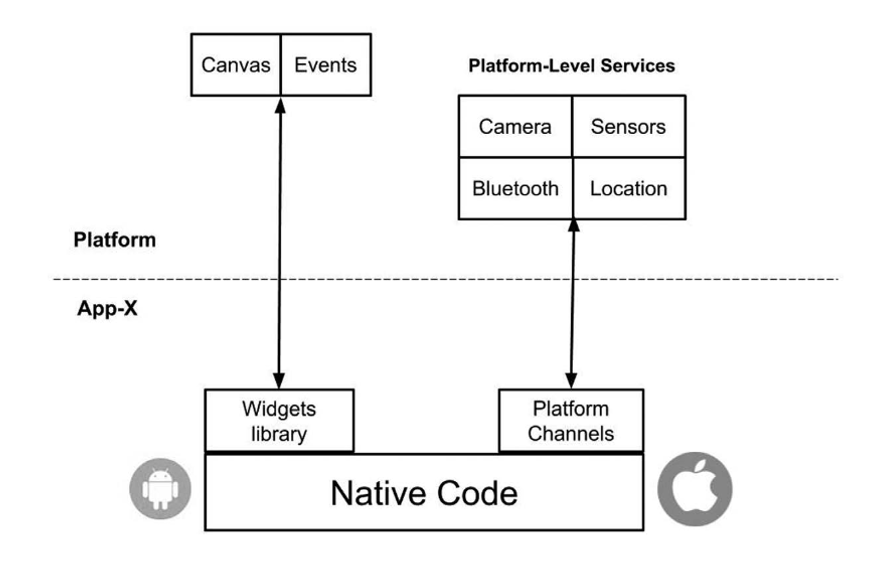
\includegraphics[width=15cm,height=8cm]{Images/system/flutter_dart.png}
  \caption[Kiến trúc ứng dụng của hệ thống sử dụng Method Channel Flutter]{\bfseries \fontsize{12pt}{0pt}
  \selectfont Kiến trúc ứng dụng của hệ thống sử dụng Method Channel Flutter}
  \label{flutter_dart} %đặt tên cho ảnh
\end{figure}

Giải pháp của Flutter là việc xây dựng sẵn Widget tương tác trực tiếp với Native Code, người dùng chỉ cần gọi Widget và tuỳ
biến dựa trên mong muốn, và Method Channel cho việc phát triển những chức năng mà Flutter chưa thực sự hỗ trợ. Việc kết hợp này
giúp cho tốc độ xử lý nhanh và đảm bảo có chiều sâu khi hỗ trợ cả Native Code bắt kỳ khi nào chúng ta cần.


\paragraph{Firebase}
\mbox{}

Ứng dụng di động của bệnh nhân và bác sĩ sử dụng Firebase Firestore để lưu trữ tin nhắn và trong tương lai sẽ sử dụng Firebase
Messaging để gửi thông báo đến cho người nhận. Dưới đây là phần giới thiệu của chúng em về Firebase Firestore:

Firebase Firestore: là một cơ sở dữ liệu NoSQL của Firebase, cho phép bạn lưu trữ và đồng bộ dữ liệu trong thời gian thực giữa ứng dụng của bạn và cơ sở dữ liệu trên đám mây. Firestore được thiết kế để cung cấp hiệu suất cao, đáng tin cậy và dễ sử dụng cho việc lưu trữ và truy vấn dữ liệu.
Đặc điểm của Firebase Firestore bao gồm:
\begin{itemize} 
  \item Lưu trữ dữ liệu dưới dạng tài liệu (document) và bộ sưu tập (collection) có cấu trúc linh hoạt
  \item Hỗ trợ lắng nghe sự thay đổi dữ liệu trong thời gian thực thông qua tính năng "realtime updates"
  \item Được tích hợp sâu với các sản phẩm và dịch vụ khác của Firebase, như Firebase Authentication, Firebase Cloud Functions, và Firebase Cloud Messaging
  \item Có SDK hỗ trợ nhiều nền tảng, bao gồm Android, iOS, web và cả Flutter.
\end{itemize}

\paragraph{Bluetooth Low Energy}
\mbox{}

Ứng dụng di động của bệnh nhân sử dụng Bluetooth với công nghệ Bluetooth Low Energy để truyền/nhận dữ liệu giữa ứng dụng di
động với thiết bị IOT. BLE được thiết kế để tiết kiệm năng lượng và thích hợp cho các ứng dụng yêu cầu tiêu thụ điện năng thấp 
và phạm vi hoạt động ngắn, rất phù hợp với thiết bị điện tim cần truyền dữ liệu liên tục đến ứng dụng. Trong ứng dụng di động này, chúng
em sử dụng đến hai khái niệm thường dùng trong BLE đó là Service và Characteristic.


\begin{itemize} 
  \item Service: được định danh bằng UUID, dùng để định nghĩa một chức năng cụ thể của thiết bị
  \item Characteristic: được định danh bằng UUID, thuộc về một service nhất định và có thể thực hiện việc đọc, ghi cũng như lắng nghe
\end{itemize}

Việc thực hiện lắng nghe Characteristic và lấy dữ liệu ra là chìa khoá của Bluetooth trong ứng dụng lần này.
  \begin{figure}[H]
        \centering
        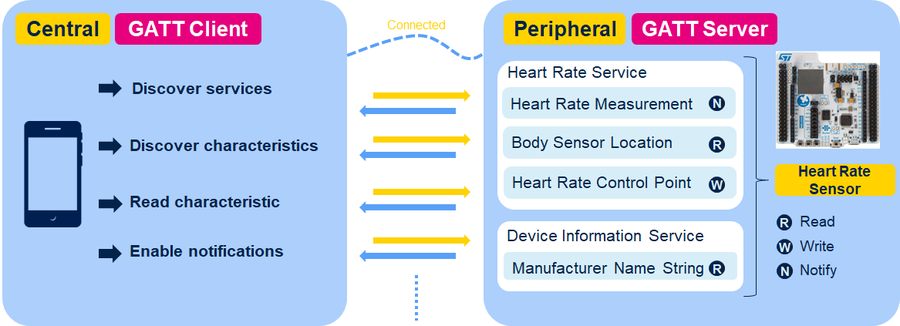
\includegraphics[width=16cm,height=8cm]{Images/system/ble_services.png}
        \caption[Ví dụ mô tả chức năng của Bluetooth Low Energy]{\bfseries \fontsize{12pt}{0pt}
        \selectfont Ví dụ mô tả chức năng của Bluetooth Low Energy}
        \label{ble_services} %đặt tên cho ảnh
  \end{figure}

  Hình \ref{ble_services} mô tả cách mà dữ liệu sẽ được truyền/nhận hay lắng nghe thông qua Write/Read/Notify. 
  Với Central (đại diện cho thiết bị di động), Peripheral đại diện cho thiết bị ngoại vi (thiết bị đo), sau khi kết nối giữa chúng 
  được thiết lập, việc giao tiếp giữa chúng phụ thuộc vào việc chúng ta sẽ kết nối với đúng UUID của từng services hay
  characteristic như đã được giới thiệu ở trên.

\subsubsection{Server và Website}

\paragraph{NodeJs}
\mbox{}

Node.js là một nền tảng phát triển ứng dụng mã nguồn mở cực kỳ mạnh mẽ và đa dạng, giúp các nhà phát triển xây dựng các ứng dụng web và dịch vụ server-side với hiệu suất cao và khả năng mở rộng linh hoạt. Được ra đời vào năm 2009, Node.js đã nhanh chóng trở thành một trong những công nghệ phổ biến nhất trong cộng đồng lập trình viên và được ứng dụng rộng rãi trong các dự án phức tạp cũng như các ứng dụng thời gian thực.

Một trong những điểm mạnh nổi bật của Node.js là sự hỗ trợ tốt cho kiến trúc không đồng bộ (asynchronous architecture). Bản chất của kiến trúc này là khả năng xử lý đa luồng (multithreading) không đồng bộ, giúp ứng dụng có thể xử lý nhiều yêu cầu cùng một lúc mà không phải chờ đợi hoàn thành từng yêu cầu trước. Điều này cho phép Node.js xử lý các yêu cầu I/O (Input/Output) nặng như truy vấn cơ sở dữ liệu, đọc/ghi dữ liệu từ tập tin, hay gửi và nhận các yêu cầu HTTP một cách hiệu quả và nhanh chóng. Sự không đồng bộ cũng giúp tăng hiệu suất cho ứng dụng, đồng thời tiết kiệm tài nguyên hệ thống.

Node.js được xây dựng dựa trên JavaScript, ngôn ngữ lập trình phổ biến và có tính linh hoạt cao. Sự hòa quyện giữa Node.js và JavaScript cho phép phát triển viên sử dụng cùng một ngôn ngữ cho cả phía client và phía server, giúp đơn giản hóa việc phát triển và duy trì mã nguồn. Ngoài ra, cộng đồng phát triển JavaScript rất lớn và đầy đủ tài nguyên học tập và hỗ trợ trực tuyến, điều này làm cho việc học và sử dụng Node.js trở nên dễ dàng và thuận tiện.

Vì Node.js là mã nguồn mở, nên nó rất linh hoạt và có khả năng tùy chỉnh cao. Phát triển viên có thể sửa đổi và mở rộng các tính năng của Node.js tùy theo nhu cầu của dự án một cách dễ dàng. Hơn nữa, Node.js có cộng đồng lớn và năng động, luôn cập nhật và cải tiến mã nguồn để đáp ứng yêu cầu của các dự án phức tạp và đa dạng. Cộng đồng Node.js cũng cung cấp rất nhiều các thư viện và module mở rộng, giúp tăng tính năng và hiệu suất của ứng dụng.

Một trong những ưu điểm nổi bật của Node.js là hỗ trợ đa nền tảng (cross-platform), cho phép chạy ứng dụng trên nhiều hệ điều hành khác nhau như Windows, macOS, Linux, và nhiều nền tảng khác. Điều này giúp đơn giản hóa quá trình triển khai và triển khai ứng dụng trên nhiều môi trường mà không cần thay đổi mã nguồn.

Một ưu điểm khác của Node.js là hỗ trợ tốt cho việc xây dựng các ứng dụng thời gian thực (real-time applications). Điều này rất hữu ích trong việc xây dựng các ứng dụng trò chơi trực tuyến, ứng dụng trò chuyện (chat applications), hay ứng dụng giao tiếp thời gian thực. Cơ chế WebSocket được tích hợp sẵn trong Node.js giúp kết nối và truyền thông dữ liệu giữa server và client một cách liên tục và nhanh chóng.

Bên cạnh đó, Node.js cũng hỗ trợ các thư viện và giao thức mạng như HTTP, HTTPS, TCP, và UDP, cho phép phát triển viên xây dựng các ứng dụng mạng phức tạp và mạnh mẽ. Node.js cũng cung cấp khả năng tạo máy chủ đơn giản và hiệu quả, giúp xây dựng các ứng dụng web phức tạp với khả năng mở rộng linh hoạt.

Trong việc lưu trữ dữ liệu, Node.js hỗ trợ cơ chế xử lý dữ liệu không đồng bộ, giúp tối ưu hóa hiệu suất của ứng dụng trong việc truy xuất và lưu trữ dữ liệu vào cơ sở dữ liệu. Node.js cũng hỗ trợ các cơ sở dữ liệu phổ biến như MySQL, PostgreSQL, MongoDB, và Redis, cho phép phát triển viên lựa chọn cơ sở dữ liệu phù hợp với yêu cầu của dự án.

Ngoài ra, Node.js còn hỗ trợ các tiện ích cho việc phát triển ứng dụng như gỡ lỗi (debugging), kiểm thử (testing), và quản lý gói (package management) thông qua npm (Node Package Manager). Việc sử dụng các công cụ và thư viện này giúp đơn giản hóa việc phát triển và nâng cao chất lượng của mã nguồn.

Trong quá trình triển khai ứng dụng, Node.js hỗ trợ dễ dàng tích hợp với các công cụ triển khai (deployment tools) như Docker và Kubernetes, giúp đơn giản hóa quá trình triển khai và vận hành ứng dụng trên các môi trường khác nhau.

Tổng kết lại, Node.js là một nền tảng phát triển ứng dụng đa dạng và mạnh mẽ, với nhiều ưu điểm nổi trội như kiến trúc không đồng bộ, tích hợp với JavaScript, đa nền tảng, hỗ trợ ứng dụng thời gian thực, và cộng đồng lớn hỗ trợ phong phú. Với những lợi ích đáng kể này, Node.js đã trở thành một lựa chọn ưu việt cho việc xây dựng các ứng dụng web và dịch vụ server-side hiệu quả và mạnh mẽ.

\paragraph{Javascript}
\mbox{}

JavaScript là một ngôn ngữ lập trình thông dịch, đa mục đích và được sử dụng phổ biến trên web. Nó ra đời vào năm 1995 bởi Brendan Eich, khi còn là một ngôn ngữ lập trình đơn giản để cung cấp tính năng tương tác và hiệu ứng động cho trang web. Tuy nhiên, từ đó đến nay, JavaScript đã trở thành một trong những ngôn ngữ lập trình quan trọng nhất trên thế giới, vượt qua giới hạn trang web và mở rộng sang nhiều lĩnh vực phát triển phần mềm khác nhau.

Một trong những yếu tố quan trọng đóng góp vào sự phổ biến của JavaScript là việc nó được tích hợp một cách tự nhiên và mạnh mẽ với các trình duyệt web. Trước khi JavaScript xuất hiện, việc tạo ra hiệu ứng động và tương tác trên trang web đòi hỏi sự hỗ trợ của các ngôn ngữ lập trình phía server như PHP hoặc các công nghệ khác. JavaScript đã định hình lại cách các ứng dụng web tương tác và hiển thị nội dung, giúp chúng trở nên đa dạng và mạnh mẽ hơn.

JavaScript là một ngôn ngữ linh hoạt và dễ tiếp cận, cho phép người phát triển xây dựng các ứng dụng phong phú và phức tạp với giao diện tương tác, kiểu dáng đẹp mắt và tính năng đa dạng. Ngôn ngữ này hỗ trợ một loạt các kiểu dữ liệu như số, chuỗi, mảng, đối tượng và hỗ trợ xử lý chuỗi, số học, ngày tháng, và các phép tính logic phức tạp.

Một điểm mạnh của JavaScript là khả năng xử lý các sự kiện (event) và gắn kết chúng vào các thành phần trên trang web. Sự kiện là những hành động như nhấp chuột, nhập liệu từ bàn phím, hoặc thay đổi trạng thái của trang web. JavaScript cho phép người phát triển xử lý các sự kiện này và thay đổi nội dung hoặc hành vi của trang web một cách linh hoạt, đáp ứng tương tác của người dùng.

Ngoài ra, JavaScript còn hỗ trợ các khái niệm cấu trúc dữ liệu và kiểu dữ liệu linh hoạt như đối tượng (object), mảng (array), và chuỗi (string). Điều này cho phép người phát triển xây dựng các ứng dụng phức tạp và có tính mô đun cao, giúp quản lý mã nguồn dễ dàng và giảm thiểu lỗi trong quá trình phát triển.

Một trong những tính năng đáng chú ý của JavaScript là khả năng thực hiện các yêu cầu mạng bất đồng bộ (asynchronous) thông qua việc sử dụng các API như XMLHttpRequest (XHR) hay Fetch API. Điều này cho phép trang web tương tác với các dịch vụ web và cơ sở dữ liệu một cách hiệu quả mà không làm trì hoãn trình duyệt.

JavaScript cũng hỗ trợ việc tạo ra các ứng dụng web động, đặc biệt là những ứng dụng đơn trang (single-page applications - SPA). SPA là mô hình phát triển ứng dụng web mà trang web chỉ tải một lần duy nhất khi người dùng truy cập, và sau đó các tương tác tiếp theo được thực hiện một cách bất đồng bộ thông qua JavaScript để cập nhật nội dung và thay đổi giao diện mà không cần tải lại trang. Điều này giúp tăng tốc độ và trải nghiệm người dùng.

Một yếu tố quan trọng khác là cộng đồng JavaScript rất đông đảo và nhiệt tình. Có rất nhiều người dùng và nhà phát triển trên toàn thế giới đóng góp và chia sẻ mã nguồn, thư viện, framework và các tài liệu học tập trực tuyến. Điều này làm cho việc học và sử dụng JavaScript trở nên dễ dàng và thuận tiện, đồng thời giúp phát triển viên giải quyết các vấn đề và thách thức trong quá trình xây dựng ứng dụng.

Một trong những hướng phát triển quan trọng của JavaScript là sự phát triển của các framework và thư viện mã nguồn mở như React, Angular, và Vue.js. Các framework này giúp người phát triển xây dựng các ứng dụng web phức tạp và mạnh mẽ một cách dễ dàng và hiệu quả hơn, đồng thời đảm bảo tính tương thích và bảo mật.

Tuy nhiên, JavaScript cũng có một số hạn chế như việc thực hiện mã nguồn phức tạp có thể dẫn đến các vấn đề bảo mật và hiệu suất. Để giải quyết vấn đề này, người phát triển cần phải tuân thủ các nguyên tắc phát triển an toàn và tối ưu hóa mã nguồn.

Tổng kết lại, JavaScript là một ngôn ngữ lập trình linh hoạt, mạnh mẽ và phổ biến, có nhiều ưu điểm vượt trội như tích hợp tốt với trình duyệt, đa dạng kiểu dữ liệu, khả năng thực hiện bất đồng bộ, và cộng đồng phát triển mạnh mẽ. JavaScript đã định hình lại cách các ứng dụng web tương tác và được sử dụng rộng rãi trong nhiều lĩnh vực phát triển phần mềm. Sự phát triển của các framework và thư viện JavaScript giúp người phát triển xây dựng các ứng dụng web phức tạp và mạnh mẽ một cách dễ dàng và hiệu quả hơn.

\paragraph{AdminJS}
\mbox{}

AdminJS là một framework mã nguồn mở được thiết kế để hỗ trợ phát triển các trang quản lý (admin dashboard) dễ dàng và nhanh chóng. Với AdminJS, người phát triển có thể xây dựng các giao diện quản lý phức tạp và mạnh mẽ một cách dễ dàng và hiệu quả, giúp quản lý và điều hành hệ thống, ứng dụng hoặc dịch vụ một cách thuận tiện và hiệu quả hơn.

Một trong những ưu điểm nổi bật của AdminJS là tích hợp các tính năng và chức năng phong phú sẵn có, giúp giảm thiểu thời gian và công sức trong việc xây dựng giao diện quản lý. AdminJS cung cấp các thành phần giao diện (UI components) sẵn có cho việc quản lý các bảng dữ liệu (data tables), hiển thị các biểu đồ thống kê, tạo các biểu mẫu nhập liệu (form fields) và nhiều tính năng khác. Nhờ vậy, người phát triển không cần phải viết mã nguồn từ đầu mà vẫn có thể xây dựng các trang quản lý đẹp mắt và chuyên nghiệp.

AdminJS hỗ trợ tích hợp với nhiều loại cơ sở dữ liệu phổ biến như MongoDB, PostgreSQL, MySQL, và SQLite, giúp tương tác và quản lý dữ liệu một cách dễ dàng. Ngoài ra, nó cũng hỗ trợ tích hợp với các framework và thư viện phổ biến như Express.js, Nest.js, và các thư viện mã nguồn mở khác. Tích hợp với các công nghệ này giúp AdminJS trở nên linh hoạt và dễ dàng tích hợp vào các dự án sẵn có.

Một tính năng quan trọng của AdminJS là khả năng tùy chỉnh và mở rộng. Người phát triển có thể tùy chỉnh các thành phần giao diện sẵn có để phù hợp với yêu cầu và phong cách của dự án. Điều này giúp tạo ra các trang quản lý có giao diện độc đáo và phù hợp với thương hiệu của dự án. Ngoài ra, người phát triển cũng có thể mở rộng và thêm các tính năng tùy chỉnh theo yêu cầu của dự án một cách dễ dàng.

AdminJS cũng hỗ trợ tích hợp các tính năng bảo mật và xác thực. Người phát triển có thể dễ dàng thiết lập và quản lý các quyền truy cập và vai trò người dùng trên các trang quản lý. Điều này giúp bảo mật và bảo vệ dữ liệu quan trọng khỏi việc truy cập trái phép. AdminJS cũng hỗ trợ tích hợp với các công nghệ bảo mật như JSON Web Token (JWT), Passport.js và các cơ chế xác thực khác.

Một điểm mạnh nữa của AdminJS là sự hỗ trợ mạnh mẽ từ cộng đồng. AdminJS có một cộng đồng đông đảo và năng động, luôn cập nhật và đóng góp cho mã nguồn để nâng cao tính năng và hiệu suất của framework. Cộng đồng cũng cung cấp rất nhiều tài liệu học tập và hỗ trợ trực tuyến, giúp người phát triển học hỏi và giải quyết các vấn đề trong quá trình xây dựng giao diện quản lý.

Ngoài ra, AdminJS còn hỗ trợ tích hợp với các công cụ phát triển phổ biến như VSCode, Sublime Text, và Atom, giúp tăng cường trải nghiệm phát triển và giảm thiểu lỗi trong quá trình phát triển. Nó cũng hỗ trợ tích hợp với các công cụ quản lý mã nguồn như Git và GitHub, giúp quản lý và kiểm soát phiên bản mã nguồn một cách hiệu quả.

Tóm lại, AdminJS là một framework mạnh mẽ và linh hoạt để xây dựng các trang quản lý (admin dashboard) dễ dàng và nhanh chóng. Với các tính năng và chức năng phong phú, tích hợp dễ dàng với nhiều loại cơ sở dữ liệu và khả năng tùy chỉnh mạnh mẽ, AdminJS giúp người phát triển xây dựng các giao diện quản lý chuyên nghiệp và mạnh mẽ một cách dễ dàng và hiệu quả. Sự hỗ trợ mạnh mẽ từ cộng đồng và tích hợp với các công cụ phát triển giúp tăng cường trải nghiệm phát triển và đảm bảo chất lượng của mã nguồn.

\paragraph{MySQL}
\mbox{}

MySQL là một hệ quản trị cơ sở dữ liệu mã nguồn mở phổ biến và mạnh mẽ, được sử dụng rộng rãi trong nhiều ứng dụng và dự án phát triển phần mềm. MySQL ra đời vào năm 1995, do công ty TcX phát triển và sau đó được mua lại bởi công ty MySQL AB. Hiện nay, MySQL thuộc sở hữu của Oracle Corporation sau khi Oracle mua lại Sun Microsystems - công ty mẹ của MySQL AB vào năm 2010.

MySQL là hệ quản trị cơ sở dữ liệu (DBMS - Database Management System) dựa trên mô hình quan hệ (relational database) và sử dụng ngôn ngữ truy vấn cấu trúc (Structured Query Language - SQL) để thực hiện các thao tác truy vấn dữ liệu. Mô hình quan hệ của MySQL cho phép lưu trữ và quản lý dữ liệu trong các bảng có mối quan hệ với nhau, tạo điều kiện để thực hiện các truy vấn phức tạp và hiệu quả.

MySQL hỗ trợ nhiều loại dữ liệu phổ biến như số, chuỗi, ngày tháng, boolean, và các kiểu dữ liệu đặc biệt khác như JSON và các kiểu dữ liệu không gian (spatial data types). Điều này giúp người dùng lưu trữ và xử lý các loại dữ liệu khác nhau một cách linh hoạt và hiệu quả.

Một trong những ưu điểm quan trọng của MySQL là hiệu suất cao và khả năng mở rộng linh hoạt. MySQL được tối ưu hóa để xử lý các yêu cầu truy vấn nhanh chóng và hiệu quả, cho phép xử lý hàng triệu hoặc thậm chí hàng tỷ bản ghi một cách mượt mà. Ngoài ra, MySQL cũng hỗ trợ tính năng phân chia dữ liệu (sharding) và nhân bản dữ liệu (replication), giúp tăng khả năng chịu tải và đảm bảo tính sẵn sàng và tin cậy của hệ thống.

MySQL cung cấp các tính năng bảo mật và quản lý người dùng mạnh mẽ. Người quản trị có thể xác định và quản lý các quyền truy cập của người dùng và vai trò của họ trên các bảng và cơ sở dữ liệu. Điều này giúp bảo vệ dữ liệu quan trọng và ngăn chặn truy cập trái phép.

MySQL hỗ trợ các công cụ và giao thức mạng như JDBC, ODBC, và các API kết nối khác, cho phép ứng dụng kết nối và tương tác với cơ sở dữ liệu MySQL từ các ứng dụng phần mềm và trang web khác nhau. MySQL cũng hỗ trợ giao thức kết nối và truy vấn an toàn, giúp đảm bảo tính bảo mật và chống lại các cuộc tấn công từ xa.

MySQL có sự hỗ trợ mạnh mẽ từ cộng đồng và cung cấp rất nhiều tài liệu học tập và hỗ trợ trực tuyến. Cộng đồng MySQL rất đông đảo và năng động, luôn cập nhật và đóng góp cho mã nguồn để nâng cao tính năng và hiệu suất của hệ quản trị cơ sở dữ liệu này.

MySQL cũng hỗ trợ tích hợp với các công cụ phát triển và quản lý mã nguồn như MySQL Workbench, phpMyAdmin và các công cụ khác, giúp quản lý và xem xét dữ liệu một cách thuận tiện và hiệu quả.

Một điểm đáng chú ý nữa của MySQL là tính tương thích với nhiều hệ điều hành và nền tảng khác nhau. MySQL có phiên bản dành cho Windows, macOS và các hệ điều hành Linux khác nhau, giúp người dùng lựa chọn và triển khai phù hợp với môi trường họ sử dụng.

Tóm lại, MySQL là một hệ quản trị cơ sở dữ liệu mã nguồn mở mạnh mẽ và phổ biến, được sử dụng rộng rãi trong nhiều ứng dụng và dự án phát triển phần mềm. Với tính năng hiệu suất cao, khả năng mở rộng linh hoạt, tính bảo mật và quản lý người dùng, sự hỗ trợ từ cộng đồng và tích hợp với nhiều công cụ phát triển, MySQL đã trở thành một lựa chọn ưu việt cho việc quản lý và xử lý cơ sở dữ liệu.


\paragraph{Postman}
\mbox{}

Postman là một ứng dụng máy tính được sử dụng phổ biến trong quá trình phát triển và kiểm thử các dịch vụ web (web service) và các API (Application Programming Interface). Được phát triển bởi công ty Postman Inc., ứng dụng này cung cấp một giao diện đơn giản và dễ sử dụng để gửi các yêu cầu HTTP (HTTP request) và nhận các phản hồi (response) từ các API. Postman giúp người phát triển dễ dàng thử nghiệm và kiểm tra tính năng, hiệu năng và bảo mật của các dịch vụ web và API, từ đó đảm bảo chất lượng và độ tin cậy của ứng dụng.

Một trong những ưu điểm nổi bật của Postman là khả năng gửi các yêu cầu HTTP một cách linh hoạt và dễ dàng. Người dùng có thể tùy chỉnh các yêu cầu HTTP bằng cách thêm các thông số và tham số, cũng như xác định các phương thức HTTP như GET, POST, PUT, DELETE, và nhiều phương thức khác. Điều này giúp người phát triển kiểm tra các chức năng khác nhau của API và dịch vụ web một cách hiệu quả.

Postman cũng hỗ trợ quản lý các môi trường (environments) khác nhau, cho phép người dùng cấu hình các giá trị môi trường như URL, token xác thực, hay các giá trị động khác. Nhờ vậy, người dùng có thể thử nghiệm các yêu cầu API trên nhiều môi trường khác nhau một cách dễ dàng, từ đó giả lập các trường hợp sử dụng và kiểm tra tính ổn định của API.

Một tính năng mạnh mẽ khác của Postman là khả năng tự động hóa các bước kiểm thử và thực hiện các bộ kiểm thử (test suite). Người dùng có thể viết các mã kiểm thử (test script) bằng ngôn ngữ JavaScript để kiểm tra phản hồi từ API và đánh giá tính đúng đắn của dữ liệu trả về. Điều này giúp tăng cường tính tin cậy của các bài kiểm thử và giảm thiểu nguy cơ sai sót từ phía người dùng.

Postman hỗ trợ tích hợp với các công cụ và dịch vụ phổ biến khác như GitHub, Jenkins, và các công cụ kiểm thử liên quan khác. Điều này giúp người phát triển tích hợp Postman vào quy trình phát triển phần mềm tự động một cách dễ dàng, từ việc kiểm tra mã nguồn đến việc chạy các bài kiểm thử tự động.

Postman cung cấp giao diện người dùng thân thiện và trực quan, giúp người dùng dễ dàng thao tác và nắm bắt các tính năng của ứng dụng. Nó cũng hỗ trợ nhiều loại dữ liệu và định dạng như JSON, XML, và form data, giúp người dùng kiểm thử các yêu cầu API đa dạng và phong phú.

Ngoài ra, Postman còn hỗ trợ tích hợp với Postman Cloud, một dịch vụ lưu trữ dữ liệu trực tuyến cho phép người dùng chia sẻ và quản lý các bài kiểm thử và dữ liệu API trực tuyến. Điều này giúp tăng cường sự cộng tác và quản lý dự án trong quá trình phát triển.

Postman đã trở thành một công cụ quan trọng và không thể thiếu trong quá trình phát triển và kiểm thử các ứng dụng và dịch vụ web. Sự dễ dàng sử dụng, tích hợp và tự động hóa giúp tăng cường năng suất và chất lượng của quá trình phát triển, đồng thời giảm thiểu nguy cơ lỗi và tối ưu hóa hiệu suất của ứng dụng.


\subsection{Thiết kế cơ sở dữ liệu}


\subsubsection{Chuyển mô hình thực thể liên kết sang mô hình quan hệ}

\begin{itemize}
  \item Người dùng (\textbf{ID người dùng}, Mật khẩu, Email, Tên, Ngày sinh, Số điện thoại, Quyền)
  \item Bản ghi ECG (\textbf{ID bản ghi ECG}, ID người dùng, ID thiết bị, Đường dẫn lưu trữ dữ liệu, Thời gian bắt đầu đo, Thời gian kết thúc đo, Loại cảm biến)
  \item Danh mục tin tức (\textbf{ID danh mục tin tức}, Tên danh mục tin tức, Mô tả danh mục tin tức)
  \item Tin tức (\textbf{ID tin tức}, Tiêu đề, Nội dung, ID danh mục tin tức, Tác giả, Đường dẫn, Đường dẫn hình ảnh)
  \item Phân công bệnh nhân - bác sĩ (\textbf{ID phân công}, ID bệnh nhân, ID bác sĩ, Ngày bắt đầu)
  \item Mã thông báo đặt lại mật khẩu (\textbf{ID mã thông báo}, ID người dùng, Mã thông báo, Thời gian hết hạn)
  \item Phiên đăng nhập (\textbf{ID phiên đăng nhập}, ID người dùng, Mã phiên đăng nhập, Thời gian hết hạn)
  \item Thiết bị (\textbf{ID thiết bị}, Tên thiết bị)
\end{itemize}



\subsubsection{Mối quan hệ dữ liệu}

\begin{itemize}
  \item Bảng \texttt{ecg\_record} có mối quan hệ 1-n với bảng \texttt{user} thông qua khóa ngoại \texttt{user\_id}.
  \item Bảng \texttt{news} có mối quan hệ n-1 với bảng \texttt{news\_category} thông qua khóa ngoại \texttt{category\_id}.
  \item Bảng \texttt{patient\_doctor\_assignment} có mối quan hệ n-1 với bảng \texttt{user} thông qua khóa ngoại \texttt{patient\_id} và \texttt{doctor\_id}.
  \item Bảng \texttt{reset\_token} có mối quan hệ n-1 với bảng \texttt{user} thông qua khóa ngoại \texttt{user\_id}.
\end{itemize}

\subsubsection{Chuẩn hoá 3NF}
Các bảng đã được thiết kế theo nguyên tắc chuẩn hoá 3NF, vì không có thuộc tính lặp lại và các thuộc tính không phụ thuộc vào một tập hợp con của khóa chính.

\paragraph{Chuẩn hoá bảng Người dùng}
\mbox{}

\begin{table}[H]
  \caption{\bfseries \fontsize{12pt}{0pt}\selectfont Bảng chuẩn hoá bảng Người dùng}
  \centering
  \begin{tabularx}{0.9\textwidth}{|X|X|}
    \hline
    \textbf{Danh sách thuộc tính} & ID người dùng, Mật khẩu, Email, Tên, Ngày sinh, Số điện thoại,
    Quyền \\ % Thêm \textbf{} cho abc
    \hline
    \textbf{Quy tắc nghiệp vụ} & \textbf{Phụ thuộc hàm} \\
    \hline
    Mỗi người dùng có một ID riêng, có duy nhất mật khẩu, email, tên, ngày sinh, số điện thoại,
    quyền & \parbox[t]{\linewidth}{$\text{ID người dùng} \rightarrow$ mật khẩu, email, tên, ngày sinh, số điện thoại, quyền} \\
    \hline
    \multicolumn{2}{|X|}{$\Rightarrow \text{Khoá chính của bảng: ID người dùng}$} \\
    \multicolumn{2}{|X|}{$\Rightarrow \text{Bảng Người dùng đã ở 3NF}$} \\
    \hline
  \end{tabularx}
\end{table}


\paragraph{Chuẩn hoá bảng Bản ghi ECG}
\mbox{}

\begin{table}[H]
  \caption{\bfseries \fontsize{12pt}{0pt}\selectfont Bảng chuẩn hoá bảng Bản ghi ECG}
  \centering
  \begin{tabularx}{0.9\textwidth}{|X|X|}
    \hline
    \textbf{Danh sách thuộc tính} & ID bản ghi ECG, ID người dùng, ID thiết bị, Đường dẫn lưu trữ dữ
    liệu, Thời gian bắt đầu đo, Thời gian kết thúc đo, Loại cảm biến \\
    \hline
    \textbf{Quy tắc nghiệp vụ} & \textbf{Phụ thuộc hàm} \\
    \hline
    Mỗi bản ghi ECG có một ID riêng, có duy nhất ID người dùng, ID thiết bị, đường dẫn lưu trữ dữ
    liệu, thời gian bắt đầu đo, thời gian kết thúc đo, loại cảm biến & \parbox[t]{\linewidth}{$ \text{ID bản ghi ECG} \rightarrow$ ID người dùng, ID thiết bị, đường dẫn lưu trữ dữ
    liệu, thời gian bắt đầu đo, thời gian kết thúc đo, loại cảm biến} \\
    \hline
    \multicolumn{2}{|X|}{$\Rightarrow \text{Khoá chính của bảng: ID bản ghi ECG}$} \\
    \multicolumn{2}{|X|}{$\Rightarrow \text{Bảng Bản ghi ECG đã ở 3NF}$} \\
    \hline
  \end{tabularx}
\end{table}


\paragraph{Chuẩn hoá bảng Danh mục tin tức}
\mbox{}


\begin{table}[H]
  \caption{\bfseries \fontsize{12pt}{0pt}\selectfont Bảng chuẩn hoá bảng Danh mục tin tức}
  \centering
  \begin{tabularx}{0.9\textwidth}{|X|X|}
    \hline
    \textbf{Danh sách thuộc tính} & ID danh mục tin tức, Tên danh mục tin tức, Mô tả danh mục tin
    tức \\ % Thêm \textbf{} cho abc
    \hline
    \textbf{Quy tắc nghiệp vụ} & \textbf{Phụ thuộc hàm} \\
    \hline
    Mỗi danh mục tin tức có một ID riêng, có duy nhất tên danh mục tin tức, mô tả danh mục tin
    tức & \parbox[t]{\linewidth}{$\text{ID danh mục tin tức} \rightarrow$ danh mục tin tức, mô tả danh mục tin
    tức} \\
    \hline
    \multicolumn{2}{|X|}{$\Rightarrow \text{Khoá chính của bảng: ID danh mục tin tức}$} \\
    \multicolumn{2}{|X|}{$\Rightarrow \text{Bảng Danh mục tin tức đã ở 3NF}$} \\
    \hline
  \end{tabularx}
\end{table}


\paragraph{Chuẩn hoá bảng Tin tức}
\mbox{}

\begin{table}[H]
  \caption{\bfseries \fontsize{12pt}{0pt}\selectfont Bảng chuẩn hoá bảng Tin tức}
  \centering
  \begin{tabularx}{0.9\textwidth}{|X|X|}
    \hline
    \textbf{Danh sách thuộc tính} & ID tin tức, Tiêu đề, Nội dung, ID danh mục tin tức, Tác giả, Đường dẫn,
    Đường dẫn hình ảnh \\ % Thêm \textbf{} cho abc
    \hline
    \textbf{Quy tắc nghiệp vụ} & \textbf{Phụ thuộc hàm} \\
    \hline
    Mỗi tin tức có một ID riêng, có duy nhất tiêu đề, nội dung, ID danh mục tin tức, tác giả, đường dẫn,
    đường dẫn hình ảnh & \parbox[t]{\linewidth}{$\text{ID tin tức} \rightarrow$ tiêu đề, nội dung, ID danh mục tin tức, tác giả, đường dẫn,
    đường dẫn hình ảnh} \\
    \hline
    \multicolumn{2}{|X|}{$\Rightarrow \text{Khoá chính của bảng: ID tin tức}$} \\
    \multicolumn{2}{|X|}{$\Rightarrow \text{Bảng Tin tức đã ở 3NF}$} \\
    \hline
  \end{tabularx}
\end{table}



\paragraph{Chuẩn hoá bảng Phân công bệnh nhân - bác sĩ}
\mbox{}

\begin{table}[H]
  \caption{\bfseries \fontsize{12pt}{0pt}\selectfont Bảng chuẩn hoá bảng Phân công bệnh nhân - bác sĩ}
  \centering
  \begin{tabularx}{0.9\textwidth}{|X|X|}
    \hline
    \textbf{Danh sách thuộc tính} & ID phân công, ID bệnh nhân, ID bác sĩ, Ngày bắt
    đầu \\ % Thêm \textbf{} cho abc
    \hline
    \textbf{Quy tắc nghiệp vụ} & \textbf{Phụ thuộc hàm} \\
    \hline
    Mỗi lần phân công bệnh nhân - bác sĩ có một ID riêng, có duy nhất ID bệnh nhân, ID bác sĩ, ngày bắt
    đầu & \parbox[t]{\linewidth}{$\text{ID phân công} \rightarrow$ ID bệnh nhân, ID bác sĩ, ngày bắt
    đầu} \\
    \hline
    \multicolumn{2}{|X|}{$\Rightarrow \text{Khoá chính của bảng: ID phân công}$} \\
    \multicolumn{2}{|X|}{$\Rightarrow \text{Bảng Phân công bệnh nhân - bác sĩ đã ở 3NF}$} \\
    \hline
  \end{tabularx}
\end{table}




\paragraph{Chuẩn hoá bảng Mã thông báo đặt lại mật khẩu}
\mbox{}

\begin{table}[H]
  \caption{\bfseries \fontsize{12pt}{0pt}\selectfont Bảng chuẩn hoá bảng Mã thông báo đặt lại mật khẩu}
  \centering
  \begin{tabularx}{0.9\textwidth}{|X|X|}
    \hline
    \textbf{Danh sách thuộc tính} & ID mã thông báo, ID người dùng, Mã thông báo,
    Thời gian hết hạn \\ % Thêm \textbf{} cho abc
    \hline
    \textbf{Quy tắc nghiệp vụ} & \textbf{Phụ thuộc hàm} \\
    \hline
    Mỗi mã thông báo đặt lại mật khẩu có một ID riêng, có duy nhất ID người dùng, mã thông báo,
    thời gian hết hạn & \parbox[t]{\linewidth}{$\text{ID mã thông báo} \rightarrow$ ID người dùng, mã thông báo,
    thời gian hết hạn} \\
    \hline
    \multicolumn{2}{|X|}{$\Rightarrow \text{Khoá chính của bảng: ID mã thông báo}$} \\
    \multicolumn{2}{|X|}{$\Rightarrow \text{Bảng Mã thông báo đặt lại mật khẩu đã ở 3NF}$} \\
    \hline
  \end{tabularx}
\end{table}


\paragraph{Chuẩn hoá bảng Phiên đăng nhập}
\mbox{}

\begin{table}[H]
  \caption{\bfseries \fontsize{12pt}{0pt}\selectfont Bảng chuẩn hoá bảng Phiên đăng nhập}
  \centering
  \begin{tabularx}{0.9\textwidth}{|X|X|}
    \hline
    \textbf{Danh sách thuộc tính} & ID phiên đăng nhập, ID người dùng, Mã phiên đăng nhập, Thời
    gian hết hạn \\ % Thêm \textbf{} cho abc
    \hline
    \textbf{Quy tắc nghiệp vụ} & \textbf{Phụ thuộc hàm} \\
    \hline
    Mỗi phiên đăng nhập có một ID riêng, có duy nhất ID người dùng, mã phiên đăng nhập, thời
    gian hết hạn & \parbox[t]{\linewidth}{$\text{ID phiên đăng nhập} \rightarrow$ ID người dùng, mã phiên đăng nhập, thời
    gian hết hạn} \\
    \hline
    \multicolumn{2}{|X|}{$\Rightarrow \text{Khoá chính của bảng: ID phiên đăng nhập}$} \\
    \multicolumn{2}{|X|}{$\Rightarrow \text{Bảng Phiên đăng nhập đã ở 3NF}$} \\
    \hline
  \end{tabularx}
\end{table}



\paragraph{Chuẩn hoá bảng Thiết bị}
\mbox{}

\begin{table}[H]
  \caption{\bfseries \fontsize{12pt}{0pt}\selectfont Bảng chuẩn hoá bảng Thiết bị}
  \centering
  \begin{tabularx}{0.9\textwidth}{|X|X|}
    \hline
    \textbf{Danh sách thuộc tính} & ID thiết bị, Tên thiết bị \\ % Thêm \textbf{} cho abc
    \hline
    \textbf{Quy tắc nghiệp vụ} & \textbf{Phụ thuộc hàm} \\
    \hline
    Mỗi thiết bị có một ID riêng, có duy nhất tên thiết bị & \parbox[t]{\linewidth}{$\text{ID thiết bị} \rightarrow$ tên thiết bị} \\
    \hline
    \multicolumn{2}{|X|}{$\Rightarrow \text{Khoá chính của bảng: ID thiết bị}$} \\
    \multicolumn{2}{|X|}{$\Rightarrow \text{Bảng Thiết bị đã ở 3NF}$} \\
    \hline
  \end{tabularx}
\end{table}




\subsubsection{Từ điển dữ liệu}



\begin{table}[H]
  \caption{\bfseries \fontsize{12pt}{0pt}\selectfont Bảng user}
  \centering
  \begin{tabularx}{0.9\textwidth}{|c|c|X|}
    \hline
    \textbf{Thuộc tính} & \textbf{Kiểu dữ liệu} & \textbf{Mô tả} \\
    \hline
    user\_id & INTEGER & Khóa chính của bảng, đại diện cho ID người dùng. \\
    \hline
    password & STRING & Mật khẩu của người dùng. \\
    \hline
    email & STRING & Địa chỉ email của người dùng. \\
    \hline
    name & STRING & Tên của người dùng. \\
    \hline
    doB & DATE & Ngày sinh của người dùng. \\
    \hline
    phone\_number & STRING & Số điện thoại của người dùng. \\
    \hline
    role & INTEGER & Quyền của người dùng (0-patient, 1-doctor, 2-admin). \\
    \hline
    created\_at & DATE & Thời điểm thêm mới dữ liệu vào database. \\
    \hline
    updated\_at & DATE & Thời điểm cập nhật dữ liệu vào database. \\
    \hline
    
  \end{tabularx}
\end{table}

\begin{table}[H]
  \caption{\bfseries \fontsize{12pt}{0pt}\selectfont Bảng ecg\_record}
  \centering
  \begin{tabularx}{0.9\textwidth}{|c|c|X|}
    \hline
    \textbf{Thuộc tính} & \textbf{Kiểu dữ liệu} & \textbf{Mô tả} \\
    \hline
    record\_id & INTEGER & Khóa chính của bảng, đại diện cho ID bản ghi ECG. \\
    \hline
    user\_id & INTEGER & Khóa ngoại tham chiếu đến \texttt{user\_id} trong bảng \texttt{user}. \\
    \hline
    device\_id & STRING & ID thiết bị. \\
    \hline
    data\_directory & STRING & Đường dẫn lưu trữ dữ liệu. \\
    \hline
    start\_time & DATE & Thời gian bắt đầu ghi lại ECG. \\
    \hline
    stop\_time & DATE & Thời gian kết thúc ghi lại ECG. \\
    \hline
    sensor\_type & STRING & Loại cảm biến. \\
    \hline
    created\_at & DATE & Thời điểm thêm mới dữ liệu vào database. \\
    \hline
    updated\_at & DATE & Thời điểm cập nhật dữ liệu vào database. \\
    \hline
  \end{tabularx}
\end{table}

\begin{table}[H]
  \caption{\bfseries \fontsize{12pt}{0pt}\selectfont Bảng news\_category}
  \centering
  \begin{tabularx}{0.9\textwidth}{|c|c|X|}
    \hline
    \textbf{Thuộc tính} & \textbf{Kiểu dữ liệu} & \textbf{Mô tả} \\
    \hline
    category\_id & INTEGER & Khóa chính của bảng, đại diện cho ID danh mục tin tức. \\
    \hline
    category\_name & STRING & Tên danh mục tin tức. \\
    \hline
    category\_description & STRING & Mô tả danh mục tin tức. \\
    \hline
    created\_at & DATE & Thời điểm thêm mới dữ liệu vào database. \\
    \hline
    updated\_at & DATE & Thời điểm cập nhật dữ liệu vào database. \\
    \hline
  \end{tabularx}
\end{table}

\begin{table}[H]
  \caption{\bfseries \fontsize{12pt}{0pt}\selectfont Bảng news}
  \centering
  \begin{tabularx}{0.9\textwidth}{|c|c|X|}
    \hline
    \textbf{Thuộc tính} & \textbf{Kiểu dữ liệu} & \textbf{Mô tả} \\
    \hline
    news\_id & INTEGER & Khóa chính của bảng, đại diện cho ID tin tức. \\
    \hline
    title & STRING & Tiêu đề tin tức. \\
    \hline
    content & TEXT & Nội dung tin tức. \\
    \hline
    category\_id & INTEGER & Khóa ngoại tham chiếu đến \texttt{category\_id} trong bảng \texttt{news\_category}. \\
    \hline
    author & STRING & Tác giả tin tức. \\
    \hline
    url & STRING & Đường dẫn tin tức. \\
    \hline
    image & STRING & Đường dẫn hình ảnh tin tức (có thể là null). \\
    \hline
    created\_at & DATE & Thời điểm thêm mới dữ liệu vào database. \\
    \hline
    updated\_at & DATE & Thời điểm cập nhật dữ liệu vào database. \\
    \hline
  \end{tabularx}
\end{table}

\begin{table}[H]
  \caption{\bfseries \fontsize{12pt}{0pt}\selectfont Bảng patient\_doctor\_assignment}
  \centering
  \begin{tabularx}{0.9\textwidth}{|c|c|X|}
    \hline
    \textbf{Thuộc tính} & \textbf{Kiểu dữ liệu} & \textbf{Mô tả} \\
    \hline
    assign\_id & INTEGER & Khóa chính của bảng, đại diện cho ID phân công bệnh nhân - bác sĩ. \\
    \hline
    patient\_id & INTEGER & Khóa ngoại tham chiếu đến \texttt{user\_id} trong bảng \texttt{user} (với quyền là bệnh nhân). \\
    \hline
    doctor\_id & INTEGER & Khóa ngoại tham chiếu đến \texttt{user\_id} trong bảng \texttt{user} (với quyền là bác sĩ). \\
    \hline
    start\_date & DATE & Ngày bắt đầu phân công. \\
    \hline
    created\_at & DATE & Thời điểm thêm mới dữ liệu vào database. \\
    \hline
    updated\_at & DATE & Thời điểm cập nhật dữ liệu vào database. \\
    \hline
  \end{tabularx}
\end{table}

\begin{table}[H]
  \caption{\bfseries \fontsize{12pt}{0pt}\selectfont Bảng reset\_token}
  \centering
  \begin{tabularx}{0.9\textwidth}{|c|c|X|}
    \hline
    \textbf{Thuộc tính} & \textbf{Kiểu dữ liệu} & \textbf{Mô tả} \\
    \hline
    id & INTEGER & Khóa chính của bảng, đại diện cho ID mã thông báo đặt lại. \\
    \hline
    user\_id & INTEGER & Khóa ngoại tham chiếu đến \texttt{user\_id} trong bảng \texttt{user}. \\
    \hline
    token & STRING & Mã thông báo đặt lại. \\
    \hline
    expiration & DATE & Thời gian hết hạn của mã thông báo đặt lại. \\
    \hline
    created\_at & DATE & Thời điểm thêm mới dữ liệu vào database. \\
    \hline
    updated\_at & DATE & Thời điểm cập nhật dữ liệu vào database. \\
    \hline
  \end{tabularx}
\end{table}


\begin{table}[H]
  \caption{\bfseries \fontsize{12pt}{0pt}\selectfont Bảng session}
  \centering
  \begin{tabularx}{0.9\textwidth}{|c|c|X|}
    \hline
    \textbf{Thuộc tính} & \textbf{Kiểu dữ liệu} & \textbf{Mô tả} \\
    \hline
    session\_id & INTEGER & Khóa chính của bảng, đại diện cho ID phiên đăng nhập. \\
    \hline
    user\_id & INTEGER & Khóa ngoại tham chiếu đến \texttt{user\_id} trong bảng \texttt{user}. \\
    \hline
    token & STRING & Mã phiên đăng nhập. \\
    \hline
    expiration & DATE & Thời gian hết hạn của phiên đăng nhập. \\
    \hline
    created\_at & DATE & Thời điểm thêm mới dữ liệu vào database. \\
    \hline
    updated\_at & DATE & Thời điểm cập nhật dữ liệu vào database. \\
    \hline
  \end{tabularx}
\end{table}

\begin{table}[H]
  \caption{\bfseries \fontsize{12pt}{0pt}\selectfont Bảng device}
  \centering
  \begin{tabularx}{0.9\textwidth}{|c|c|X|}
    \hline
    \textbf{Thuộc tính} & \textbf{Kiểu dữ liệu} & \textbf{Mô tả} \\
    \hline
    device\_id & INTEGER & Khóa chính của bảng, đại diện cho ID thiết bị. \\
    \hline
    device\_name & STRING & Tên thiết bị. \\
    \hline
    created\_at & DATE & Thời điểm thêm mới dữ liệu vào database. \\
    \hline
    updated\_at & DATE & Thời điểm cập nhật dữ liệu vào database. \\
    \hline
  \end{tabularx}
\end{table}

\subsubsection{Sơ đồ ERD}

\begin{figure}[H]
  \centering
  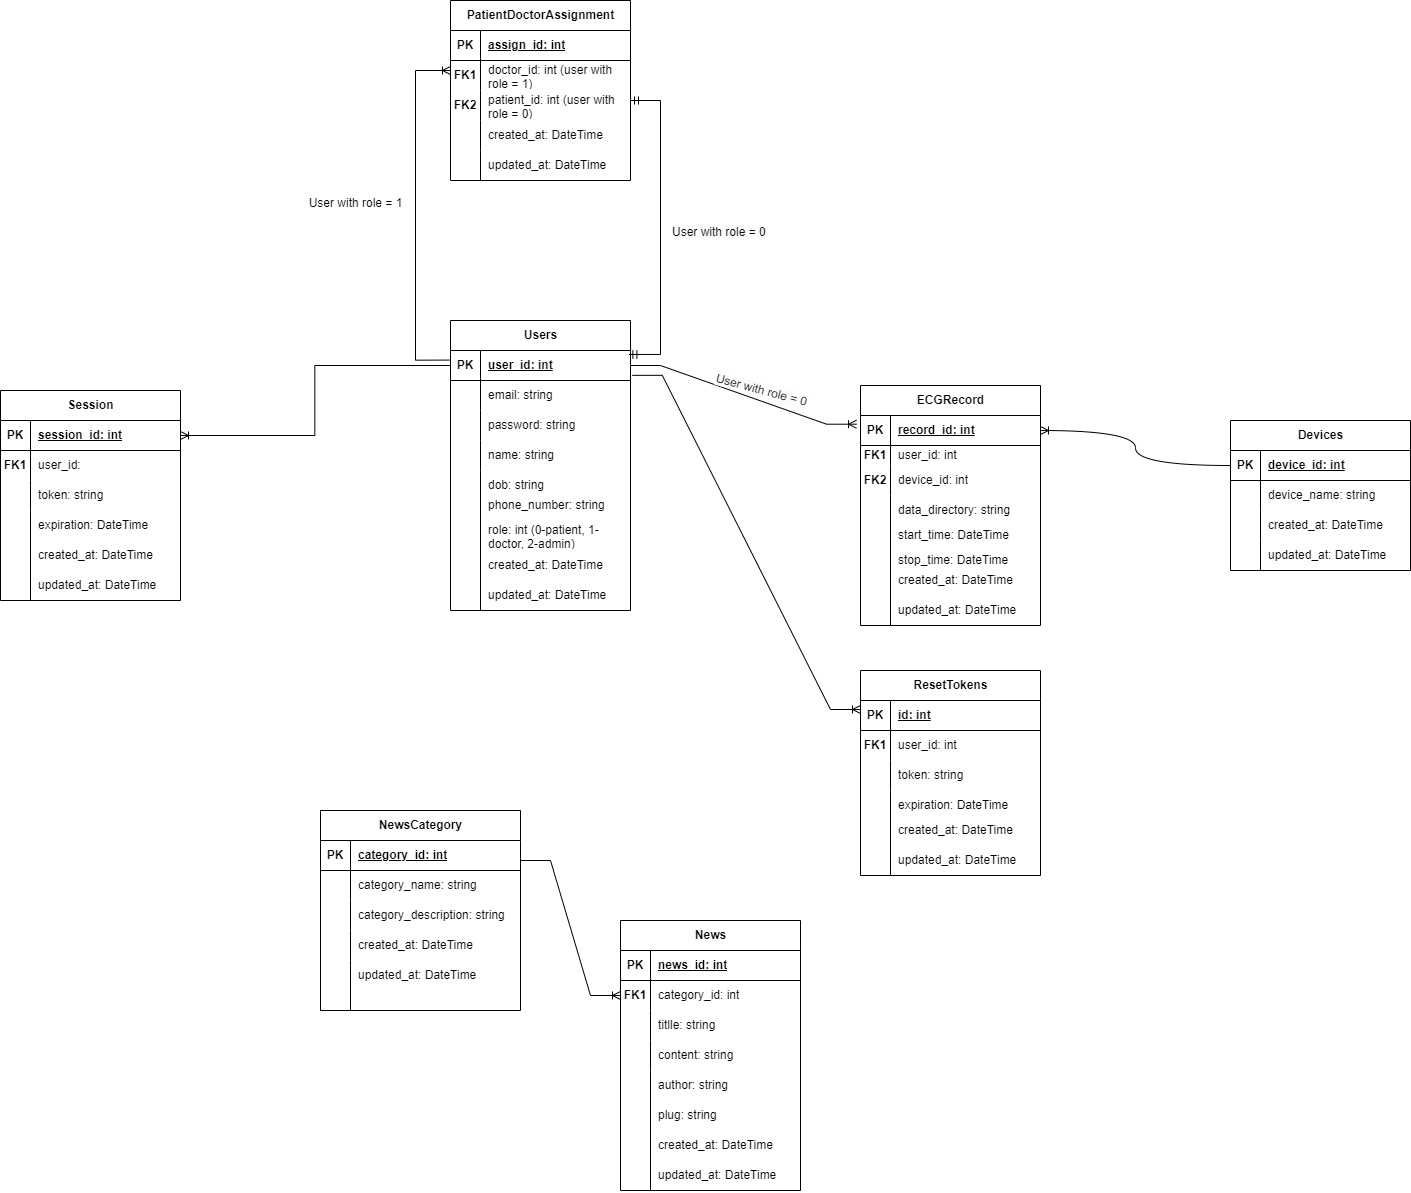
\includegraphics[width=15cm,height=15cm]{Images/server/database/fmECG_architecture-Database.drawio.png}
  \caption[Sơ đồ ERD]{\bfseries \fontsize{12pt}{0pt}\selectfont Sơ đồ ERD}
  \label{fmECG_architecture-Database} %đặt tên cho ảnh
\end{figure}




\subsection{Phân tích chi tiết hệ thống}

\subsubsection{Thiết kế giao diện}

\paragraph{Ứng dụng}
\mbox{}

Dưới đây là các giao diện thực tế mà chúng em thiết kế cho App:
\begin{figure}[H]
  \centering
  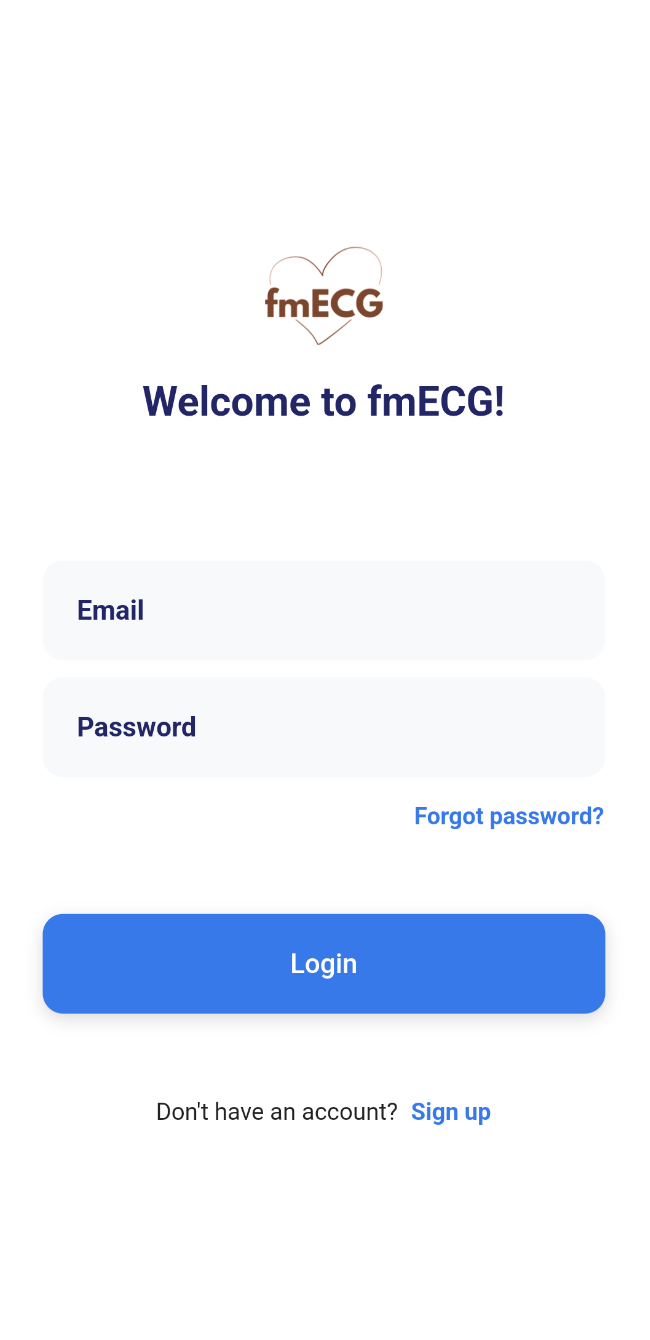
\includegraphics[width=6cm,height=12cm]{Images/mobile_app/demo/login.png}
  \caption[Giao diện trang đăng nhập]{\bfseries \fontsize{12pt}{0pt}\selectfont Giao diện trang đăng nhập}
  \label{demo_login} %đặt tên cho ảnh
\end{figure}

Trang đăng nhập gồm có logo, sau đó là hai ô để nhập email và mật khẩu, cùng một nút màu xanh cho người dùng nhấn để kiểm tra 
việc đăng nhập vào
trang chủ nếu email và mật khẩu của người dùng được xác thực. Nếu việc xác thực không thành công, giao diện sẽ hiển thị
một dòng chữ dưới hai ô nhập.

Ngoài ra nếu người dùng chưa có tài khoản thì có thể chọn đăng ký ở dưới để chuyển sang trang đăng ký.

\begin{figure}[H]
  \centering
  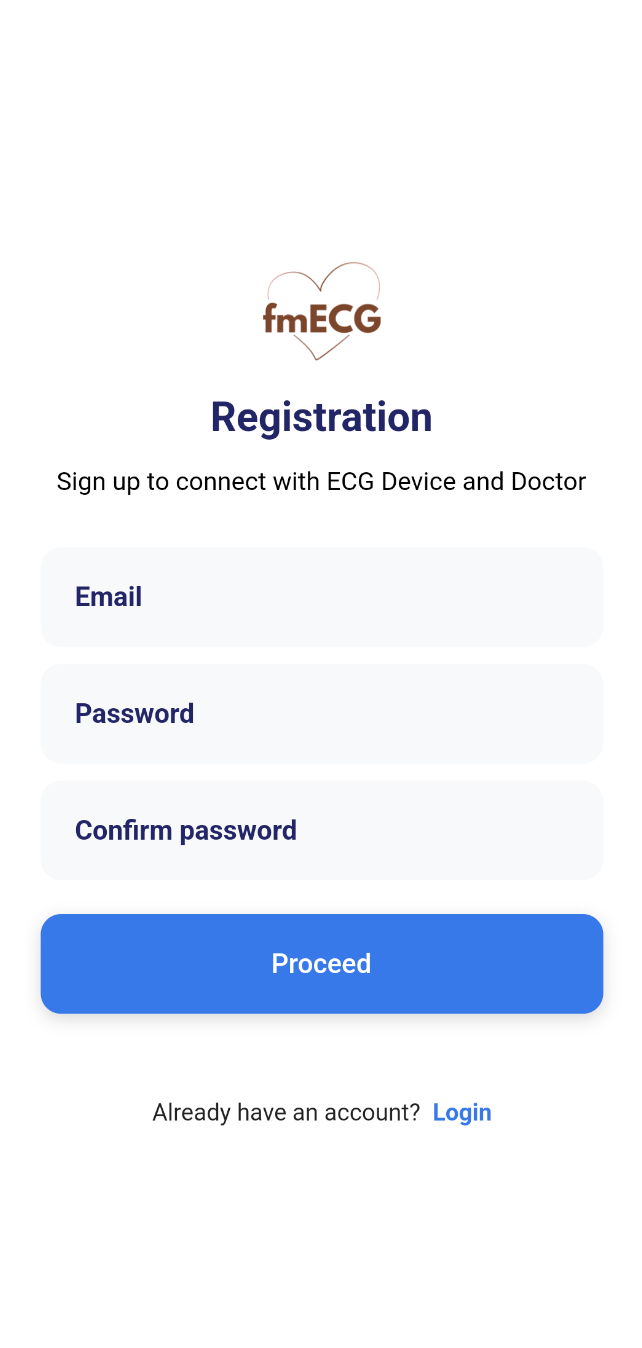
\includegraphics[width=6cm,height=12cm]{Images/mobile_app/demo/register.png}
  \caption[Giao diện trang đăng ký tài khoản]{\bfseries \fontsize{12pt}{0pt}\selectfont Giao diện trang đăng ký tài khoản}
  \label{demo_register} %đặt tên cho ảnh
\end{figure}

Trang đăng ký gồm có 3 ô để người dùng đăng ký tài khoản một cách nhanh chóng

\begin{figure}[H]
  \centering
  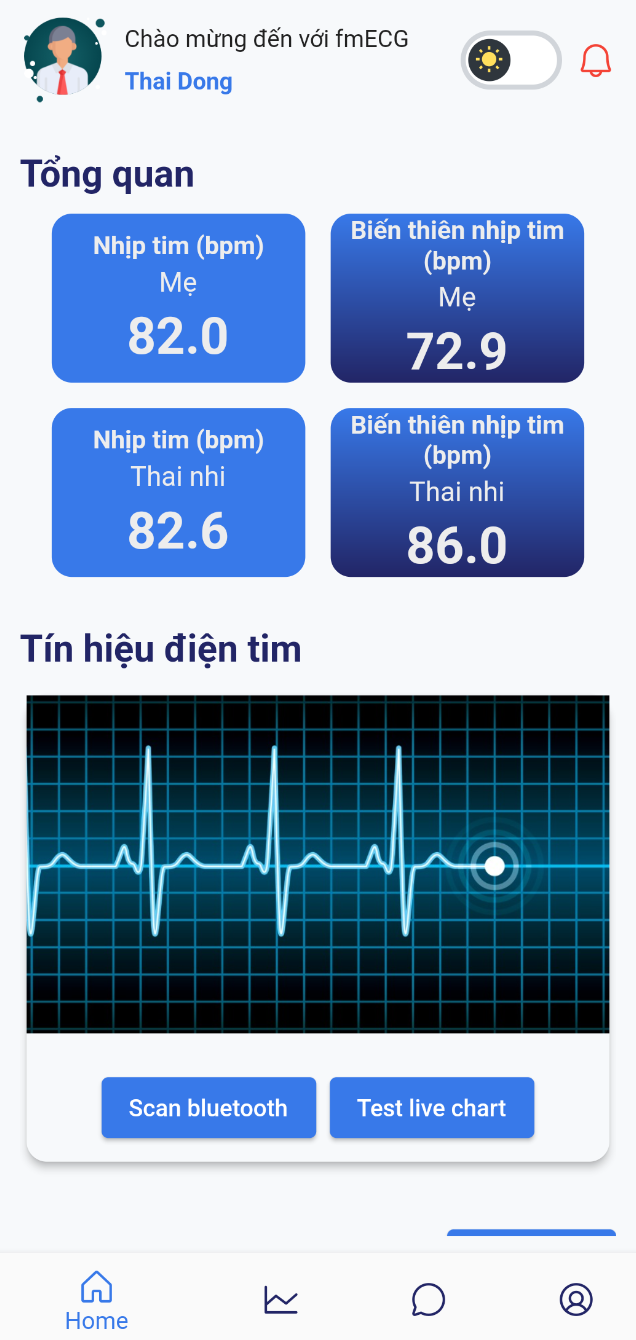
\includegraphics[width=6cm,height=12cm]{Images/mobile_app/demo/home_screen.png}
  \caption[Giao diện trang]{\bfseries \fontsize{12pt}{0pt}\selectfont Giao diện trang}
  \label{demo_} %đặt tên cho ảnh
\end{figure}

\begin{figure}[H]
  \centering
  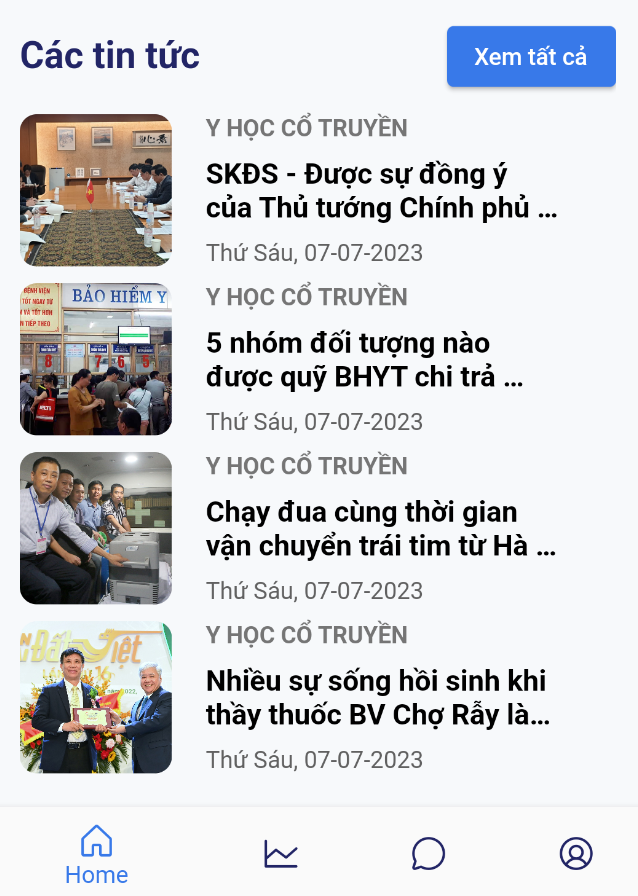
\includegraphics[width=6cm,height=8cm]{Images/mobile_app/demo/preview_news.png}
  \caption[Giao diện trang]{\bfseries \fontsize{12pt}{0pt}\selectfont Giao diện trang}
  \label{demo_} %đặt tên cho ảnh
\end{figure}

\begin{figure}[H]
  \centering
  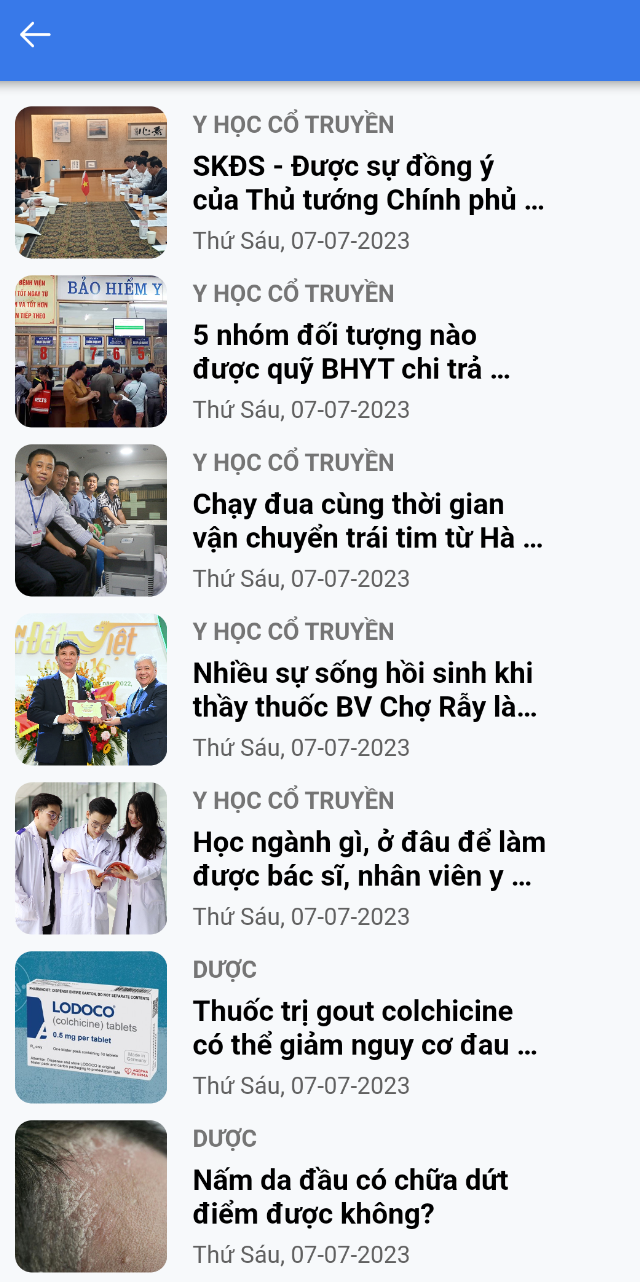
\includegraphics[width=6cm,height=12cm]{Images/mobile_app/demo/all_news.png}
  \caption[Giao diện trang]{\bfseries \fontsize{12pt}{0pt}\selectfont Giao diện trang}
  \label{demo_} %đặt tên cho ảnh
\end{figure}

\begin{figure}[H]
  \centering
  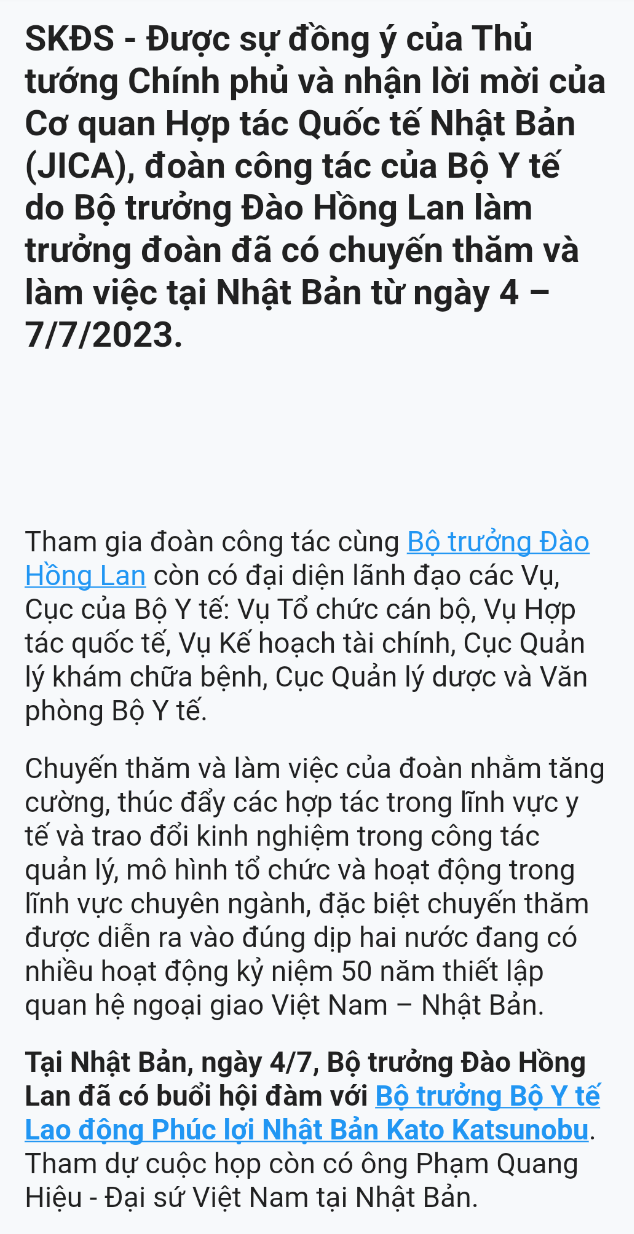
\includegraphics[width=6cm,height=12cm]{Images/mobile_app/demo/detail_news.png}
  \caption[Giao diện trang]{\bfseries \fontsize{12pt}{0pt}\selectfont Giao diện trang}
  \label{demo_} %đặt tên cho ảnh
\end{figure}

\begin{figure}[H]
  \centering
  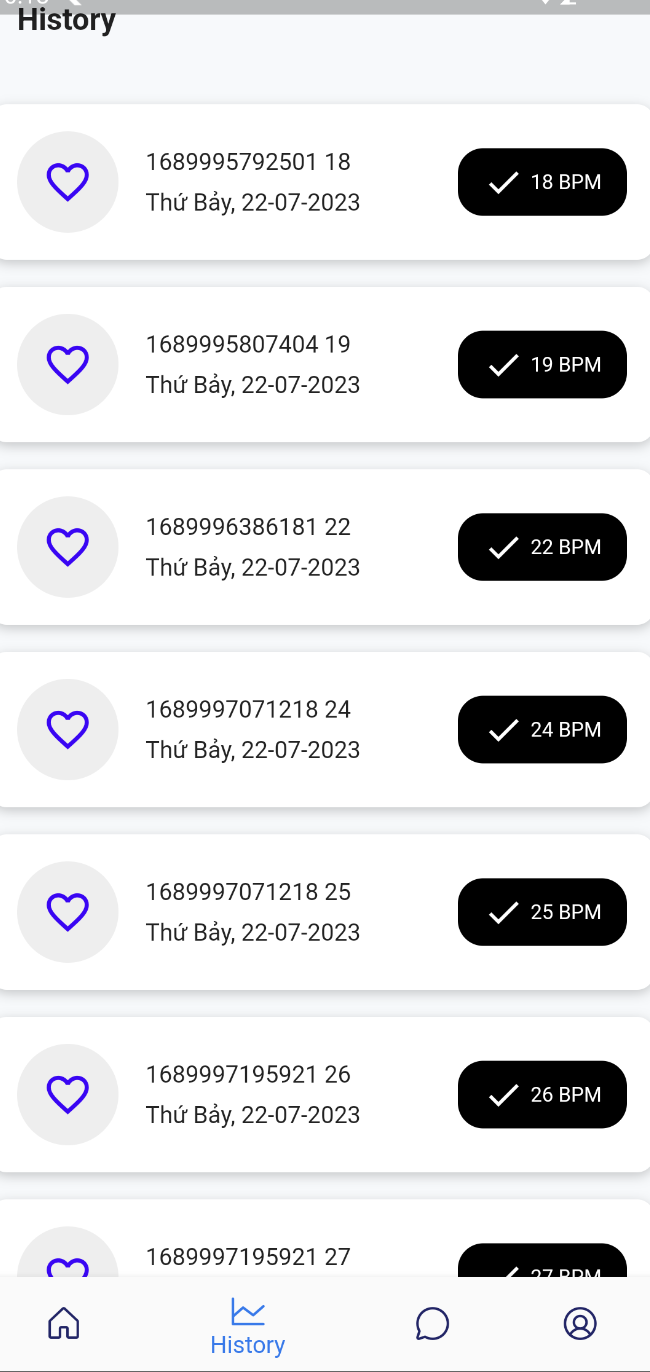
\includegraphics[width=6cm,height=12cm]{Images/mobile_app/demo/history.png}
  \caption[Giao diện trang]{\bfseries \fontsize{12pt}{0pt}\selectfont Giao diện trang}
  \label{demo_} %đặt tên cho ảnh
\end{figure}

\begin{figure}[H]
  \centering
  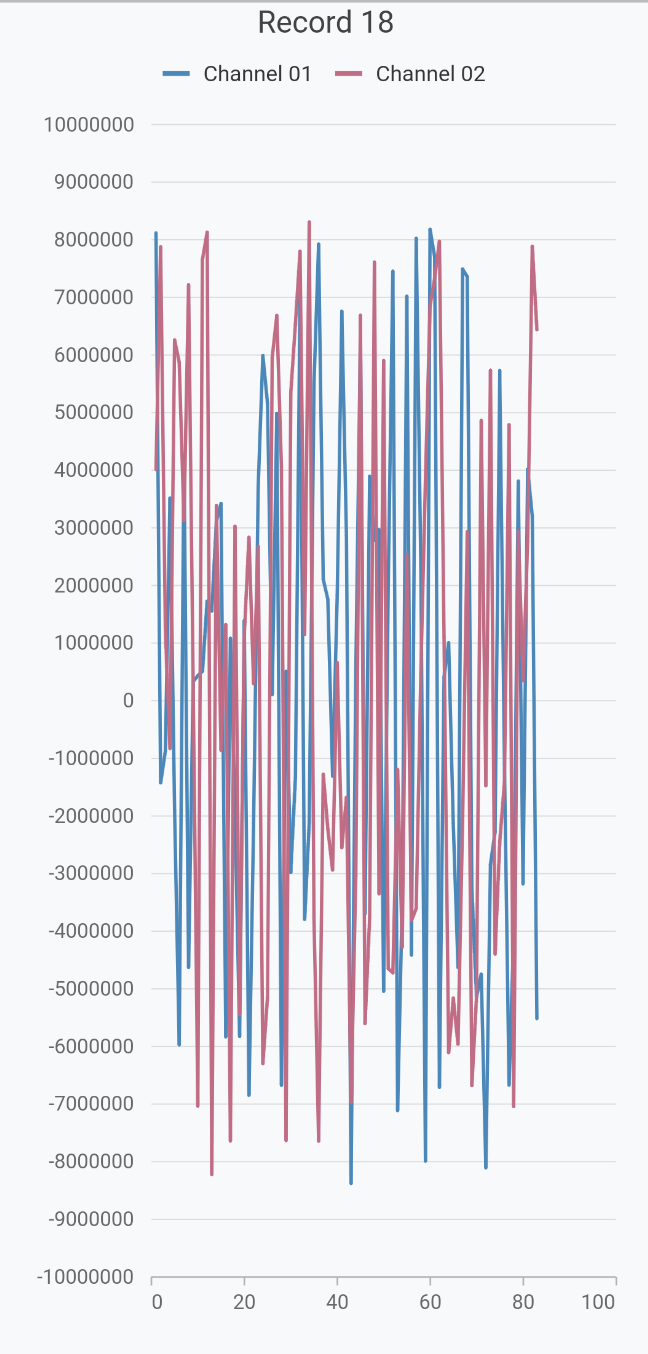
\includegraphics[width=6cm,height=12cm]{Images/mobile_app/demo/detail_record.png}
  \caption[Giao diện trang]{\bfseries \fontsize{12pt}{0pt}\selectfont Giao diện trang}
  \label{demo_} %đặt tên cho ảnh
\end{figure}

\begin{figure}[H]
  \centering
  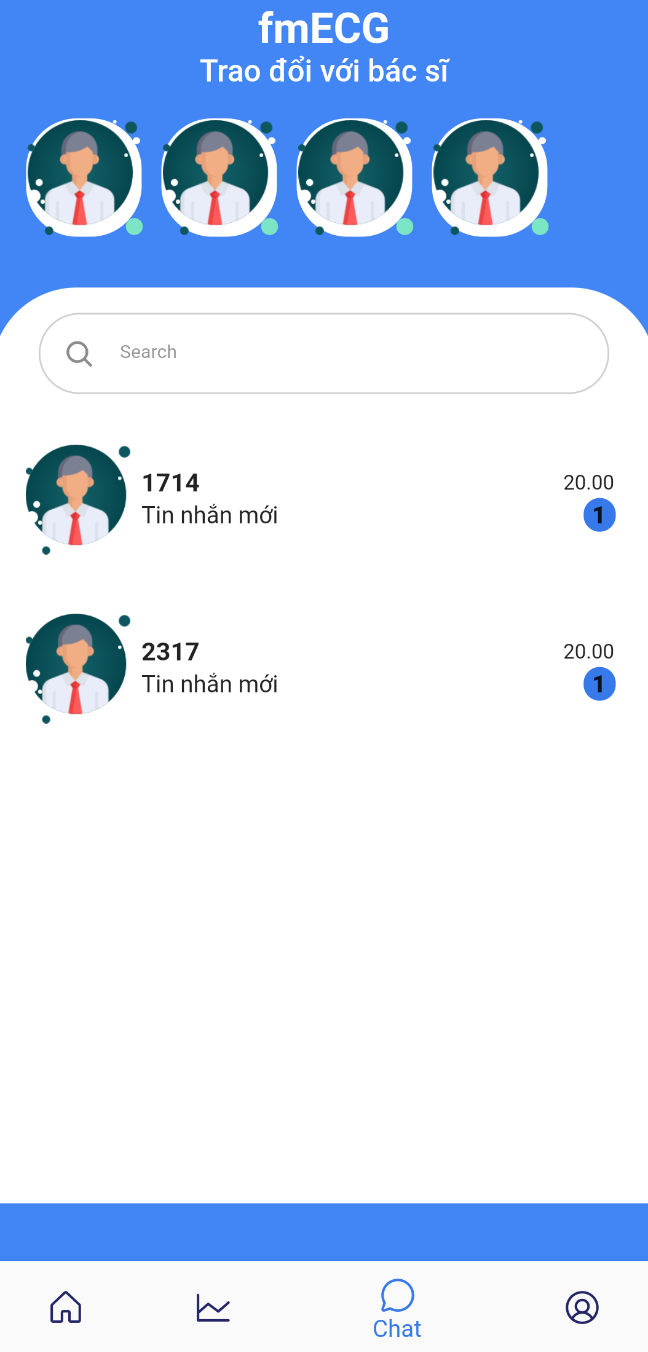
\includegraphics[width=6cm,height=12cm]{Images/mobile_app/demo/chat_preview.png}
  \caption[Giao diện trang]{\bfseries \fontsize{12pt}{0pt}\selectfont Giao diện trang}
  \label{demo_} %đặt tên cho ảnh
\end{figure}

\begin{figure}[H]
  \centering
  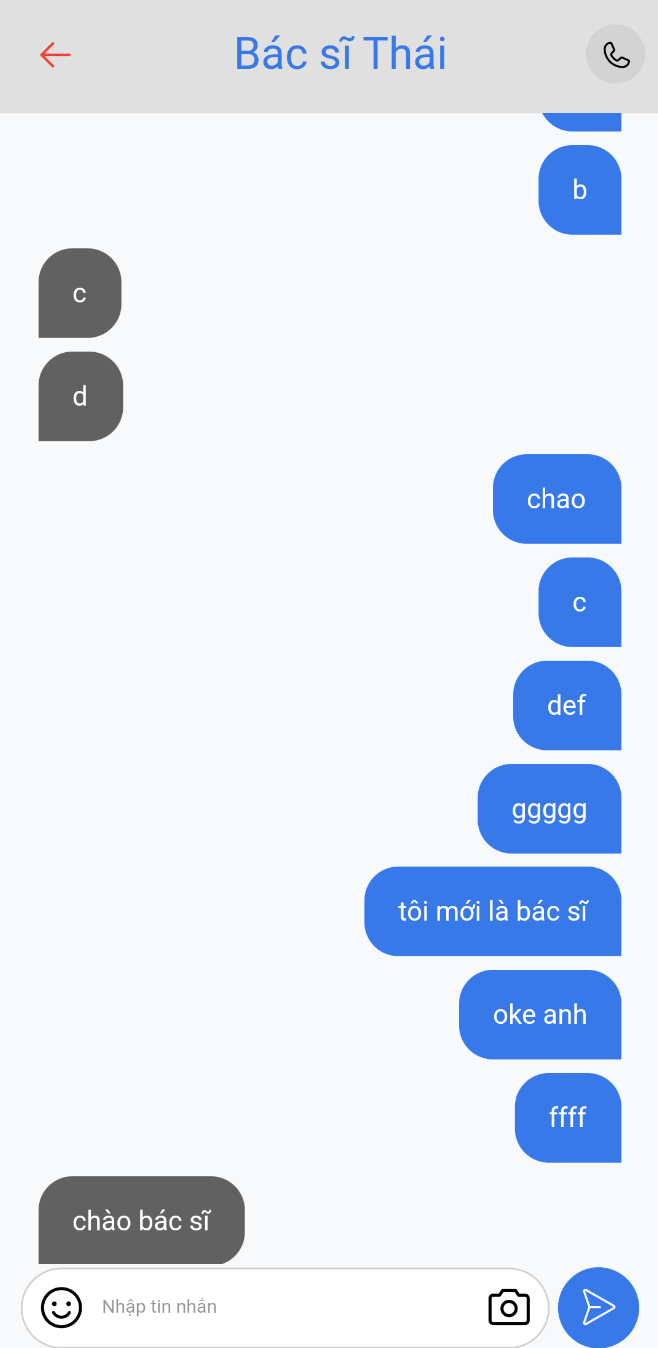
\includegraphics[width=6cm,height=12cm]{Images/mobile_app/demo/chat_detail.png}
  \caption[Giao diện trang]{\bfseries \fontsize{12pt}{0pt}\selectfont Giao diện trang}
  \label{demo_} %đặt tên cho ảnh
\end{figure}

\begin{figure}[H]
  \centering
  
\includegraphics[width=6cm,height=12cm]{Images/mobile_app/demo/off_bluetooth.png}
  \caption[Giao diện trang]{\bfseries \fontsize{12pt}{0pt}\selectfont Giao diện trang}
  \label{demo_} %đặt tên cho ảnh
\end{figure}

\begin{figure}[H]
  \centering
  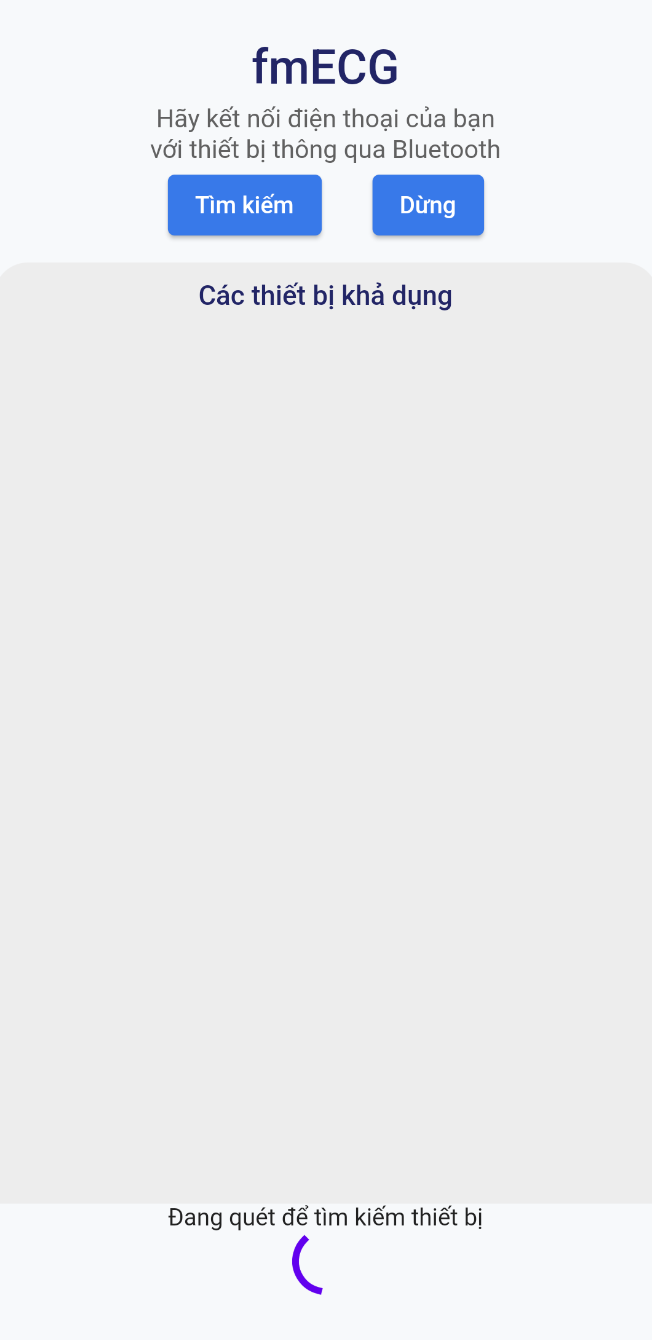
\includegraphics[width=6cm,height=12cm]{Images/mobile_app/demo/finding_bluetooth.png}
  \caption[Giao diện trang]{\bfseries \fontsize{12pt}{0pt}\selectfont Giao diện trang}
  \label{demo_} %đặt tên cho ảnh
\end{figure}



\paragraph{Website}
\mbox{}

\subsubsection{Thiết kế API}

\paragraph{API liên quan đến thông tin người dùng}
\mbox{}

\begin{table}[H]
     \centering
     \caption{\bfseries \fontsize{12pt}{0pt}\selectfont Bảng API liên quan đến thông tin người dùng}
     \begin{tabularx}{0.9\textwidth}{
     | >{\raggedright\arraybackslash}X
     | >{\raggedright\arraybackslash}m{2cm}
     | >{\raggedright\arraybackslash}X|
     }
     \hline
     \bfseries Đường dẫn    &\bfseries Phương thức    &\bfseries Mô tả\\ \hline
    api/users/profile   &   GET  &  Lấy thông tin của người dùng với đầu vào là JWT token khi người dùng đăng nhập thành công vào hệ thống \\  \hline
    api/users/profile   &    PUT    &  Cập nhật thông tin người dùng \\  \hline
    api/users/change-password   &   PUT     & Thay đổi mật khẩu của người dùng  \\ \hline
    api/users/\{:userId\}  &   GET     & Lấy thông tin của người dùng cụ thể theo user id \\ \hline

     \end{tabularx}
     \label{table_api_user}
\end{table}



\paragraph{API liên quan đến việc xác thực người dùng }
\mbox{}

\begin{table}[H]
  \centering
  \caption{\bfseries \fontsize{12pt}{0pt}\selectfont Bảng API liên quan đến việc xác thực người dùng}
  \begin{tabularx}{0.9\textwidth}{
  | >{\raggedright\arraybackslash}X
  | >{\raggedright\arraybackslash}m{2cm}
  | >{\raggedright\arraybackslash}X|
  }
  \hline
  \bfseries Đường dẫn    &\bfseries Phương thức    &\bfseries Mô tả\\ \hline
 api/register   &   POST  & Đăng ký tài khoản \\ \hline
 api/login   &    POST    & Đăng nhập vào hệ thống \\ \hline
 api/logout  &   GET     & Đăng xuất khỏi hệ thống \\ \hline
 api/reset-password  &     POST   &  Gửi reset token đến email của người dùng để reset mật khẩu \\  \hline
 api/reset-password/reset &   POST     & Giúp reset lại mật khẩu mới với verify token được nhận từ api: api/reset-password  \\ \hline

  \end{tabularx}
  \label{table_api_auth}
\end{table}



\paragraph{API liên quan đến tin tức}
\mbox{}

\begin{table}[H]
  \centering
  \caption{\bfseries \fontsize{12pt}{0pt}\selectfont Bảng API liên quan đến tin tức}
  \begin{tabularx}{0.9\textwidth}{
  | >{\raggedright\arraybackslash}X
  | >{\raggedright\arraybackslash}m{2cm}
  | >{\raggedright\arraybackslash}X|
  }
  \hline
  \bfseries Đường dẫn    &\bfseries Phương thức    &\bfseries Mô tả\\ \hline
 api/news/\{:newsId\}   &   GET  & Lấy nội của tin tức tương ứng với id dưới dạng HTML \\ \hline
 api/news   &    GET    & Lấy toàn bộ danh sách thông tin của tin tức \\ \hline
 api/categories  &   GET     & Lấy toàn bộ danh sách thông tin của tin tức \\ \hline
 api/category/\{:categoryId\}   &     GET   & Lấy thông tin của loại tin tức theo id tương ứng \\ \hline
 api/ news/category/\{:categoryId\} &   GET     & Lấy toàn bộ thông tin của tin tức theo id của loại tin \\ \hline

  \end{tabularx}
  \label{table_api_news}
\end{table}

\paragraph{API liên quan đến bản ghi ECG}
\mbox{}

\begin{table}[H]
  \centering
  \caption{\bfseries \fontsize{12pt}{0pt}\selectfont Bảng API liên quan đến bản ghi ECG}
  \begin{tabularx}{0.9\textwidth}{
  | >{\raggedright\arraybackslash}X
  | >{\raggedright\arraybackslash}m{2cm}
  | >{\raggedright\arraybackslash}X|
  }
  \hline
  \bfseries Đường dẫn    &\bfseries Phương thức    &\bfseries Mô tả\\ \hline
 api/ecg-records/upload   &   POST  & Tải dữ liệu của phiên đo ECG lên server \\ \hline
 api/ecg-records/patient/\{:patientId\}   &    GET    & Lấy danh sách thông tin các phiên đo ECG của bệnh nhân \\ \hline
 api/ecg-records/doctor/\{:doctorId\} &   GET     & Lấy danh sách thông tin các phiên đo ECG của các bệnh nhân được quản lý bởi bác sỹ \\ \hline
 api/ecg-records/record-data/\{:recordId\}  &     GET   & Lấy dữ liệu một phiên đo của bệnh nhân \\ \hline

  \end{tabularx}
  \label{table_api_ecg}
\end{table}



\paragraph{API liên quan liên quan đến việc phân công bệnh nhân cho bác sỹ}
\mbox{}

\begin{table}[H]
  \centering
  \caption{\bfseries \fontsize{12pt}{0pt}\selectfont Bảng API liên quan liên quan đến việc phân công bệnh nhân cho bác sỹ}
  \begin{tabularx}{0.9\textwidth}{
  | >{\raggedright\arraybackslash}X
  | >{\raggedright\arraybackslash}m{2cm}
  | >{\raggedright\arraybackslash}X|
  }
  \hline
  \bfseries Đường dẫn    &\bfseries Phương thức    &\bfseries Mô tả\\ \hline
   api/doctor/\{:doctorId\}/patients   &   GET  & Lấy danh sách thông tin bệnh nhân được phân công cho bác sĩ \\ \hline
  api/patient/\{:patientId\}/doctor  &    GET    & Lấy thông tin bác sỹ được phân công cho bệnh nhân \\ \hline

  \end{tabularx}
  \label{table_api_pat_doc}
\end{table}






\subsubsection{Sơ đồ lớp}

\paragraph{Ứng dụng}
\mbox{}

\paragraph{Server và Website quản trị hệ thống}
\mbox{}

\begin{enumerate}[a)]
\item Danh sách các class diagram

\begin{figure}[H]
  \centering
  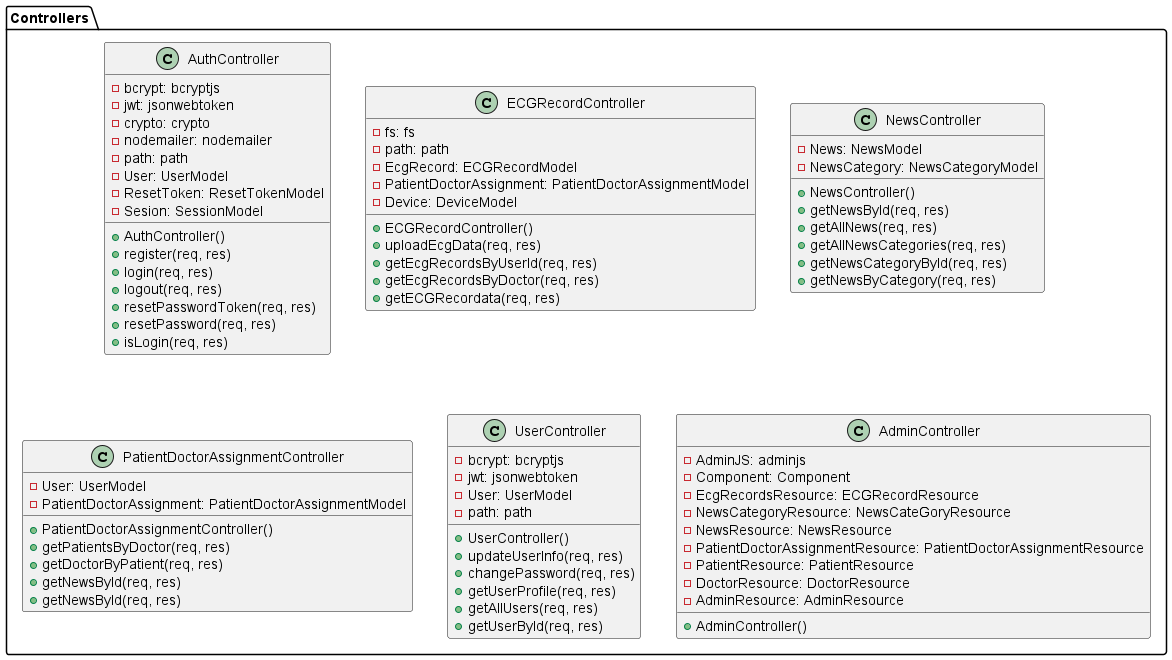
\includegraphics[width=16cm,height=13cm]{Images/server/class/class_controller.png}
  \caption[Sơ đồ lớp của package Controllers]{\bfseries \fontsize{12pt}{0pt}\selectfont Sơ đồ lớp của package Controllers}
  \label{class_controller} %đặt tên cho ảnh
\end{figure}



\begin{figure}[H]
  \centering
  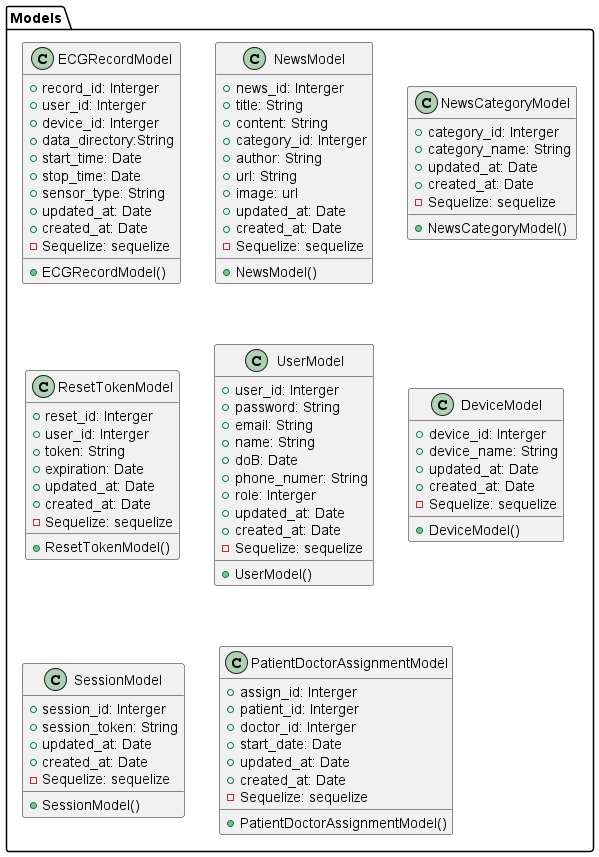
\includegraphics[width=15cm,height=16cm]{Images/server/class/class_model.png}
  \caption[Sơ đồ lớp của package Models]{\bfseries \fontsize{12pt}{0pt}\selectfont Sơ đồ lớp của package Models}
  \label{class_model} %đặt tên cho ảnh
\end{figure}


\begin{figure}[H]
  \centering
  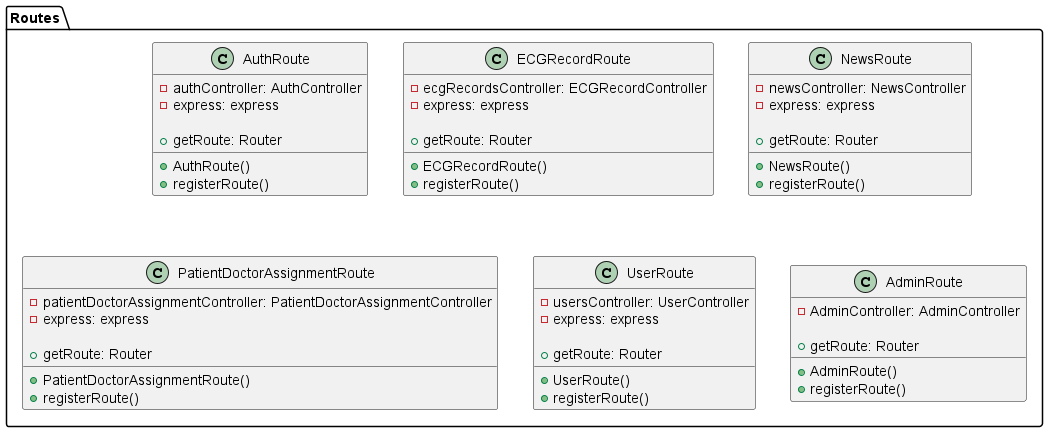
\includegraphics[width=14cm,height=6cm]{Images/server/class/class_route.png}
  \caption[Sơ đồ lớp của package Routes]{\bfseries \fontsize{12pt}{0pt}\selectfont Sơ đồ lớp của package Routes}
  \label{class_route} %đặt tên cho ảnh
\end{figure}


\begin{figure}[H]
  \centering
  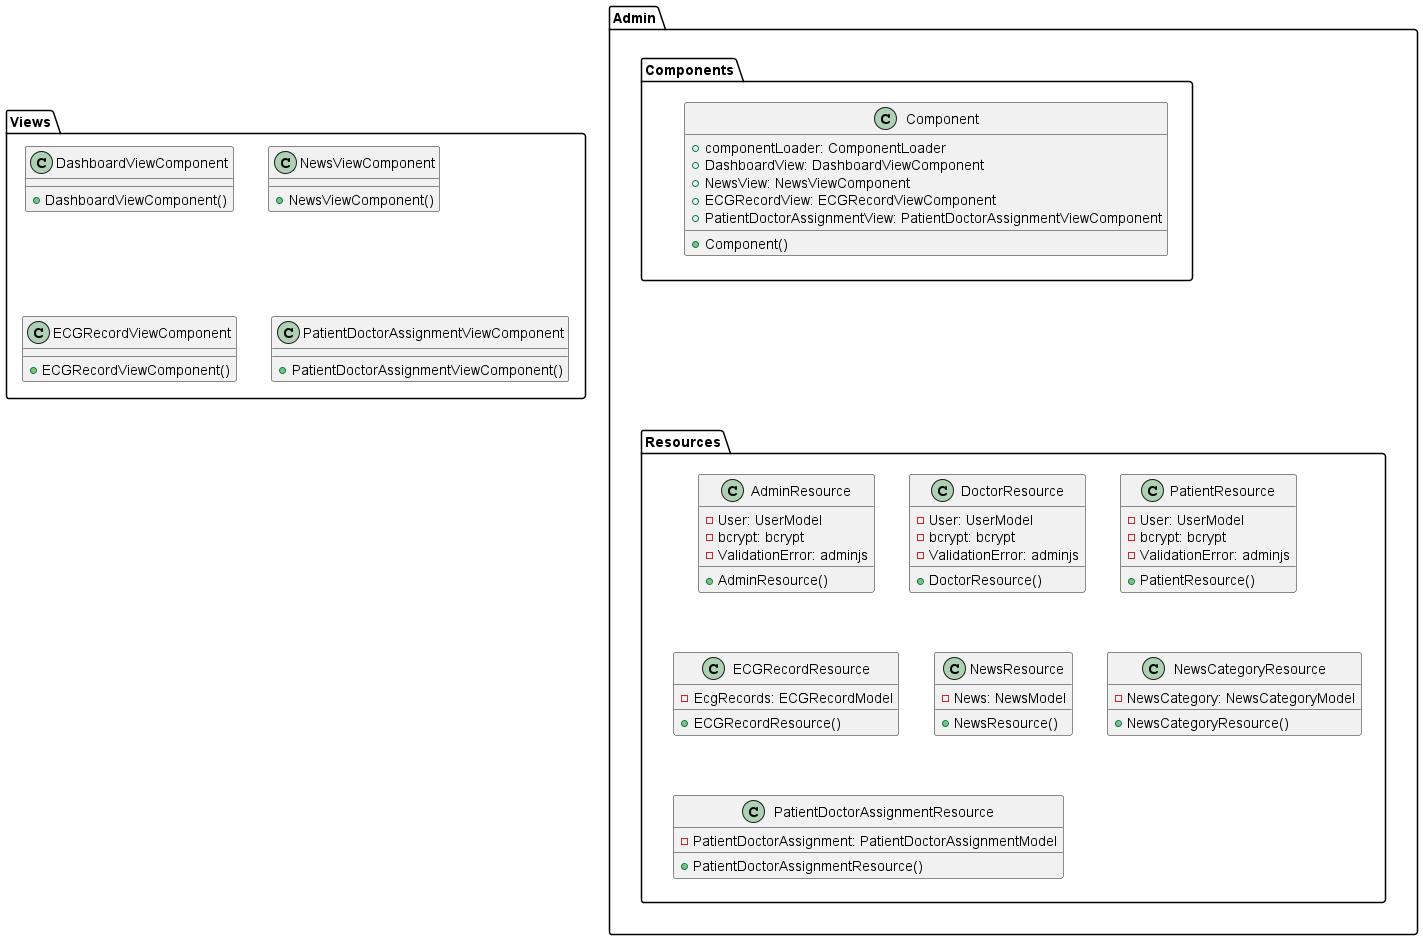
\includegraphics[width=15cm,height=14cm]{Images/server/class/class_admin.png}
  \caption[Sơ đồ lớp của package View và Admin]{\bfseries \fontsize{12pt}{0pt}\selectfont Sơ đồ lớp của package View và Admin}
  \label{class_admin} %đặt tên cho ảnh
\end{figure}


\begin{itemize}

  \item Package "Controllers":

  Chứa các controllers xử lý logic và điều khiển các yêu cầu từ người dùng.
  \item Package "Models":
  
  Chứa các lớp đại diện cho các đối tượng của cơ sở dữ liệu, định nghĩa các thuộc tính và phương thức để làm việc với dữ liệu.
  \item Package "Routes":
  
  Chứa các lớp route, xác định các endpoint và xử lý các yêu cầu HTTP từ người dùng bằng cách gọi tới các controllers tương ứng.
  \item Package "Views":
  
  Chứa các view components đại diện cho giao diện người dùng.
  \item Package "Admin":
  
  Chứa các thành phần liên quan đến trang Admin dashboard.
  \item Package "Resources" (Trong "Admin"):
  
  Chứa các lớp Resource (nguồn tài nguyên) đại diện cho các tài nguyên của trang Admin dashboard, bao gồm: AdminResource, DoctorResource, PatientResource, ECGRecordResource, NewsResource, NewsCategoryResource và PatientDoctorAssignmentResource.
  \item Package "Components" (Trong "Admin"):
  
  Chứa các lớp Components đại diện cho các thành phần giao diện của trang Admin dashboard, bao gồm: ComponentLoader, DashboardViewComponent, NewsViewComponent, ECGRecordViewComponent và PatientDoctorAssignmentViewComponent.
\end{itemize}



\item Mối quan hệ

\begin{figure}[H]
  \centering
  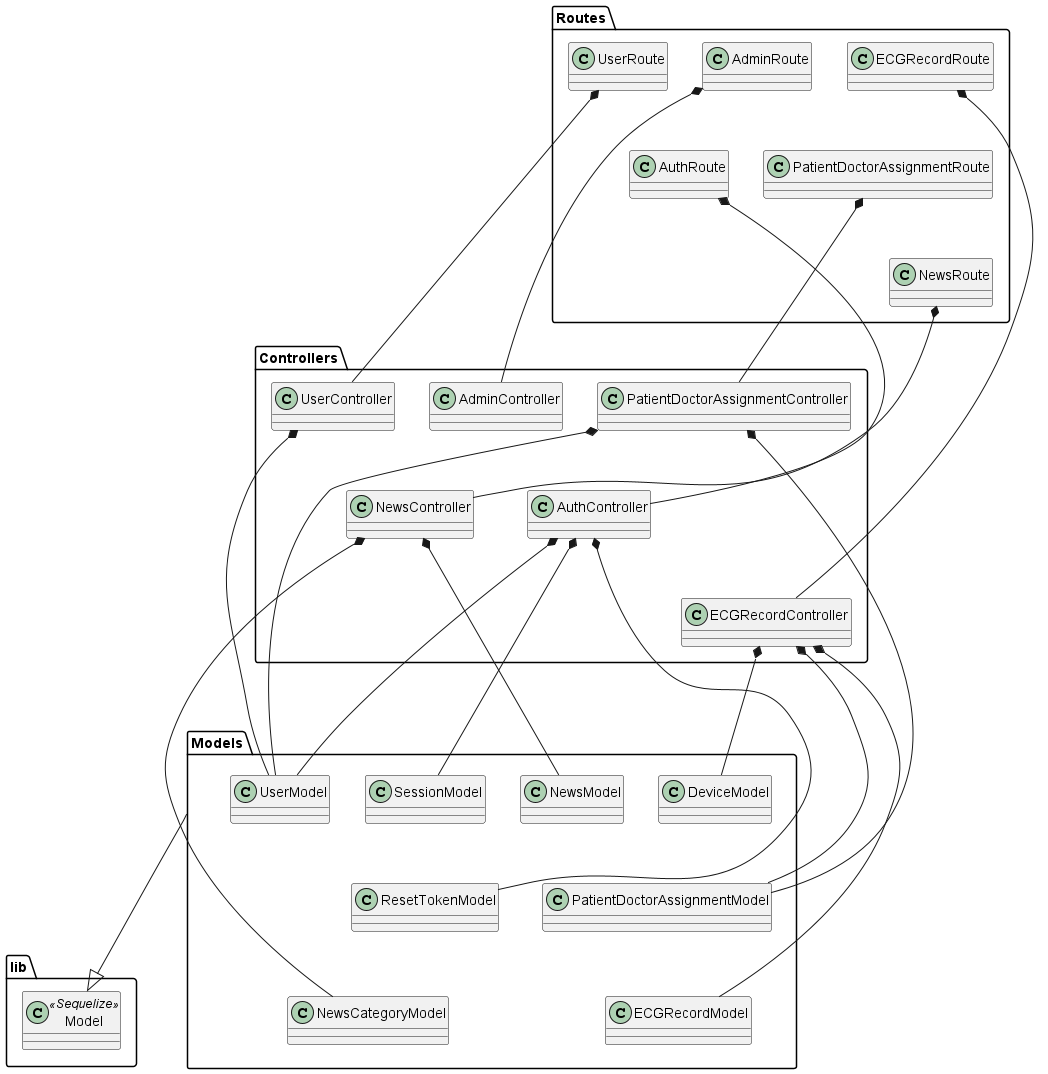
\includegraphics[width=15cm,height=12cm]{Images/server/class/class_relation.png}
  \caption[Mối quan hệ giữa các class ở phía server]{\bfseries \fontsize{12pt}{0pt}\selectfont Mối quan hệ giữa các class ở phía server}
  \label{class_relation} %đặt tên cho ảnh
\end{figure}


\begin{figure}[H]
  \centering
  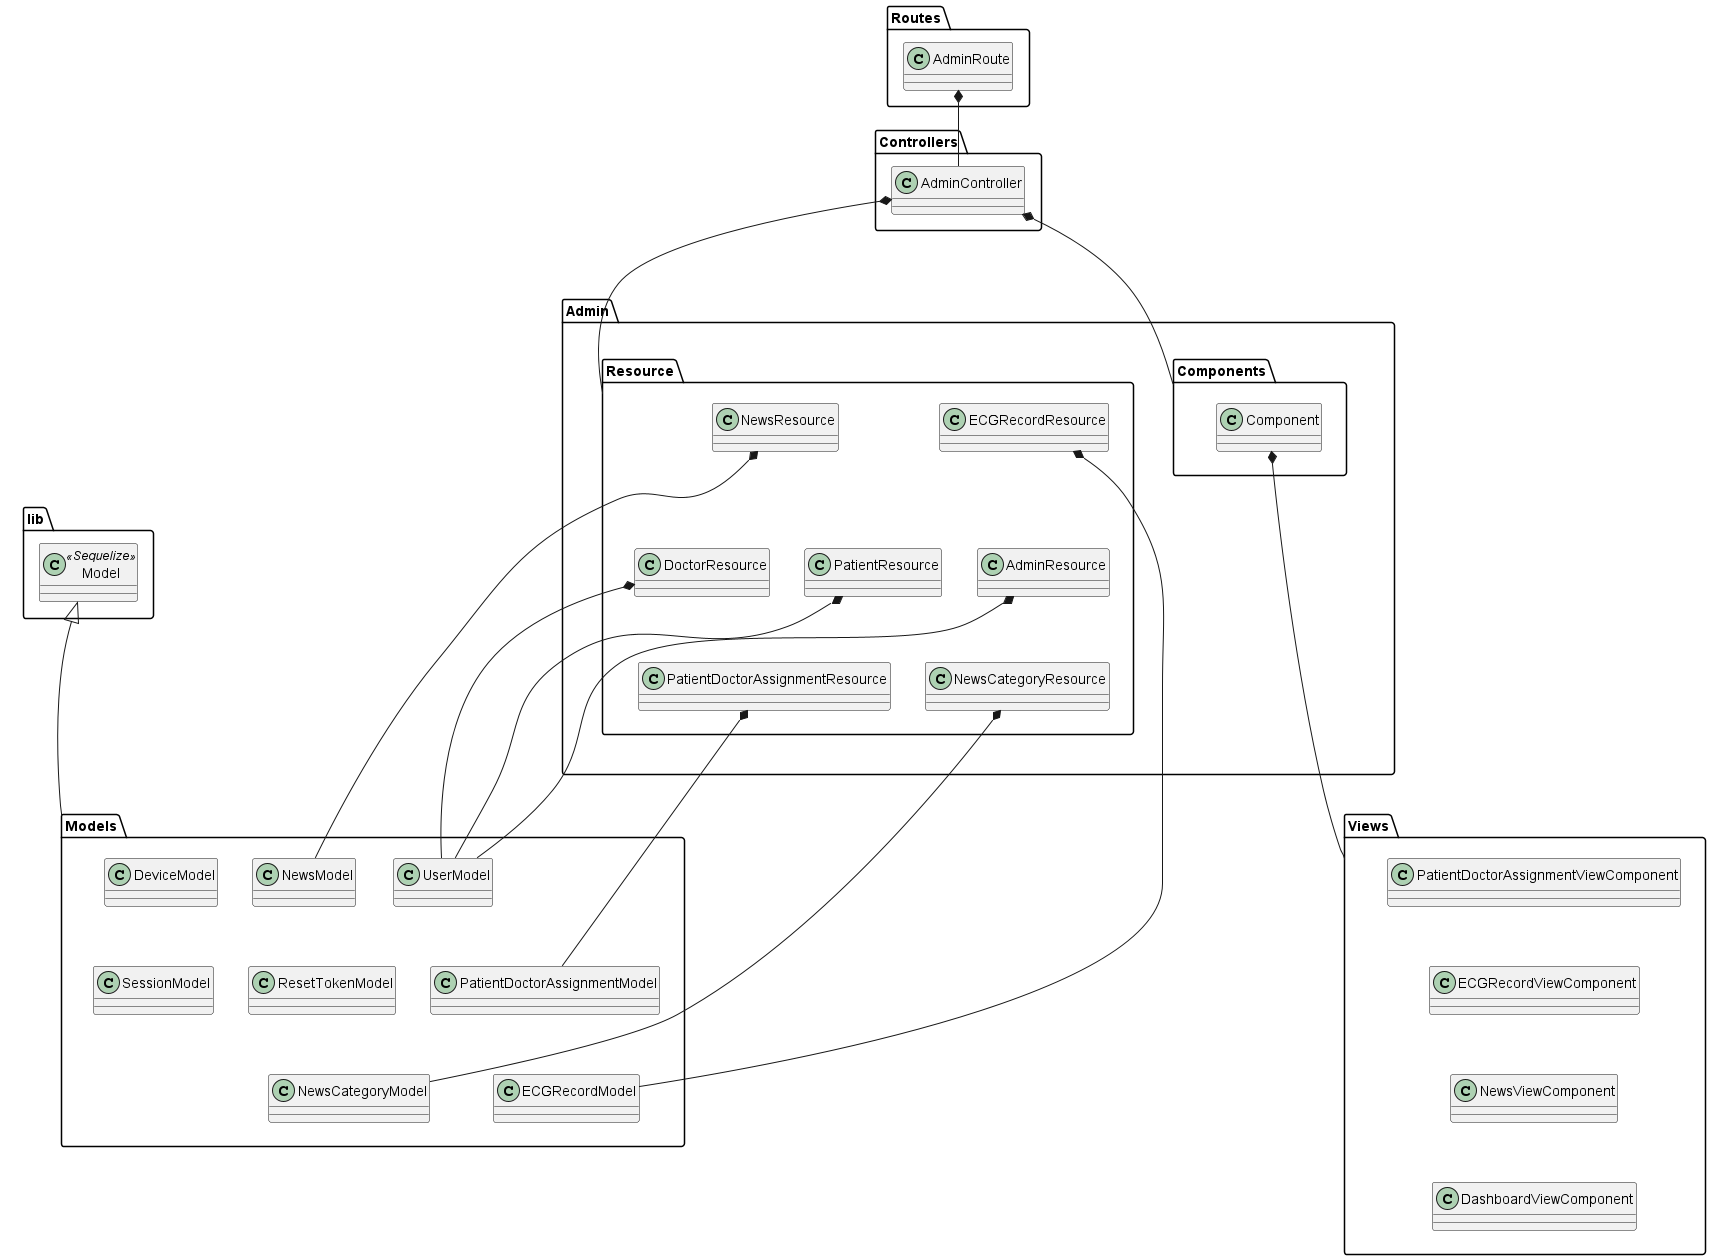
\includegraphics[width=16cm,height=15cm]{Images/server/class/class_admin_relation.png}
  \caption[Mối quan hệ giữa các class ở phía website quản trị]{\bfseries \fontsize{12pt}{0pt}\selectfont Mối quan hệ giữa các class ở phía website quản trị}
  \label{class_admin_relation} %đặt tên cho ảnh
\end{figure}

\end{enumerate}




\subsubsection{Sơ đồ tuần tự}

% ------------------------User----------------------

\paragraph{API liên quan đến thông tin người dùng}
\mbox{}


% sửa lại ảnh 
\begin{figure}[H]
  \centering
  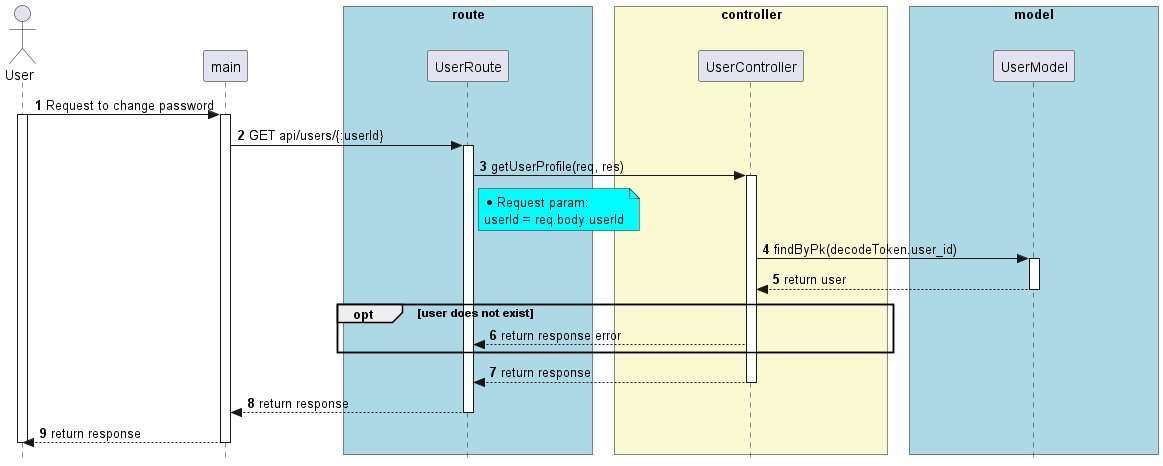
\includegraphics[width=16cm,height=9cm]{Images/server/sequence/server/getUserById.png}
  \caption[Sơ đồ tuần tự cho API lấy thông tin của người dùng dựa trên ID ]{\bfseries \fontsize{12pt}{0pt}
  \selectfont Sơ đồ tuần tự cho API lấy thông tin của người dùng dựa trên ID }
  \label{getUserById} %đặt tên cho ảnh
\end{figure}
Hình \ref{getUserById} mô tả quá trình lấy thông tin người dùng dựa trên ID trong ứng dụng. Người dùng gửi yêu cầu lấy thông tin người dùng theo ID, thông qua các tầng của hệ thống, yêu cầu này được xử lý bởi UserController. UserController kiểm tra thông tin và truy vấn UserModel để lấy thông tin người dùng. Nếu người dùng không tồn tại, hệ thống trả về response lỗi, ngược lại, response chứa thông tin người dùng được gửi lại từ UserController tới người dùng.


% sửa lại ảnh 
\begin{figure}[H]
  \centering
  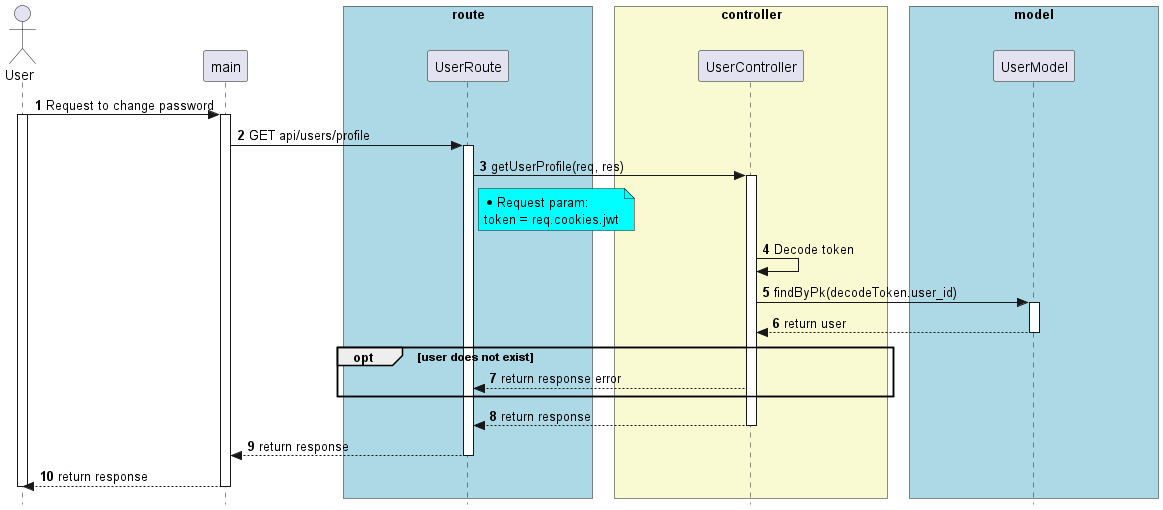
\includegraphics[width=16cm,height=9cm]{Images/server/sequence/server/getUserProfile.png}
  \caption[Sơ đồ tuần tự cho API lấy thông tin của người dùng dựa trên JWT token ]{\bfseries \fontsize{12pt}{0pt}
  \selectfont Sơ đồ tuần tự cho API lấy thông tin của người dùng dựa trên JWT token }
  \label{getUserProfile} %đặt tên cho ảnh
\end{figure}
Hình \ref{getUserProfile} mô tả quá trình lấy thông tin hồ sơ người dùng trong ứng dụng. Người dùng gửi yêu cầu lấy thông tin hồ sơ, thông qua các tầng của hệ thống, yêu cầu này được xử lý bởi UserController. UserController giải mã mã thông báo (token) để xác định người dùng, sau đó truy vấn UserModel để lấy thông tin hồ sơ của người dùng dựa trên user\_id từ mã giải mã. Nếu người dùng không tồn tại, hệ thống trả về response lỗi, ngược lại, response chứa thông tin hồ sơ của người dùng được gửi lại từ UserController tới người dùng.




% \linebreak


\begin{figure}[H]
  \centering
  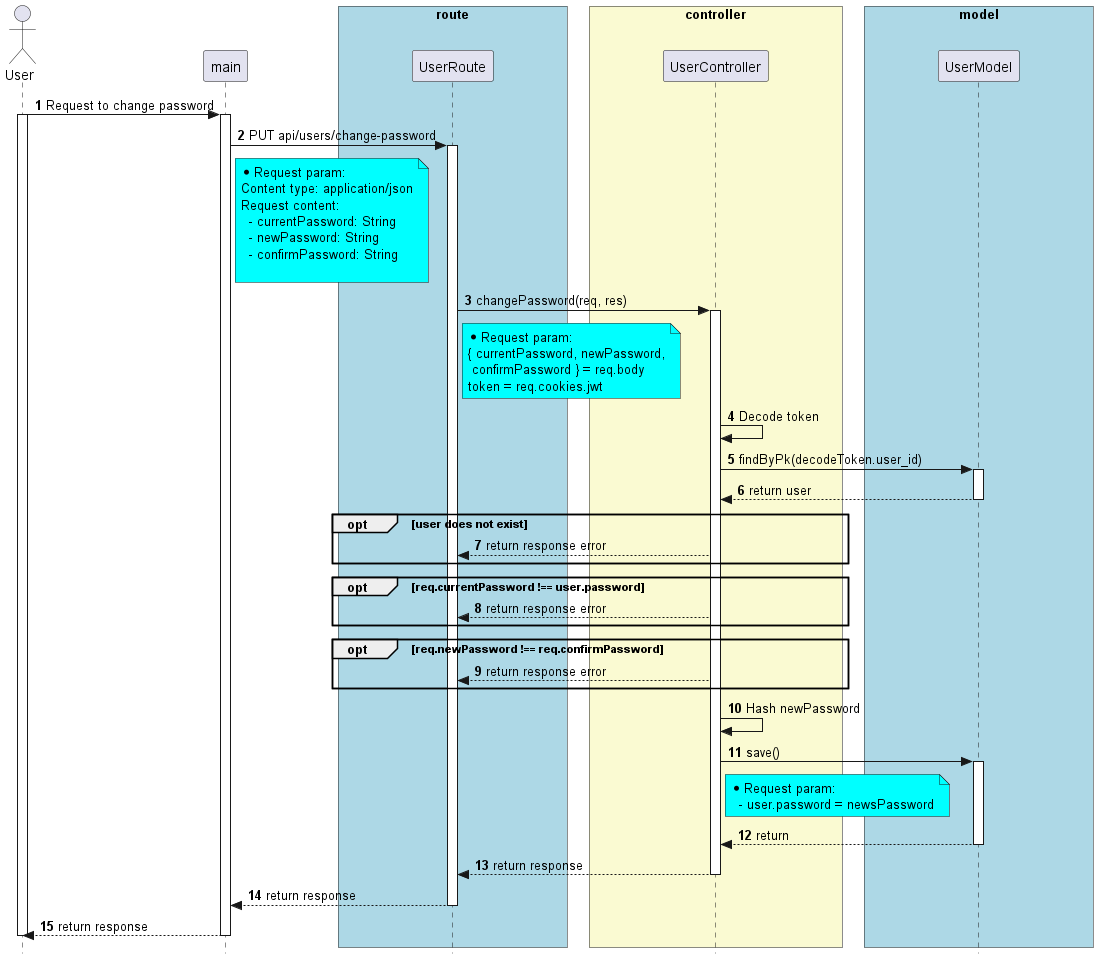
\includegraphics[width=14cm,height=15cm]{Images/server/sequence/server/changePassword.png}
  \caption[Sơ đồ tuần tự cho API thay đổi mật khẩu người dùng ]{\bfseries \fontsize{12pt}{0pt}
  \selectfont Sơ đồ tuần tự cho API thay đổi mật khẩu người dùng }
  \label{changePassword} %đặt tên cho ảnh
\end{figure}

Hình \ref{changePassword} mô tả quá trình thay đổi mật khẩu người dùng trong ứng dụng. Người dùng gửi yêu cầu thay đổi mật khẩu, thông qua các tầng của hệ thống, yêu cầu này được xử lý bởi UserController. Đầu tiên, hệ thống sẽ kiểm tra và giải mã mã thông báo (token) để xác định người dùng. Sau đó, UserController truy vấn UserModel để tìm người dùng dựa trên user\_id từ mã giải mã. Nếu người dùng không tồn tại hoặc mật khẩu hiện tại không khớp với mật khẩu trong hệ thống, hoặc mật khẩu mới không khớp với xác nhận mật khẩu, hệ thống sẽ trả về response lỗi tương ứng. Ngược lại, mật khẩu mới sẽ được mã hóa và lưu vào UserModel, sau đó hệ thống trả về response thành công tới người dùng.



\begin{figure}[H]
  \centering
  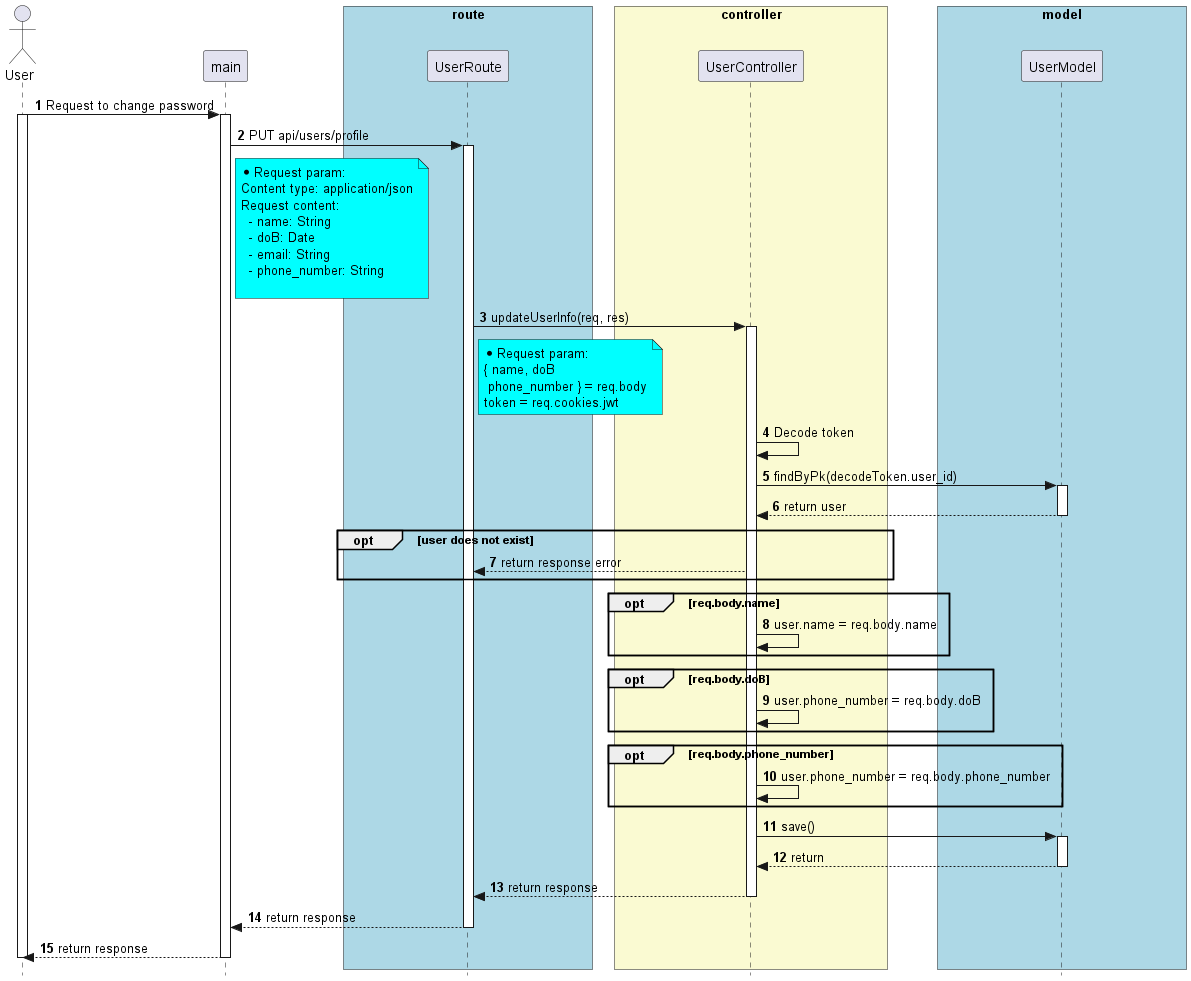
\includegraphics[width=16cm,height=12cm]{Images/server/sequence/server/updateUserInfo.png}
  \caption[Sơ đồ tuần tự cho API cập nhật thông tin người dùng ]{\bfseries \fontsize{12pt}{0pt}
  \selectfont Sơ đồ tuần tự cho API cập nhật thông tin người dùng }
  \label{updateUserInfo} %đặt tên cho ảnh
\end{figure}

Hình \ref{updateUserInfo} mô tả quá trình cập nhật thông tin người dùng trong ứng dụng. Người dùng gửi yêu cầu cập nhật thông tin, thông qua các tầng của hệ thống, yêu cầu này được xử lý bởi UserController. Đầu tiên, hệ thống sẽ kiểm tra và giải mã mã thông báo (token) để xác định người dùng. Sau đó, UserController truy vấn UserModel để tìm người dùng dựa trên user\_id từ mã giải mã. Nếu người dùng không tồn tại, hệ thống sẽ trả về response lỗi. Ngược lại, thông tin cập nhật như tên, ngày sinh (dob), và số điện thoại (phone\_number) sẽ được cập nhật vào UserModel. Sau đó, hệ thống trả về response thành công tới người dùng.


% ----------------------------------------------



% ------------------------Auth----------------------

\paragraph{API liên quan đến việc xác thực người dùng }
\mbox{}


\begin{figure}[H]
  \centering
  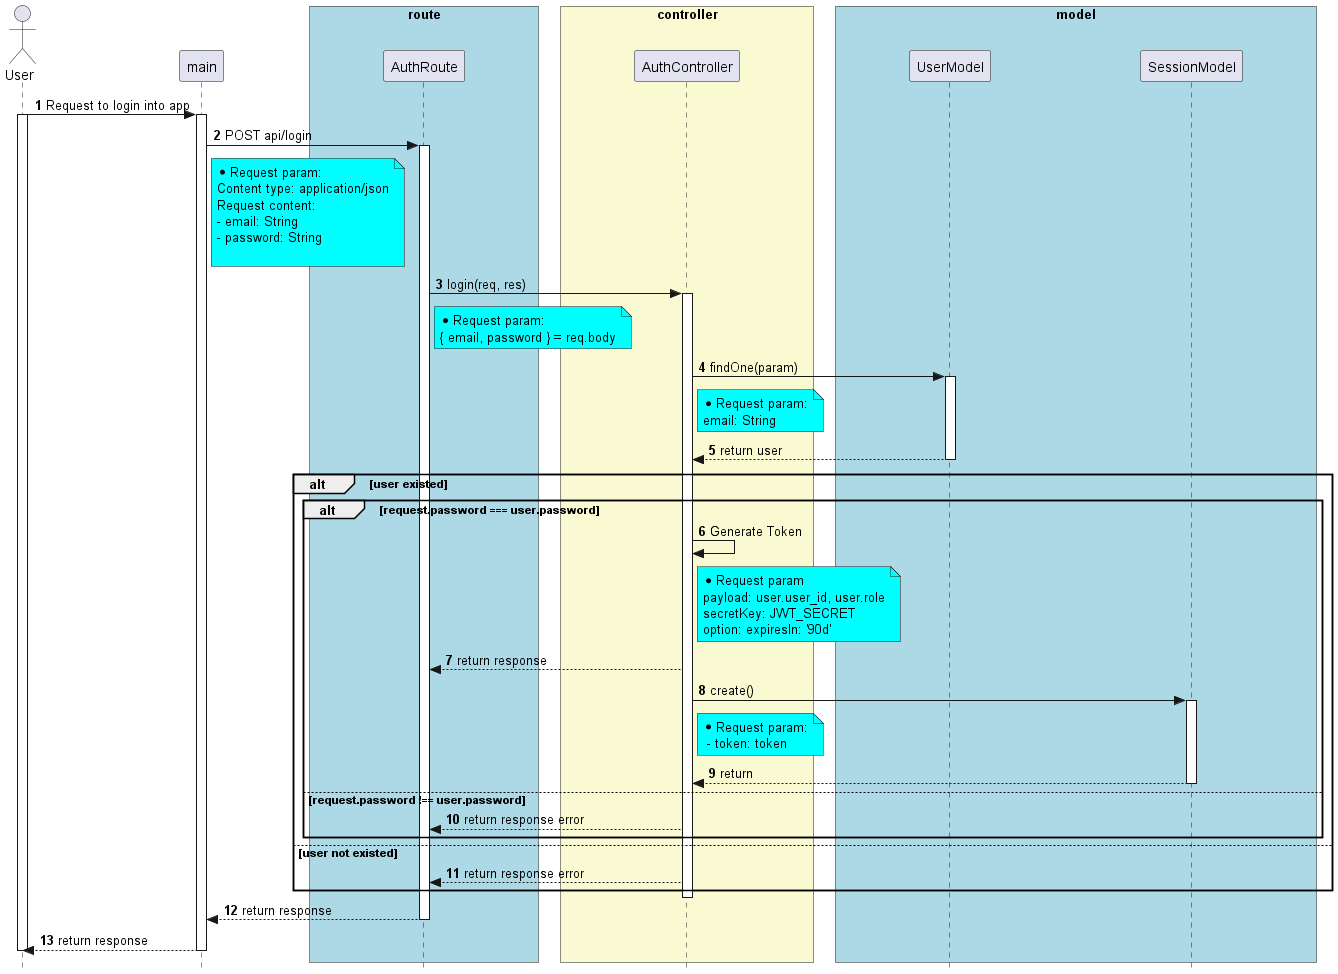
\includegraphics[width=16cm,height=12cm]{Images/server/sequence/server/login.png}
  \caption[Sơ đồ tuần tự cho API đăng nhập vào hệ thống]{\bfseries \fontsize{12pt}{0pt}
  \selectfont Sơ đồ tuần tự cho API đăng nhập vào hệ thống }
  \label{backend_login} %đặt tên cho ảnh
\end{figure}
Hình \ref{backend_login}  mô tả quá trình xác thực người dùng đăng nhập vào ứng dụng. Người dùng gửi yêu cầu đăng nhập, thông qua các tầng của hệ thống, yêu cầu này được xử lý bởi AuthController. AuthController kiểm tra thông tin người dùng, tạo token nếu đúng thông tin đăng nhập và trả về response cho người dùng.

\begin{figure}[H]
  \centering
  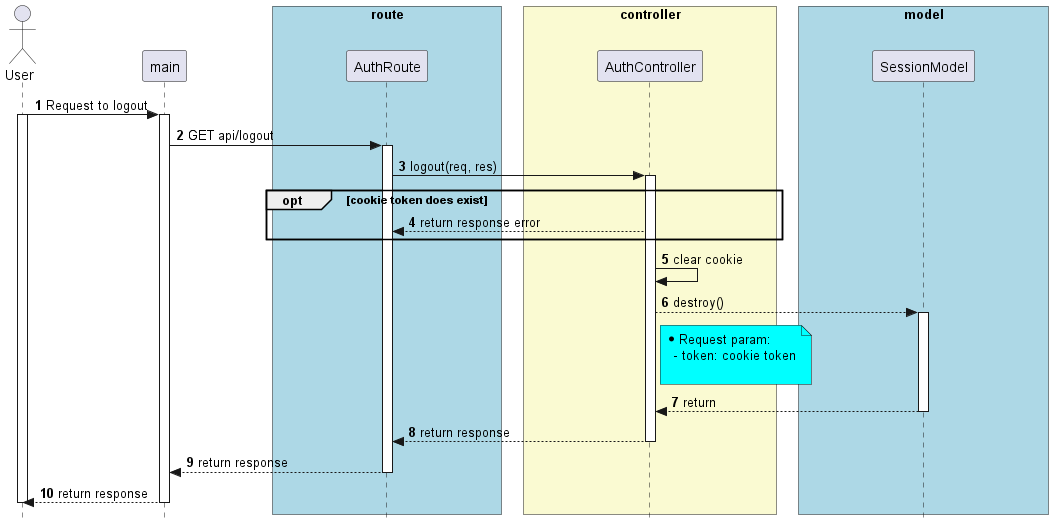
\includegraphics[width=16cm,height=9cm]{Images/server/sequence/server/logout.png}
  \caption[Sơ đồ tuần tự cho API đăng xuất khỏi hệ thống ]{\bfseries \fontsize{12pt}{0pt}
  \selectfont Sơ đồ tuần tự cho API đăng xuất khỏi hệ thống }
  \label{backend_logout} %đặt tên cho ảnh
\end{figure}
Hình \ref{backend_logout} mô tả quá trình đăng xuất (logout) người dùng khỏi ứng dụng. Người dùng gửi yêu cầu đăng xuất, thông qua các tầng của hệ thống, yêu cầu này được xử lý bởi AuthController. Đầu tiên, hệ thống kiểm tra xem cookie token có tồn tại hay không. Nếu không tồn tại, hệ thống trả về response lỗi. Ngược lại, AuthController xóa cookie và gọi tới SessionModel để hủy phiên đăng nhập của người dùng dựa trên token trong cookie. Sau khi xử lý, hệ thống trả về response thành công tới người dùng.

\begin{figure}[H]
  \centering
  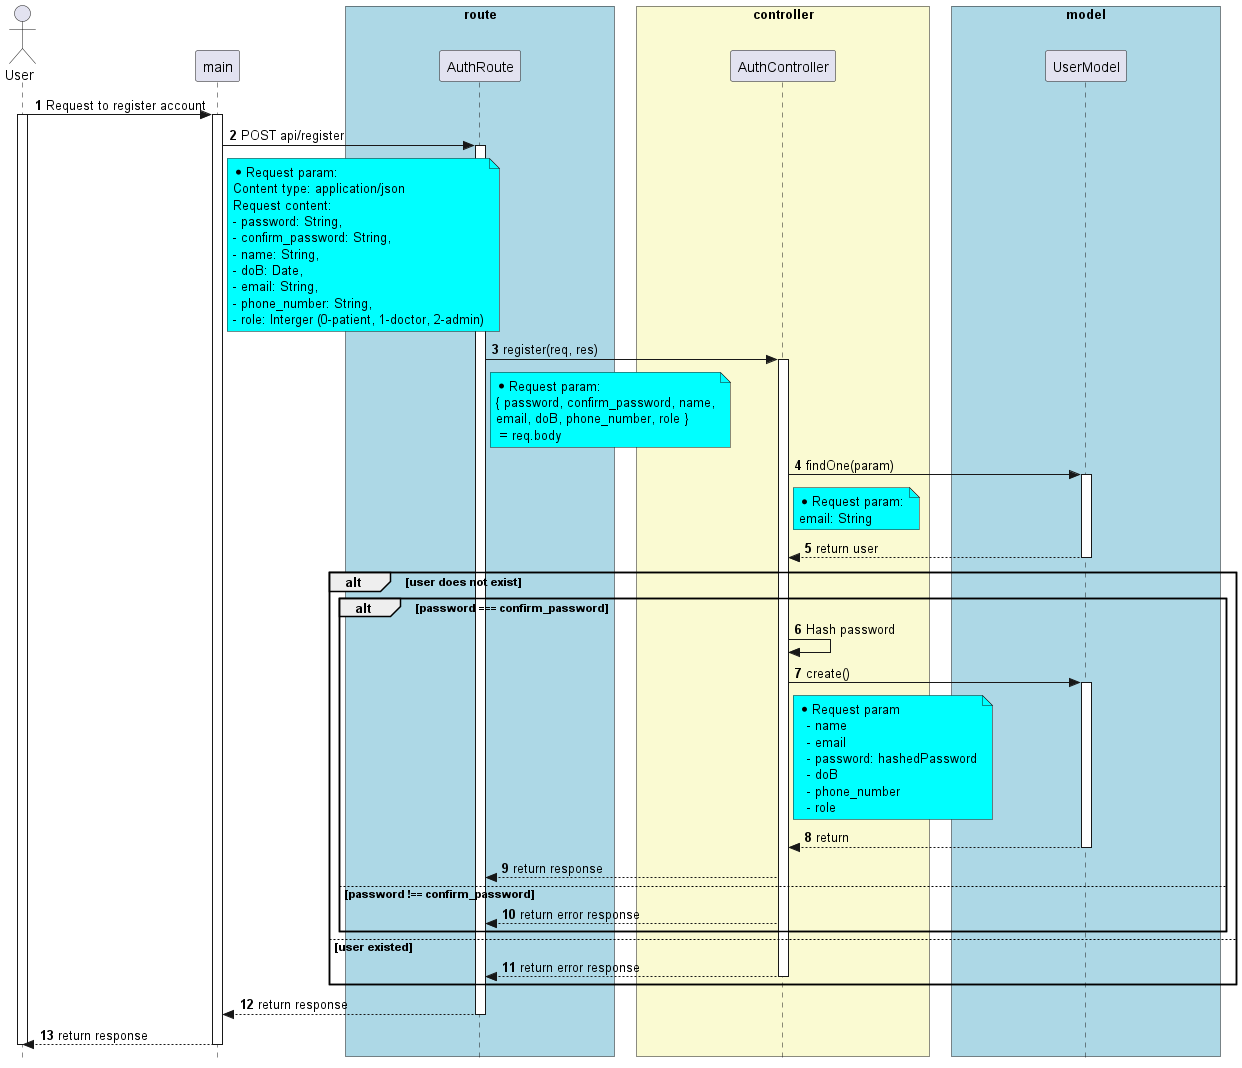
\includegraphics[width=16cm,height=12cm]{Images/server/sequence/server/register.png}
  \caption[Sơ đồ tuần tự cho API đăng ký tài khoản]{\bfseries \fontsize{12pt}{0pt}
  \selectfont Sơ đồ tuần tự cho API đăng ký tài khoản }
  \label{backend_register} %đặt tên cho ảnh
\end{figure}
Hình \ref{backend_register} mô tả quá trình đăng ký tài khoản trong ứng dụng. Người dùng gửi yêu cầu đăng ký, thông qua các tầng của hệ thống, yêu cầu này được xử lý bởi AuthController. Đầu tiên, hệ thống kiểm tra thông tin yêu cầu đăng ký, bao gồm việc kiểm tra mật khẩu và xác nhận mật khẩu có khớp hay không. Sau đó, AuthController kiểm tra xem người dùng đã tồn tại trong hệ thống hay chưa. Nếu người dùng chưa tồn tại và mật khẩu khớp, AuthController sẽ mã hóa mật khẩu và tạo một bản ghi mới trong UserModel để lưu thông tin đăng ký. Nếu người dùng đã tồn tại hoặc mật khẩu không khớp, hệ thống sẽ trả về response lỗi tương ứng. Sau khi xử lý, hệ thống trả về response kết quả cho người dùng.


\begin{figure}[H]
  \centering
  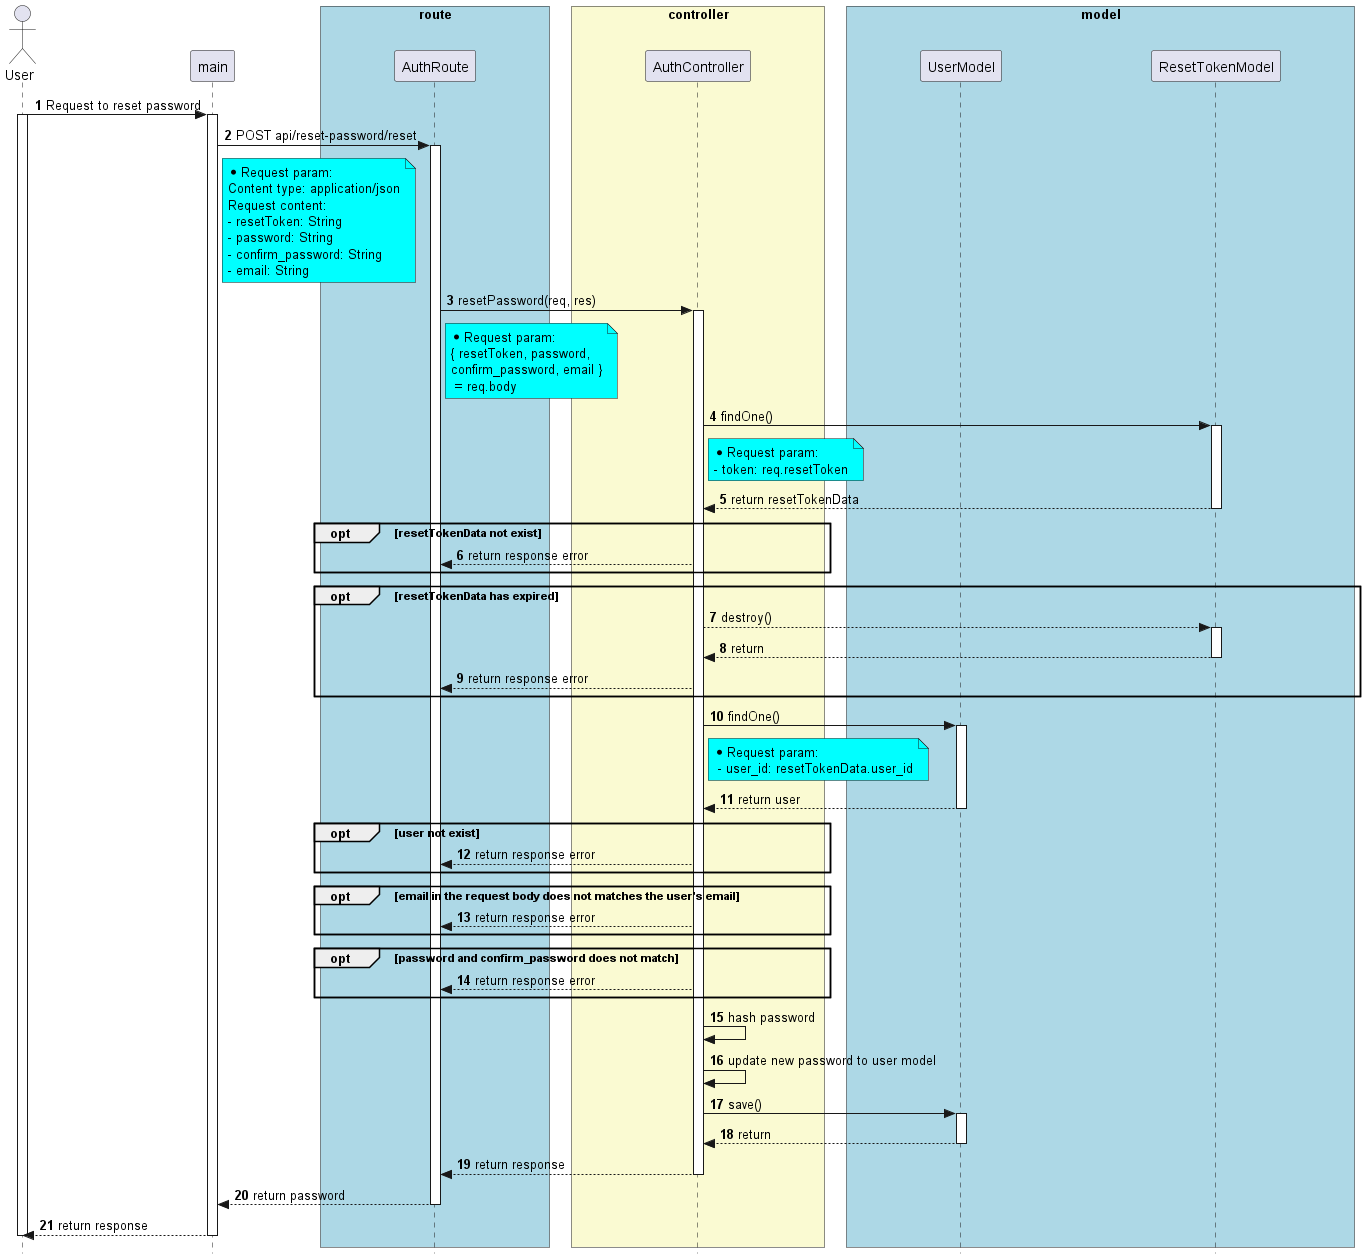
\includegraphics[width=16cm,height=13cm]{Images/server/sequence/server/resetPassword.png}
  \caption[Sơ đồ tuần tự cho API đăt lại mật khẩu ]{\bfseries \fontsize{12pt}{0pt}
  \selectfont Sơ đồ tuần tự cho API đăt lại mật khẩu }
  \label{resetPassword} %đặt tên cho ảnh
\end{figure}
Hình \ref{resetPassword} mô tả quá trình đặt lại mật khẩu (reset password) trong ứng dụng. Người dùng gửi yêu cầu đặt lại mật khẩu, thông qua các tầng của hệ thống, yêu cầu này được xử lý bởi AuthController. Đầu tiên, hệ thống kiểm tra thông tin yêu cầu đặt lại mật khẩu, bao gồm resetToken, mật khẩu mới và xác nhận mật khẩu. Sau đó, AuthController kiểm tra xem resetToken có hợp lệ hay không, bằng cách tìm kiếm trong ResetTokenModel. Nếu resetToken không hợp lệ hoặc đã hết hạn, hệ thống sẽ trả về response lỗi tương ứng. Nếu resetToken hợp lệ, AuthController tiếp tục kiểm tra xem người dùng có tồn tại và email trong yêu cầu có khớp với email của người dùng không. Nếu không hợp lệ, hệ thống sẽ trả về response lỗi tương ứng. Nếu mọi thông tin đều hợp lệ, AuthController sẽ mã hóa mật khẩu mới, cập nhật mật khẩu trong UserModel và trả về response thành công tới người dùng.

\begin{figure}[H]
  \centering
  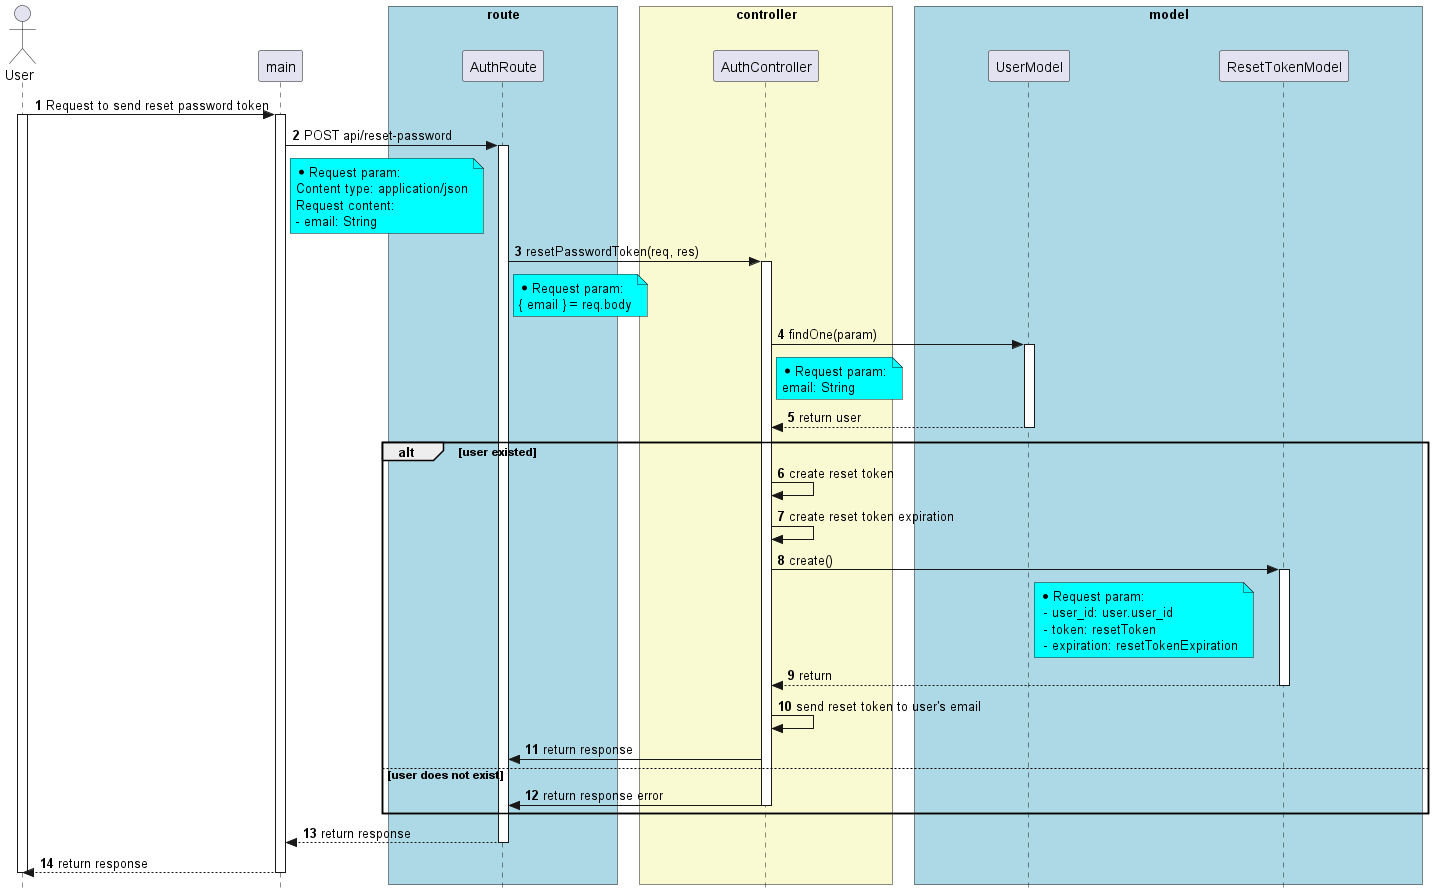
\includegraphics[width=16cm,height=9cm]{Images/server/sequence/server/resetPasswordToken.png}
  \caption[Sơ đồ tuần tự cho API gửi token đặt lại mật khẩu ]{\bfseries \fontsize{12pt}{0pt}
  \selectfont Sơ đồ tuần tự cho API gửi token đặt lại mật khẩu  }
  \label{resetPasswordToken} %đặt tên cho ảnh
\end{figure}
Hình \ref{resetPasswordToken} mô tả quá trình yêu cầu gửi mã thông báo đặt lại mật khẩu (reset password token) trong ứng dụng. Người dùng gửi yêu cầu đặt lại mật khẩu, thông qua các tầng của hệ thống, yêu cầu này được xử lý bởi AuthController. Đầu tiên, hệ thống kiểm tra thông tin yêu cầu đặt lại mật khẩu, bao gồm email người dùng. Sau đó, AuthController kiểm tra xem người dùng đã tồn tại trong hệ thống hay chưa. Nếu người dùng tồn tại, AuthController sẽ tạo một mã thông báo đặt lại mật khẩu (reset token) cùng với thời gian hết hạn cho mã (reset token expiration) và lưu thông tin này vào ResetTokenModel. Sau đó, hệ thống sẽ gửi mã thông báo đặt lại mật khẩu tới email của người dùng. Nếu người dùng không tồn tại, hệ thống sẽ trả về response lỗi tương ứng. Sau khi xử lý, hệ thống trả về response kết quả cho người dùng.

% ----------------------------------------------


% ------------------------News----------------------
\paragraph{API liên quan đến tin tức}
\mbox{}


\begin{figure}[H]
  \centering
  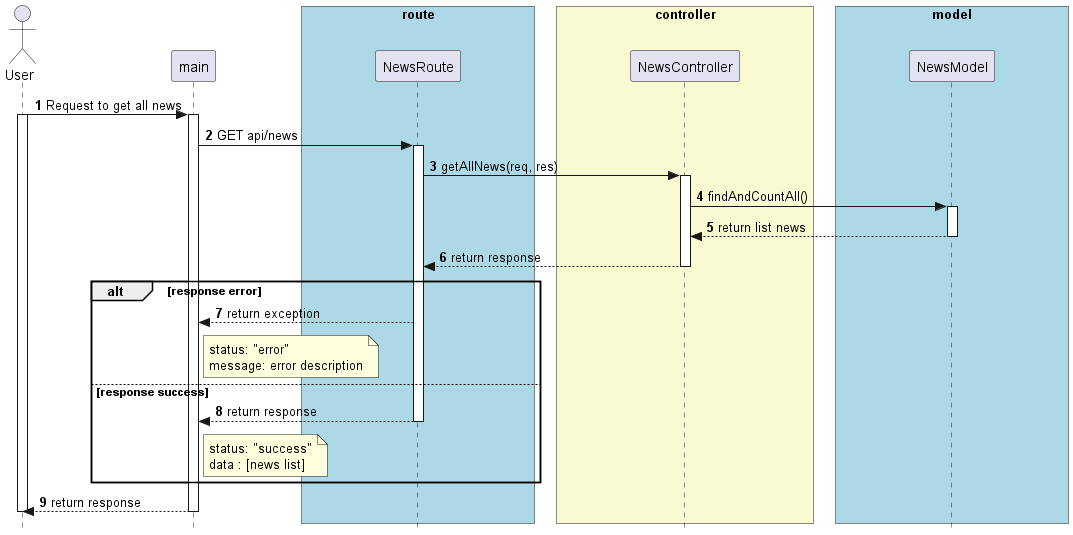
\includegraphics[width=16cm,height=9cm]{Images/server/sequence/server/getAllNews.png}
  \caption[Sơ đồ tuần tự cho API lấy tất cả thông tin của tin tức]{\bfseries \fontsize{12pt}{0pt}
  \selectfont Sơ đồ tuần tự cho API lấy tất cả thông tin của tin tức }
  \label{getAllNews} %đặt tên cho ảnh
\end{figure}
Hình \ref{getAllNews} mô tả quá trình lấy tất cả tin tức (news) trong ứng dụng. Người dùng gửi yêu cầu lấy tất cả tin tức, thông qua các tầng của hệ thống, yêu cầu này được xử lý bởi NewsController. NewsController tiếp tục truy vấn NewsModel để lấy danh sách tất cả các tin tức từ cơ sở dữ liệu. Sau đó, danh sách tin tức được trả về từ NewsModel và được gửi trở lại NewsRoute để trả về response cho người dùng. Nếu quá trình thực hiện thành công, hệ thống trả về response chứa danh sách tin tức cho người dùng. Nếu có lỗi xảy ra trong quá trình này, hệ thống trả về response lỗi với mô tả lỗi tương ứng. Sau khi xử lý, response cuối cùng được trả về tới người dùng.


\begin{figure}[H]
  \centering
  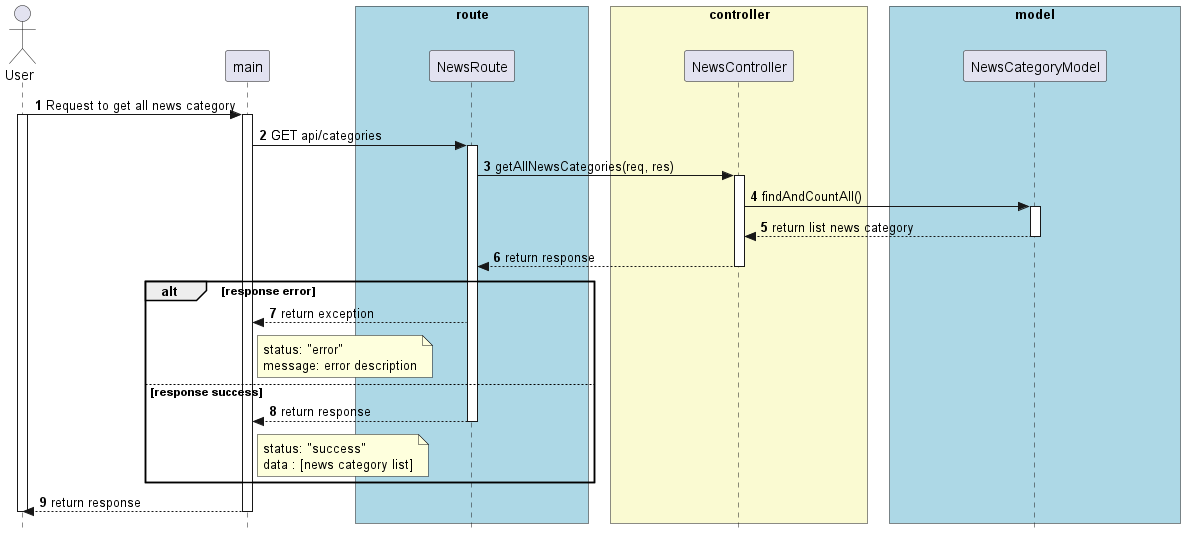
\includegraphics[width=16cm,height=9cm]{Images/server/sequence/server/getAllNewsCategories.png}
  \caption[Sơ đồ tuần tự cho API lấy tất cả thông tin của danh mục tin tức ]{\bfseries \fontsize{12pt}{0pt}
  \selectfont Sơ đồ tuần tự cho API lấy tất cả thông tin của danh mục tin tức }
  \label{getAllNewsCategories} %đặt tên cho ảnh
\end{figure}
Hình \ref{getAllNewsCategories} mô tả quá trình lấy tất cả danh mục tin tức (news category) trong ứng dụng. Người dùng gửi yêu cầu lấy tất cả danh mục tin tức, thông qua các tầng của hệ thống, yêu cầu này được xử lý bởi NewsController. NewsController tiếp tục truy vấn NewsCategoryModel để lấy danh sách tất cả các danh mục tin tức từ cơ sở dữ liệu. Sau đó, danh sách danh mục tin tức được trả về từ NewsCategoryModel và được gửi trở lại NewsRoute để trả về response cho người dùng. Nếu quá trình thực hiện thành công, hệ thống trả về response chứa danh sách danh mục tin tức cho người dùng. Nếu có lỗi xảy ra trong quá trình này, hệ thống trả về response lỗi với mô tả lỗi tương ứng. Sau khi xử lý, response cuối cùng được trả về tới người dùng.

\begin{figure}[H]
  \centering
  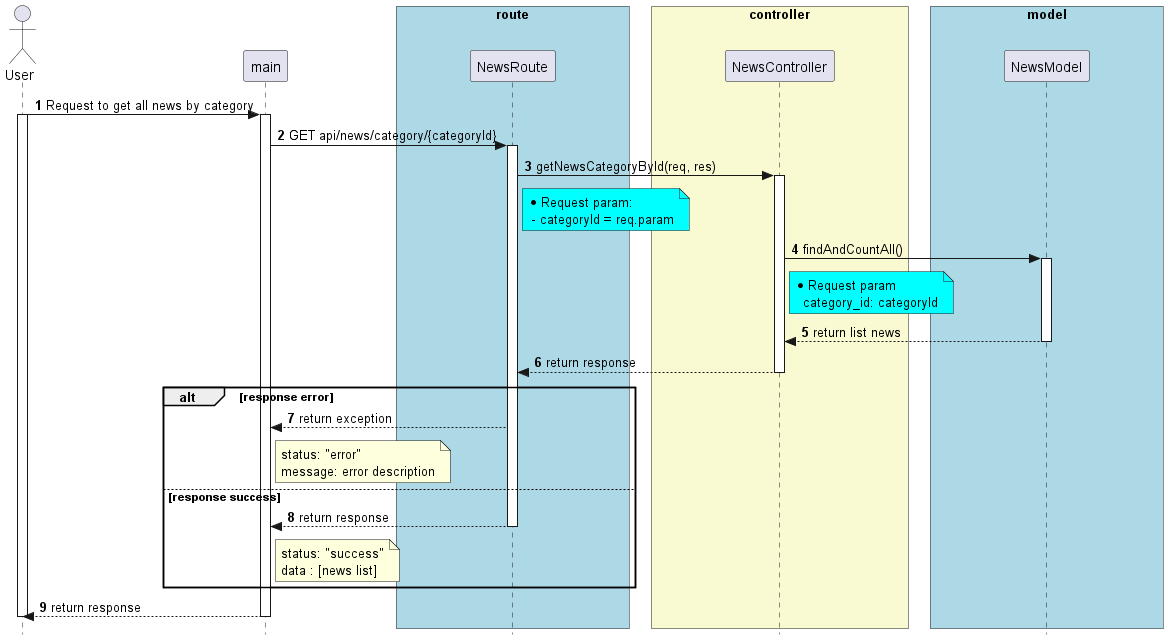
\includegraphics[width=16cm,height=9cm]{Images/server/sequence/server/getNewsByCategory.png}
  \caption[Sơ đồ tuần tự cho API lấy tất cả tin tức theo loại tin tức ]{\bfseries \fontsize{12pt}{0pt}
  \selectfont Sơ đồ tuần tự cho API lấy tất cả tin tức theo danh mục tin tức }
  \label{getNewsByCategory} %đặt tên cho ảnh
\end{figure}
Hình \ref{getNewsByCategory} mô tả quá trình lấy danh sách tin tức (news list) theo danh mục (category) trong ứng dụng. Người dùng gửi yêu cầu lấy danh sách tin tức theo danh mục, thông qua các tầng của hệ thống, yêu cầu này được xử lý bởi NewsController. NewsController tiếp tục truy vấn NewsModel để lấy danh sách tin tức dựa trên categoryId được truyền vào từ yêu cầu. Sau đó, danh sách tin tức được trả về từ NewsModel và được gửi trở lại NewsRoute để trả về response cho người dùng. Nếu quá trình thực hiện thành công, hệ thống trả về response chứa danh sách tin tức cho người dùng. Nếu có lỗi xảy ra trong quá trình này, hệ thống trả về response lỗi tương ứng. Sau khi xử lý, response cuối cùng được trả về tới người dùng.


\begin{figure}[H]
  \centering
  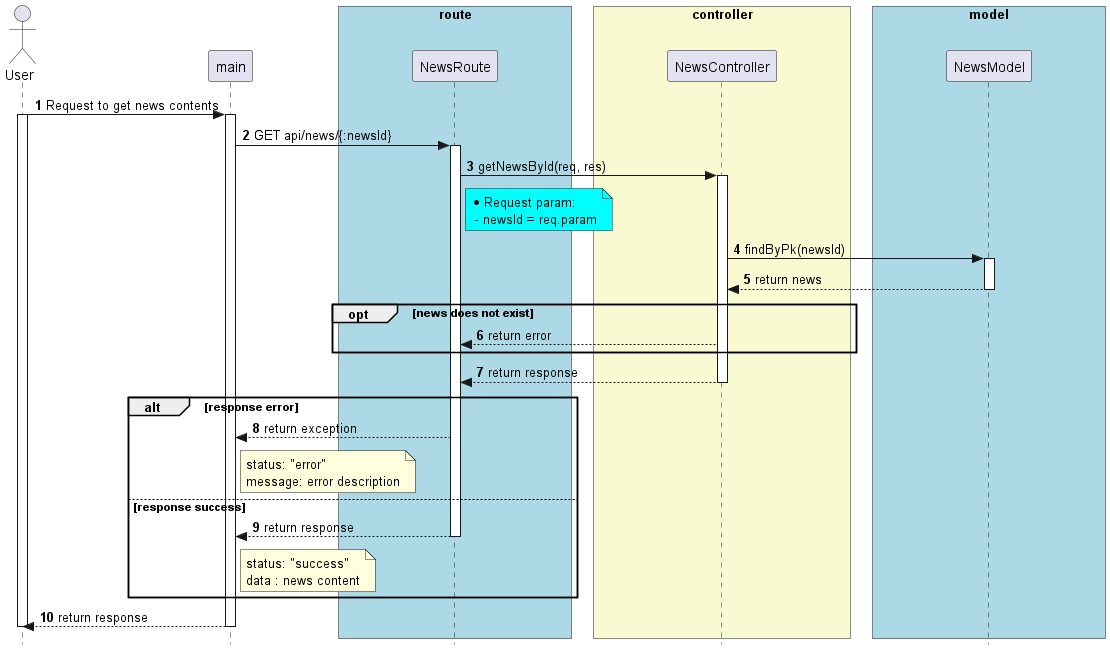
\includegraphics[width=16cm,height=9cm]{Images/server/sequence/server/getNewsById.png}
  \caption[Sơ đồ tuần tự cho API lấy nội dung của một tin tức ]{\bfseries \fontsize{12pt}{0pt}
  \selectfont Sơ đồ tuần tự cho API lấy nội dung của một tin tức }
  \label{getNewsById} %đặt tên cho ảnh
\end{figure}
Hình \ref{getNewsById} mô tả quá trình lấy nội dung tin tức (news content) trong ứng dụng. Người dùng gửi yêu cầu lấy nội dung tin tức, thông qua các tầng của hệ thống, yêu cầu này được xử lý bởi NewsController. NewsController tiếp tục truy vấn NewsModel để lấy nội dung tin tức dựa trên newsId được truyền vào từ yêu cầu. Sau đó, nội dung tin tức được trả về từ NewsModel và được gửi trở lại NewsRoute để trả về response cho người dùng. Nếu quá trình thực hiện thành công, hệ thống trả về response chứa nội dung tin tức cho người dùng. Nếu tin tức không tồn tại, hệ thống trả về response lỗi tương ứng. Nếu có lỗi xảy ra trong quá trình này, hệ thống trả về response lỗi với mô tả lỗi tương ứng. Sau khi xử lý, response cuối cùng được trả về tới người dùng.

\begin{figure}[H]
  \centering
  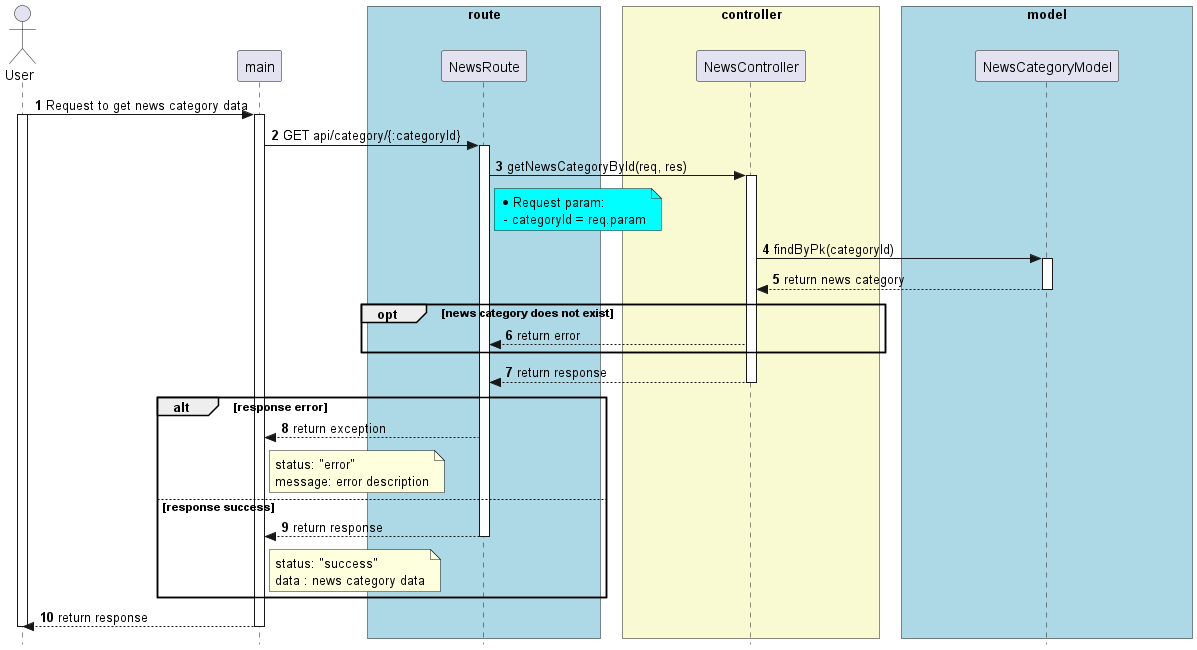
\includegraphics[width=16cm,height=9cm]{Images/server/sequence/server/getNewsCategoryById.png}
  \caption[Sơ đồ tuần tự cho API lấy thông tin của một danh mục tin tức ]{\bfseries \fontsize{12pt}{0pt}
  \selectfont Sơ đồ tuần tự cho API lấy thông tin của một danh mục tin tức }
  \label{getNewsCategoryById} %đặt tên cho ảnh
\end{figure}
Hình \ref{getNewsCategoryById} mô tả quá trình lấy dữ liệu danh mục tin tức (news category data) trong ứng dụng. Người dùng gửi yêu cầu lấy dữ liệu danh mục tin tức, thông qua các tầng của hệ thống, yêu cầu này được xử lý bởi NewsController. NewsController tiếp tục truy vấn NewsCategoryModel để lấy dữ liệu danh mục tin tức dựa trên categoryId được truyền vào từ yêu cầu. Sau đó, dữ liệu danh mục tin tức được trả về từ NewsCategoryModel và được gửi trở lại NewsRoute để trả về response cho người dùng. Nếu quá trình thực hiện thành công, hệ thống trả về response chứa dữ liệu danh mục tin tức cho người dùng. Nếu danh mục tin tức không tồn tại, hệ thống trả về response lỗi tương ứng. Nếu có lỗi xảy ra trong quá trình này, hệ thống trả về response lỗi với mô tả lỗi tương ứng. Sau khi xử lý, response cuối cùng được trả về tới người dùng.

% -----------------------------------------------------


% -------------------------ECG----------------------------
\paragraph{API liên quan đến bản ghi ECG}
\mbox{}



\begin{figure}[H]
  \centering
  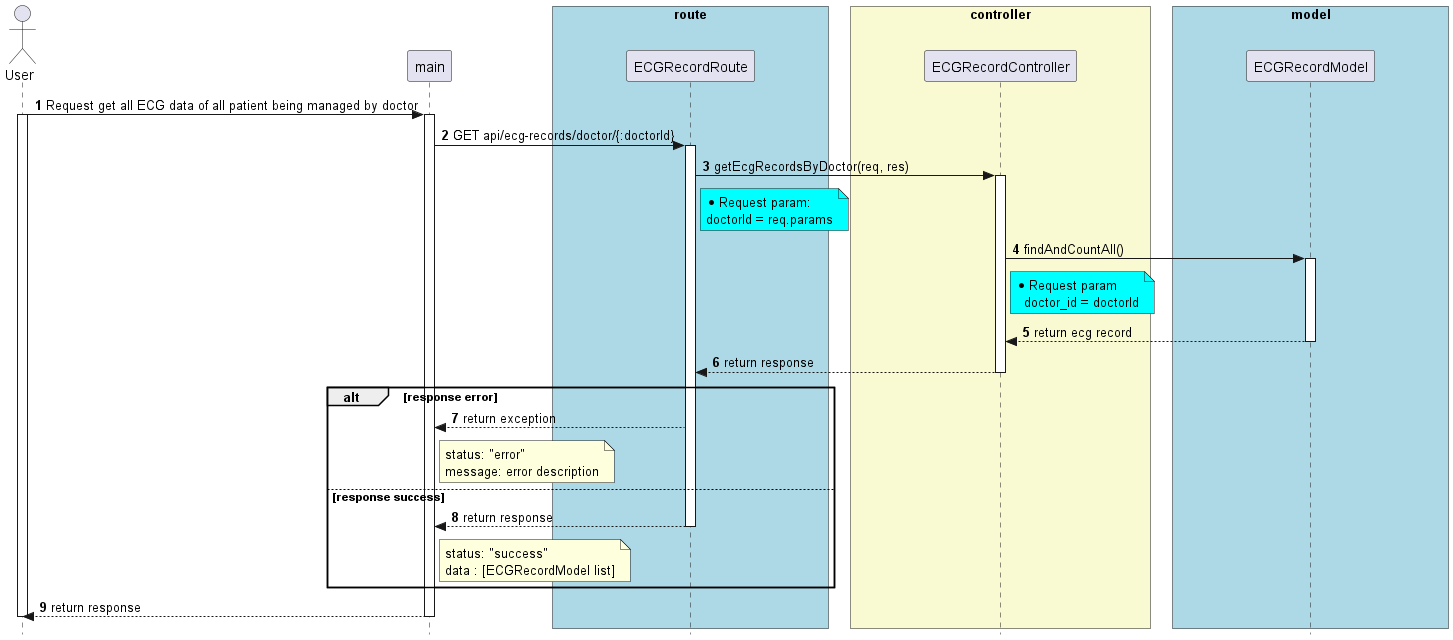
\includegraphics[width=16cm,height=9cm]{Images/server/sequence/server/getEcgRecordsByDoctor.png}
  \caption[Sơ đồ tuần tự cho API lấy thông tin phiên đo ECG của các bệnh nhân được quản lý bởi một bác sĩ ]{\bfseries \fontsize{12pt}{0pt}
  \selectfont Sơ đồ tuần tự cho API lấy thông tin phiên đo ECG của các bệnh nhân được quản lý bởi một bác sĩ }
  \label{getEcgRecordsByDoctor} %đặt tên cho ảnh
\end{figure}
Hình \ref{getEcgRecordsByDoctor} mô tả quá trình lấy dữ liệu ECG (Electrocardiogram) của tất cả bệnh nhân được quản lý bởi một bác sĩ trong ứng dụng. Người dùng (bác sĩ) gửi yêu cầu lấy dữ liệu ECG của tất cả bệnh nhân mà họ quản lý, thông qua các tầng của hệ thống, yêu cầu này được xử lý bởi ECGRecordController. ECGRecordController tiếp tục truy vấn ECGRecordModel để lấy dữ liệu ECG dựa trên doctorId (ID của bác sĩ) được truyền vào từ yêu cầu. Sau đó, danh sách dữ liệu ECG của các bệnh nhân được trả về từ ECGRecordModel và được gửi trở lại ECGRecordRoute để trả về response cho người dùng. Nếu quá trình thực hiện thành công, hệ thống trả về response chứa danh sách dữ liệu ECG cho bác sĩ. Nếu có lỗi xảy ra trong quá trình này, hệ thống trả về response lỗi tương ứng. Sau khi xử lý, response cuối cùng được trả về tới người dùng (bác sĩ).


\begin{figure}[H]
  \centering
  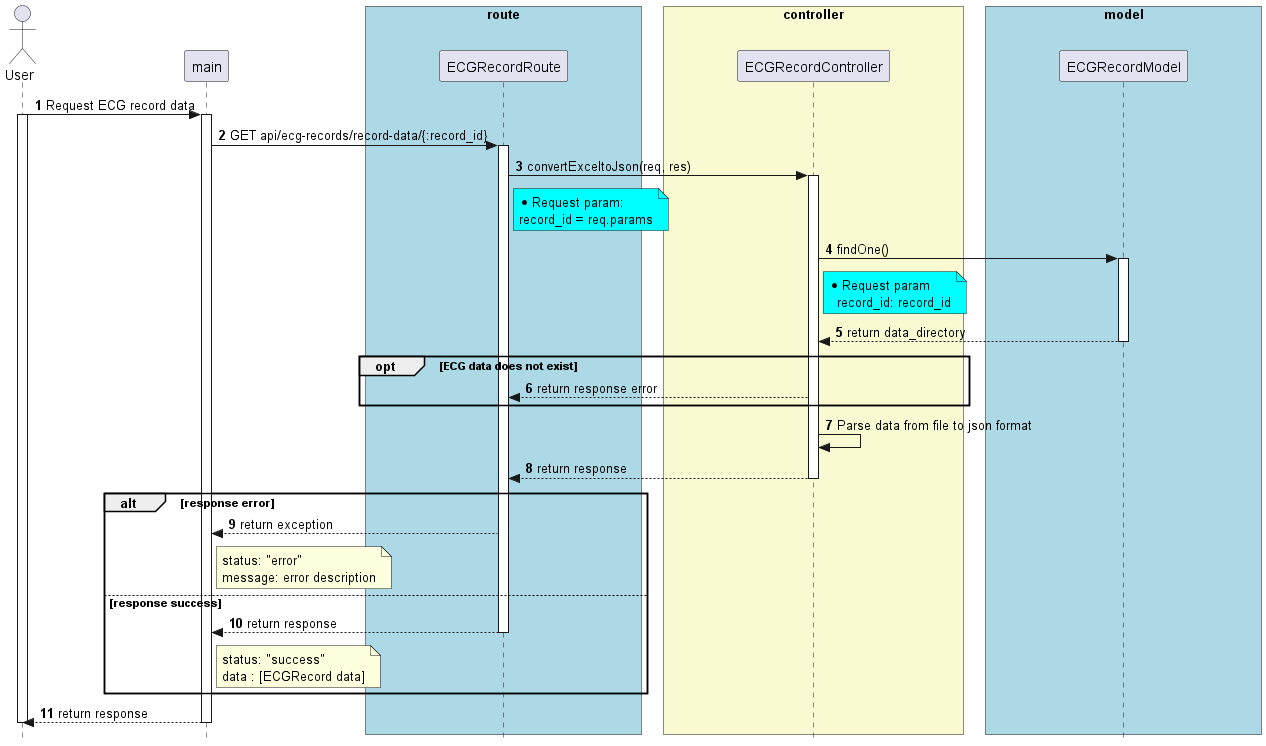
\includegraphics[width=16cm,height=9cm]{Images/server/sequence/server/convertExceltoJson.png}
  \caption[Sơ đồ tuần tự cho API lấy dữ liệu của một phiên đo ECG ]{\bfseries \fontsize{12pt}{0pt}
  \selectfont Sơ đồ tuần tự cho API lấy dữ liệu của một phiên đo ECG  }
  \label{convertExceltoJson} %đặt tên cho ảnh
\end{figure}
Hình \ref{convertExceltoJson} mô tả quá trình yêu cầu lấy dữ liệu ECG (Electrocardiogram) từ một bản ghi cụ thể trong ứng dụng. Người dùng (User) gửi yêu cầu lấy dữ liệu ECG cho một bản ghi có record\_id nhất định, thông qua các tầng của hệ thống, yêu cầu này được xử lý bởi ECGRecordController. ECGRecordController tiếp tục truy vấn ECGRecordModel để tìm kiếm bản ghi ECG dựa trên record\_id được truyền vào từ yêu cầu. Sau đó, data\_directory của bản ghi ECG được trả về từ ECGRecordModel và được gửi trở lại ECGRecordRoute để xử lý việc chuyển đổi dữ liệu từ định dạng file Excel sang định dạng JSON. Nếu quá trình thực hiện thành công, hệ thống trả về response chứa dữ liệu ECG của bản ghi tương ứng. Nếu có lỗi xảy ra trong quá trình này, hệ thống trả về response lỗi tương ứng. Sau khi xử lý, response cuối cùng được trả về tới người dùng.

\begin{figure}[H]
  \centering
  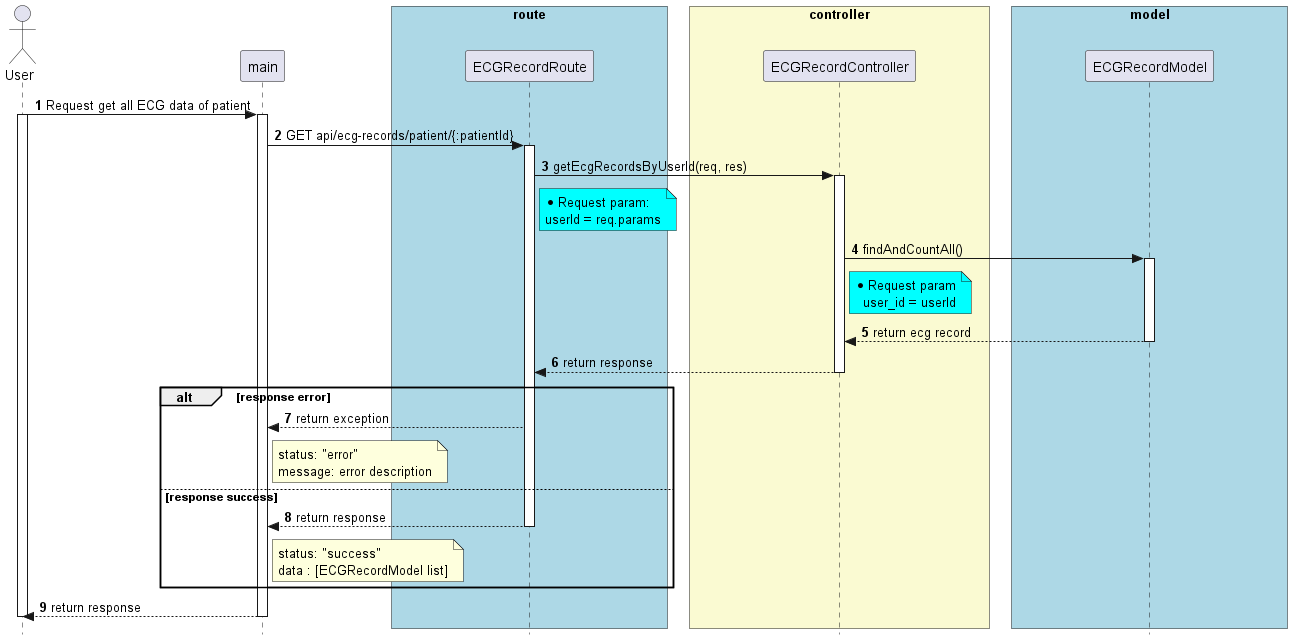
\includegraphics[width=16cm,height=9cm]{Images/server/sequence/server/getEcgRecordsByUserId.png}
  \caption[Sơ đồ tuần tự cho API lấy thông tin các phiên đo ECG của một bệnh nhân]{\bfseries \fontsize{12pt}{0pt}
  \selectfont Sơ đồ tuần tự cho API lấy thông tin các phiên đo ECG của một bệnh nhân }
  \label{getEcgRecordsByUserId} %đặt tên cho ảnh
\end{figure}
Hình \ref{getEcgRecordsByUserId} mô tả quá trình yêu cầu dữ liệu ECG (Electrocardiogram) của một bệnh nhân cụ thể từ ứng dụng. Người dùng (User) gửi yêu cầu lấy dữ liệu ECG cho một bệnh nhân với patientId nhất định, thông qua các tầng của hệ thống, yêu cầu này được xử lý bởi ECGRecordController. ECGRecordController tiếp tục truy vấn ECGRecordModel để tìm kiếm các bản ghi ECG của bệnh nhân dựa trên patientId được truyền vào từ yêu cầu. Sau đó, danh sách các bản ghi ECG của bệnh nhân được trả về từ ECGRecordModel và được gửi trở lại ECGRecordRoute để tạo response chứa danh sách này. Nếu quá trình thực hiện thành công, hệ thống trả về response chứa danh sách các bản ghi ECG của bệnh nhân tương ứng. Nếu có lỗi xảy ra trong quá trình này, hệ thống trả về response lỗi tương ứng. Sau khi xử lý, response cuối cùng được trả về tới người dùng.


\begin{figure}[H]
  \centering
  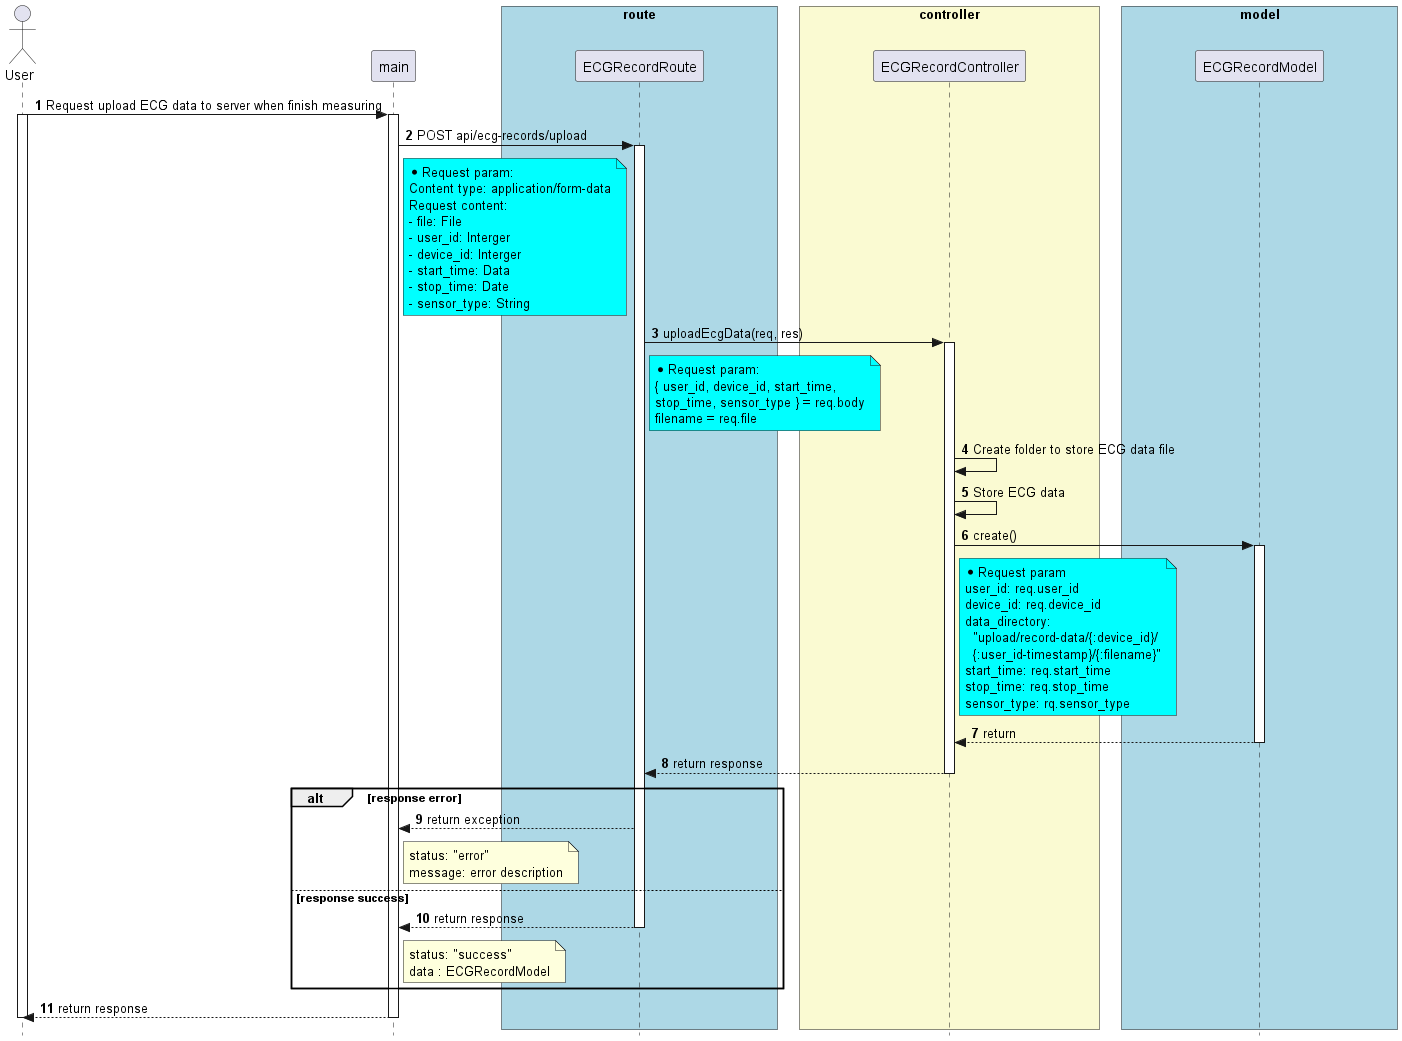
\includegraphics[width=16cm,height=13cm]{Images/server/sequence/server/uploadEcgData.png}
  \caption[Sơ đồ tuần tự cho API tải dữ liệu ECG lên server ]{\bfseries \fontsize{12pt}{0pt}
  \selectfont Sơ đồ tuần tự cho API tải dữ liệu ECG lên server }
  \label{uploadEcgData} %đặt tên cho ảnh
\end{figure}
Hình \ref{uploadEcgData} mô tả quá trình tải lên dữ liệu ECG (Electrocardiogram) sau khi hoàn thành việc đo đạc từ thiết bị đo ECG. Người dùng (User) gửi yêu cầu tải lên dữ liệu ECG cho một bệnh nhân cụ thể, thông qua các tầng của hệ thống, yêu cầu này được xử lý bởi ECGRecordController. ECGRecordController tiếp tục tạo folder mới để lưu trữ dữ liệu ECG, sau đó lưu dữ liệu ECG được tải lên vào folder vừa tạo. Tiếp theo, ECGRecordController tạo một bản ghi mới trong ECGRecordModel, lưu trữ thông tin về người dùng (user\_id), thiết bị đo (device\_id), thời gian bắt đầu đo (start\_time), thời gian kết thúc đo (stop\_time), loại cảm biến (sensor\_type) và đường dẫn của dữ liệu ECG được lưu trữ. Sau đó, ECGRecordModel trả về thông tin vừa lưu vào ECGRecordController. Nếu quá trình tải lên thành công, hệ thống trả về response thành công chứa thông tin về bản ghi ECG vừa tạo. Nếu có lỗi xảy ra trong quá trình này, hệ thống trả về response lỗi tương ứng. Sau khi xử lý, response cuối cùng được trả về tới người dùng.
% -----------------------------------------------------



% -----------------------PatientDoctor------------------------------
\paragraph{API liên quan liên quan đến việc phân công bệnh nhân cho bác sỹ}
\mbox{}


\begin{figure}[H]
  \centering
  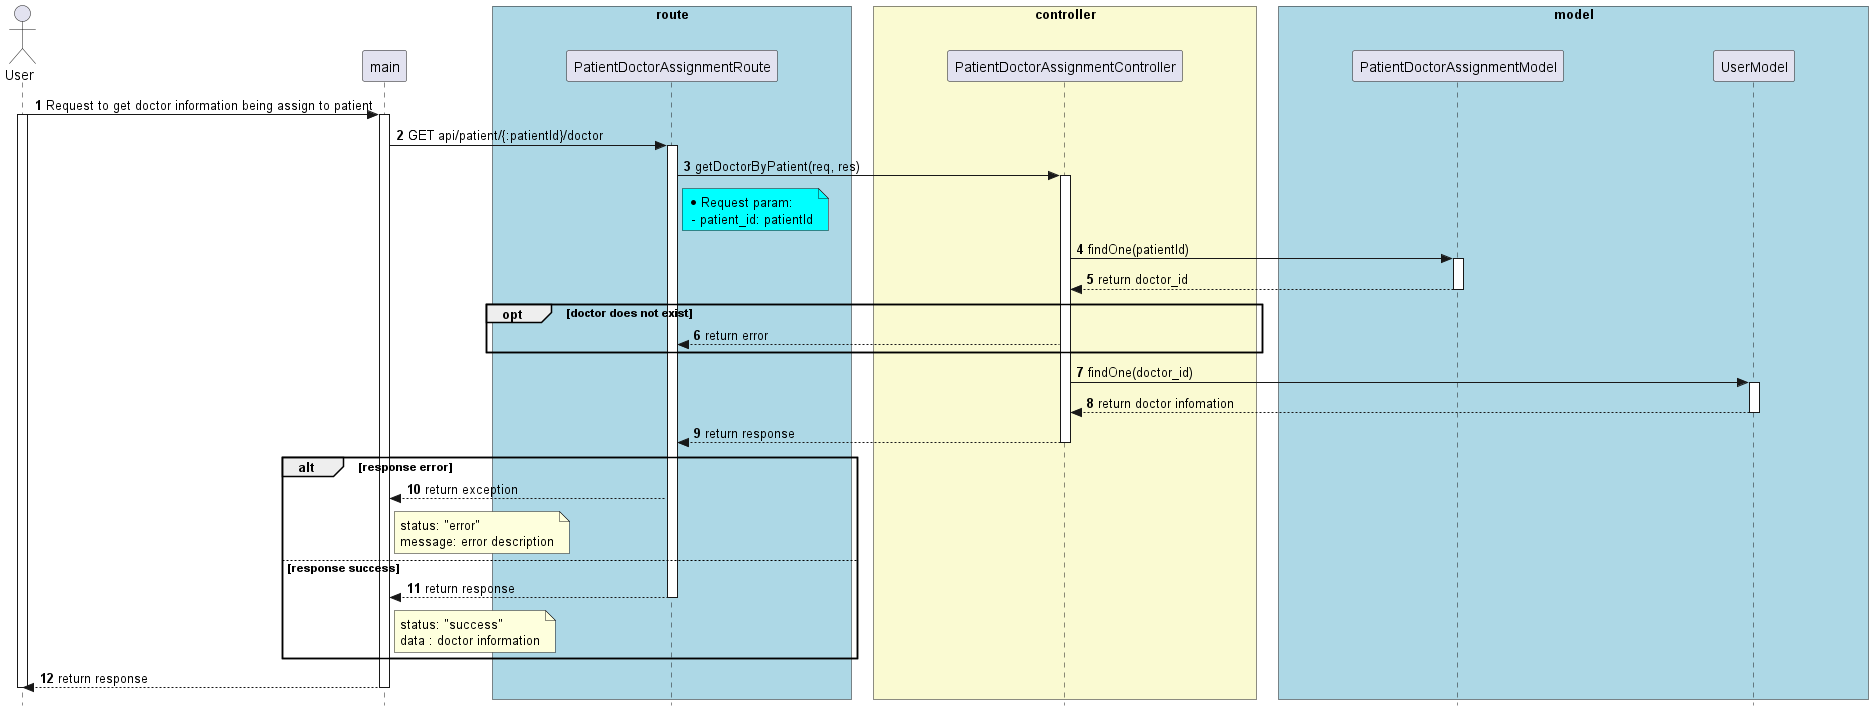
\includegraphics[width=16cm,height=10cm]{Images/server/sequence/server/getDoctorByPatient.png}
  \caption[Sơ đồ tuần tự cho API lấy thông tin bác sĩ được phân công cho một bệnh nhân ]{\bfseries \fontsize{12pt}{0pt}
  \selectfont Sơ đồ tuần tự cho API lấy thông tin bác sĩ được phân công cho một bệnh nhân }
  \label{getDoctorByPatient} %đặt tên cho ảnh
\end{figure}
Hình \ref{getDoctorByPatient} mô tả quá trình lấy thông tin bác sĩ được phân công cho một bệnh nhân cụ thể. Người dùng (User) gửi yêu cầu lấy thông tin bác sĩ của một bệnh nhân cụ thể, thông qua các tầng của hệ thống, yêu cầu này được xử lý bởi PatientDoctorAssignmentController. PatientDoctorAssignmentController tìm kiếm thông tin liên kết giữa bệnh nhân và bác sĩ trong PatientDoctorAssignmentModel bằng cách tìm bản ghi với patient\_id trùng khớp với bệnh nhân được chỉ định. Nếu không tìm thấy thông tin liên kết, hệ thống trả về response lỗi tương ứng. Nếu tìm thấy thông tin liên kết, PatientDoctorAssignmentController sẽ tiếp tục tìm kiếm thông tin của bác sĩ trong UserModel bằng cách sử dụng doctor\_id lấy từ bản ghi liên kết. Sau khi tìm thấy thông tin của bác sĩ, hệ thống trả về response thành công chứa thông tin về bác sĩ đó. Nếu có lỗi xảy ra trong quá trình này, hệ thống trả về response lỗi tương ứng. Sau khi xử lý, response cuối cùng được trả về tới người dùng.


\begin{figure}[H]
  \centering
  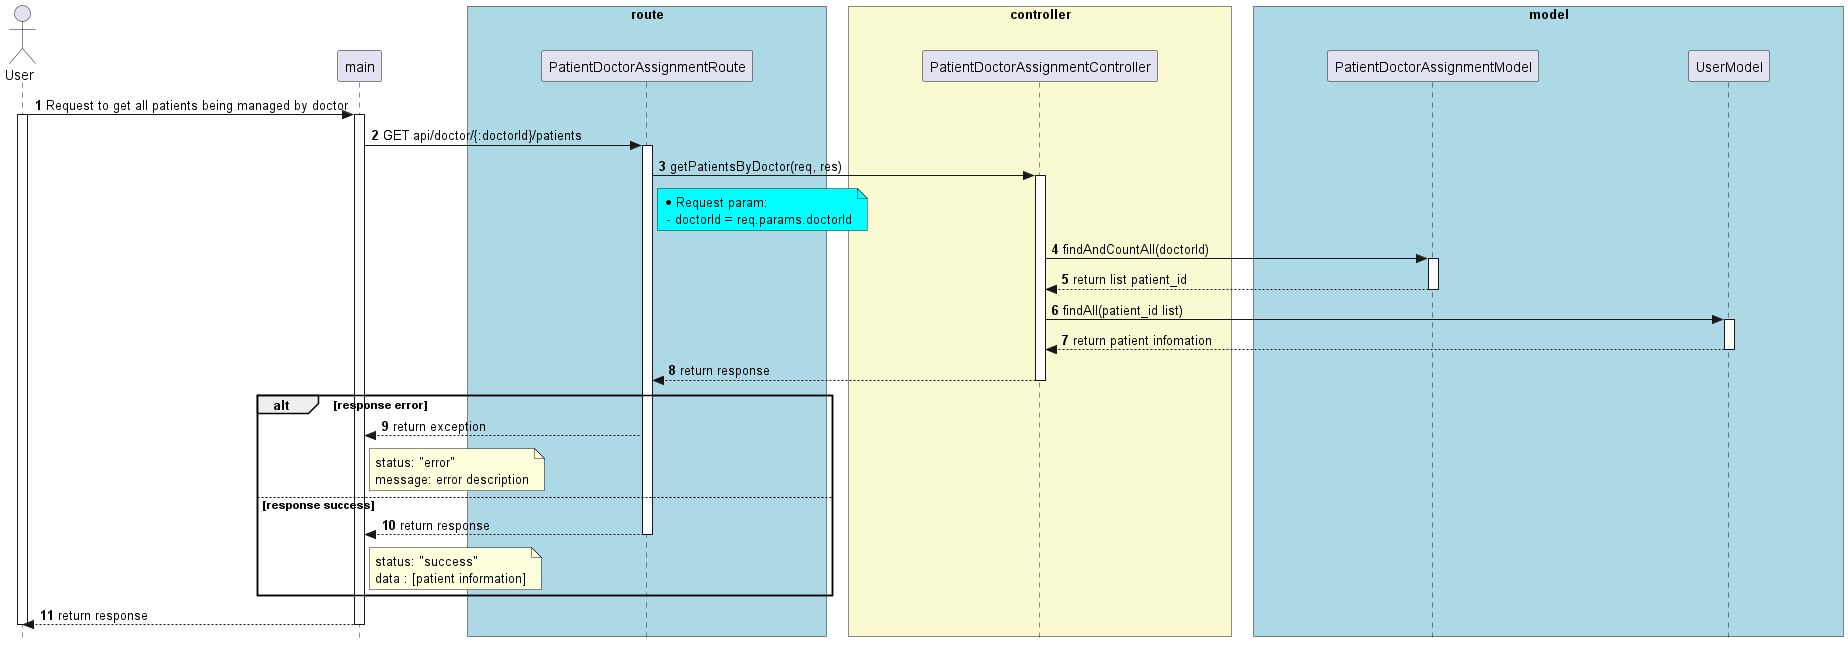
\includegraphics[width=16cm,height=9cm]{Images/server/sequence/server/getPatientsByDoctor.png}
  \caption[Sơ đồ tuần tự cho API lấy thông tin tất cả bệnh nhân được quản lý bởi một bác sĩ]{\bfseries \fontsize{12pt}{0pt}
  \selectfont Sơ đồ tuần tự cho API lấy thông tin tất cả bệnh nhân được quản lý bởi một bác sĩ }
  \label{getPatientsByDoctor} %đặt tên cho ảnh
\end{figure}
Hình \ref{getPatientsByDoctor}  mô tả quá trình lấy thông tin tất cả bệnh nhân được quản lý bởi một bác sĩ cụ thể. Người dùng (User) gửi yêu cầu lấy thông tin tất cả bệnh nhân của một bác sĩ cụ thể, thông qua các tầng của hệ thống, yêu cầu này được xử lý bởi PatientDoctorAssignmentController. PatientDoctorAssignmentController tìm kiếm thông tin liên kết giữa bác sĩ và bệnh nhân trong PatientDoctorAssignmentModel bằng cách tìm bản ghi với doctorId trùng khớp với bác sĩ được chỉ định. Sau đó, PatientDoctorAssignmentController tìm kiếm thông tin của tất cả bệnh nhân có trong danh sách patient\_id tìm thấy, thông qua UserModel. Mỗi bệnh nhân sẽ có thông tin riêng bao gồm tên, tuổi, địa chỉ, v.v. Sau khi tìm thấy thông tin của tất cả bệnh nhân, hệ thống trả về response thành công chứa danh sách thông tin của các bệnh nhân đó. Nếu có lỗi xảy ra trong quá trình này, hệ thống trả về response lỗi tương ứng. Sau khi xử lý, response cuối cùng được trả về tới người dùng.

% -----------------------------------------------------


\paragraph{Web}
\mbox{}


\begin{figure}[H]
  \centering
  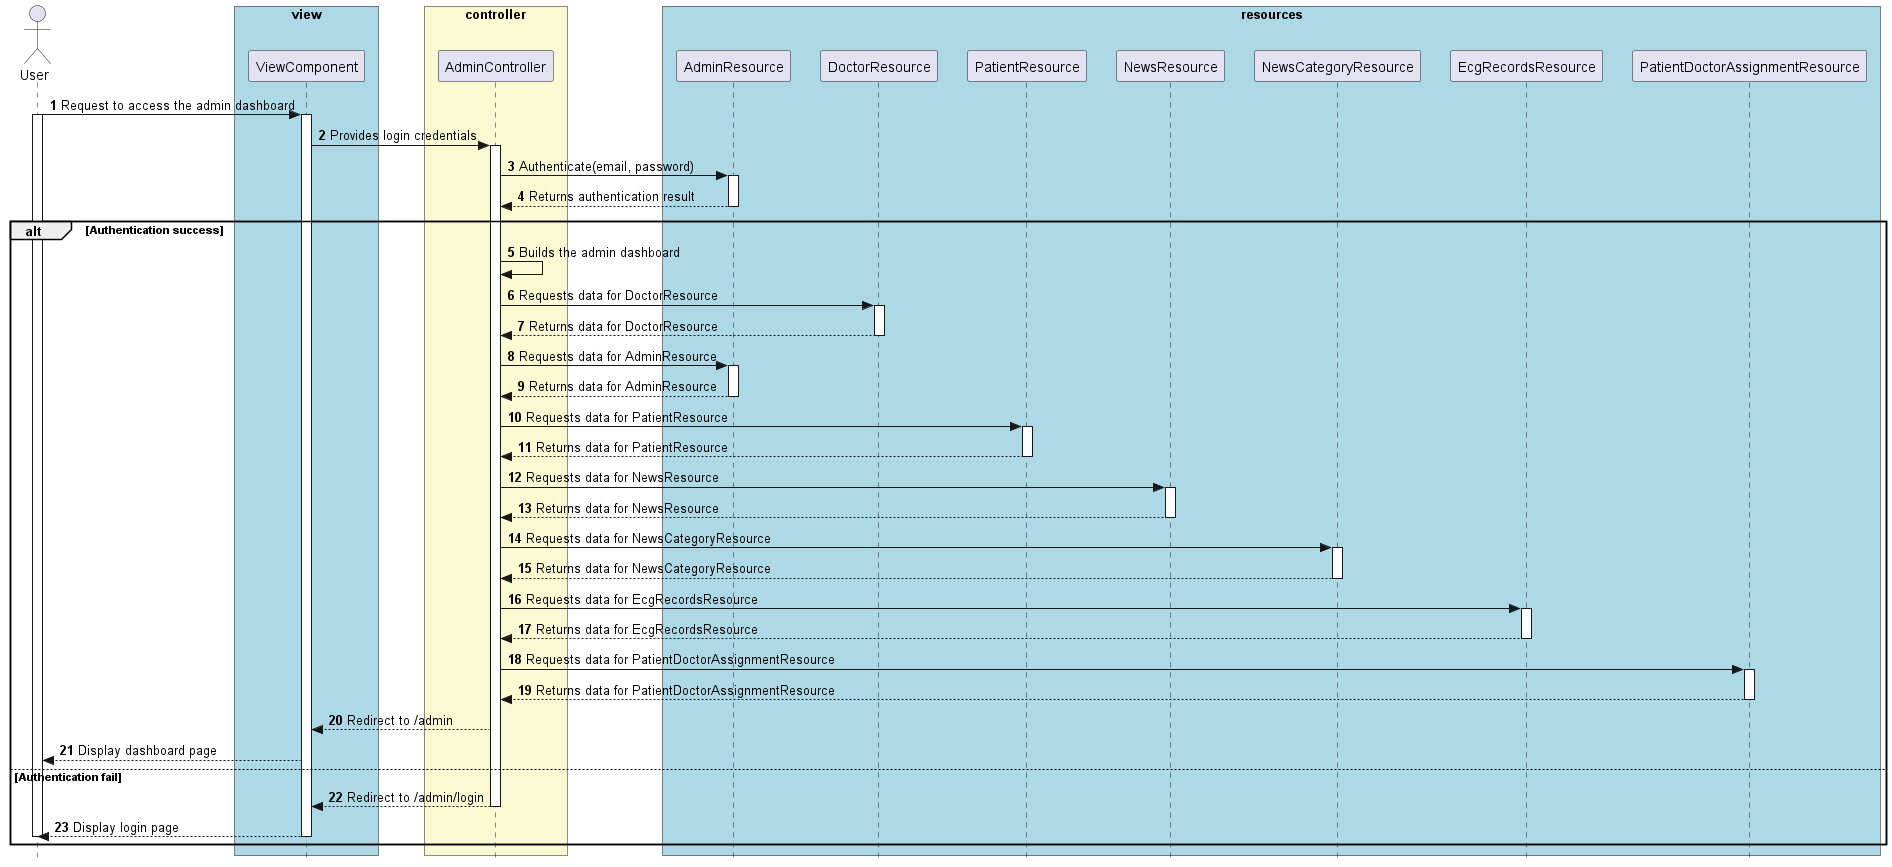
\includegraphics[width=16cm,height=10cm]{Images/server/sequence/web/seq_auth.png}
  \caption[Sơ đồ tuần tự cho quá trình truy cập vào trang quản trị (admin dashboard) ]{\bfseries \fontsize{12pt}{0pt}
  \selectfont Sơ đồ tuần tự cho quá trình truy cập vào trang quản trị (admin dashboard) }
  \label{seq_auth} %đặt tên cho ảnh
\end{figure}
Hình \ref{seq_auth} mô tả quá trình truy cập vào bảng điều khiển quản trị (admin dashboard) của người dùng (User). Khi người dùng yêu cầu truy cập vào admin dashboard, hệ thống sẽ yêu cầu xác thực thông qua ViewComponent. Nếu xác thực thành công, AdminJS sẽ xây dựng admin dashboard và yêu cầu dữ liệu từ các tài nguyên (resources) khác nhau để hiển thị thông tin.



Nếu xác thực thành công, AdminJS sẽ yêu cầu dữ liệu từ các tài nguyên khác nhau, bao gồm DoctorResource, AdminResource, PatientResource, NewsResource, NewsCategoryResource, EcgRecordsResource và PatientDoctorAssignmentResource. Mỗi tài nguyên sẽ trả về dữ liệu tương ứng và AdminJS sẽ sử dụng các dữ liệu này để hiển thị trên admin dashboard.



Sau khi AdminJS đã thu thập đủ dữ liệu từ các tài nguyên, nó sẽ chuyển hướng ViewComponent đến trang /admin để hiển thị admin dashboard cho người dùng. Nếu xác thực không thành công, AdminJS sẽ chuyển hướng ViewComponent đến trang /admin/login để hiển thị trang đăng nhập cho người dùng.



Sau khi hoàn tất, hệ thống sẽ trả về response cuối cùng và hiển thị trang tương ứng cho người dùng.


\begin{figure}[H]
  \centering
  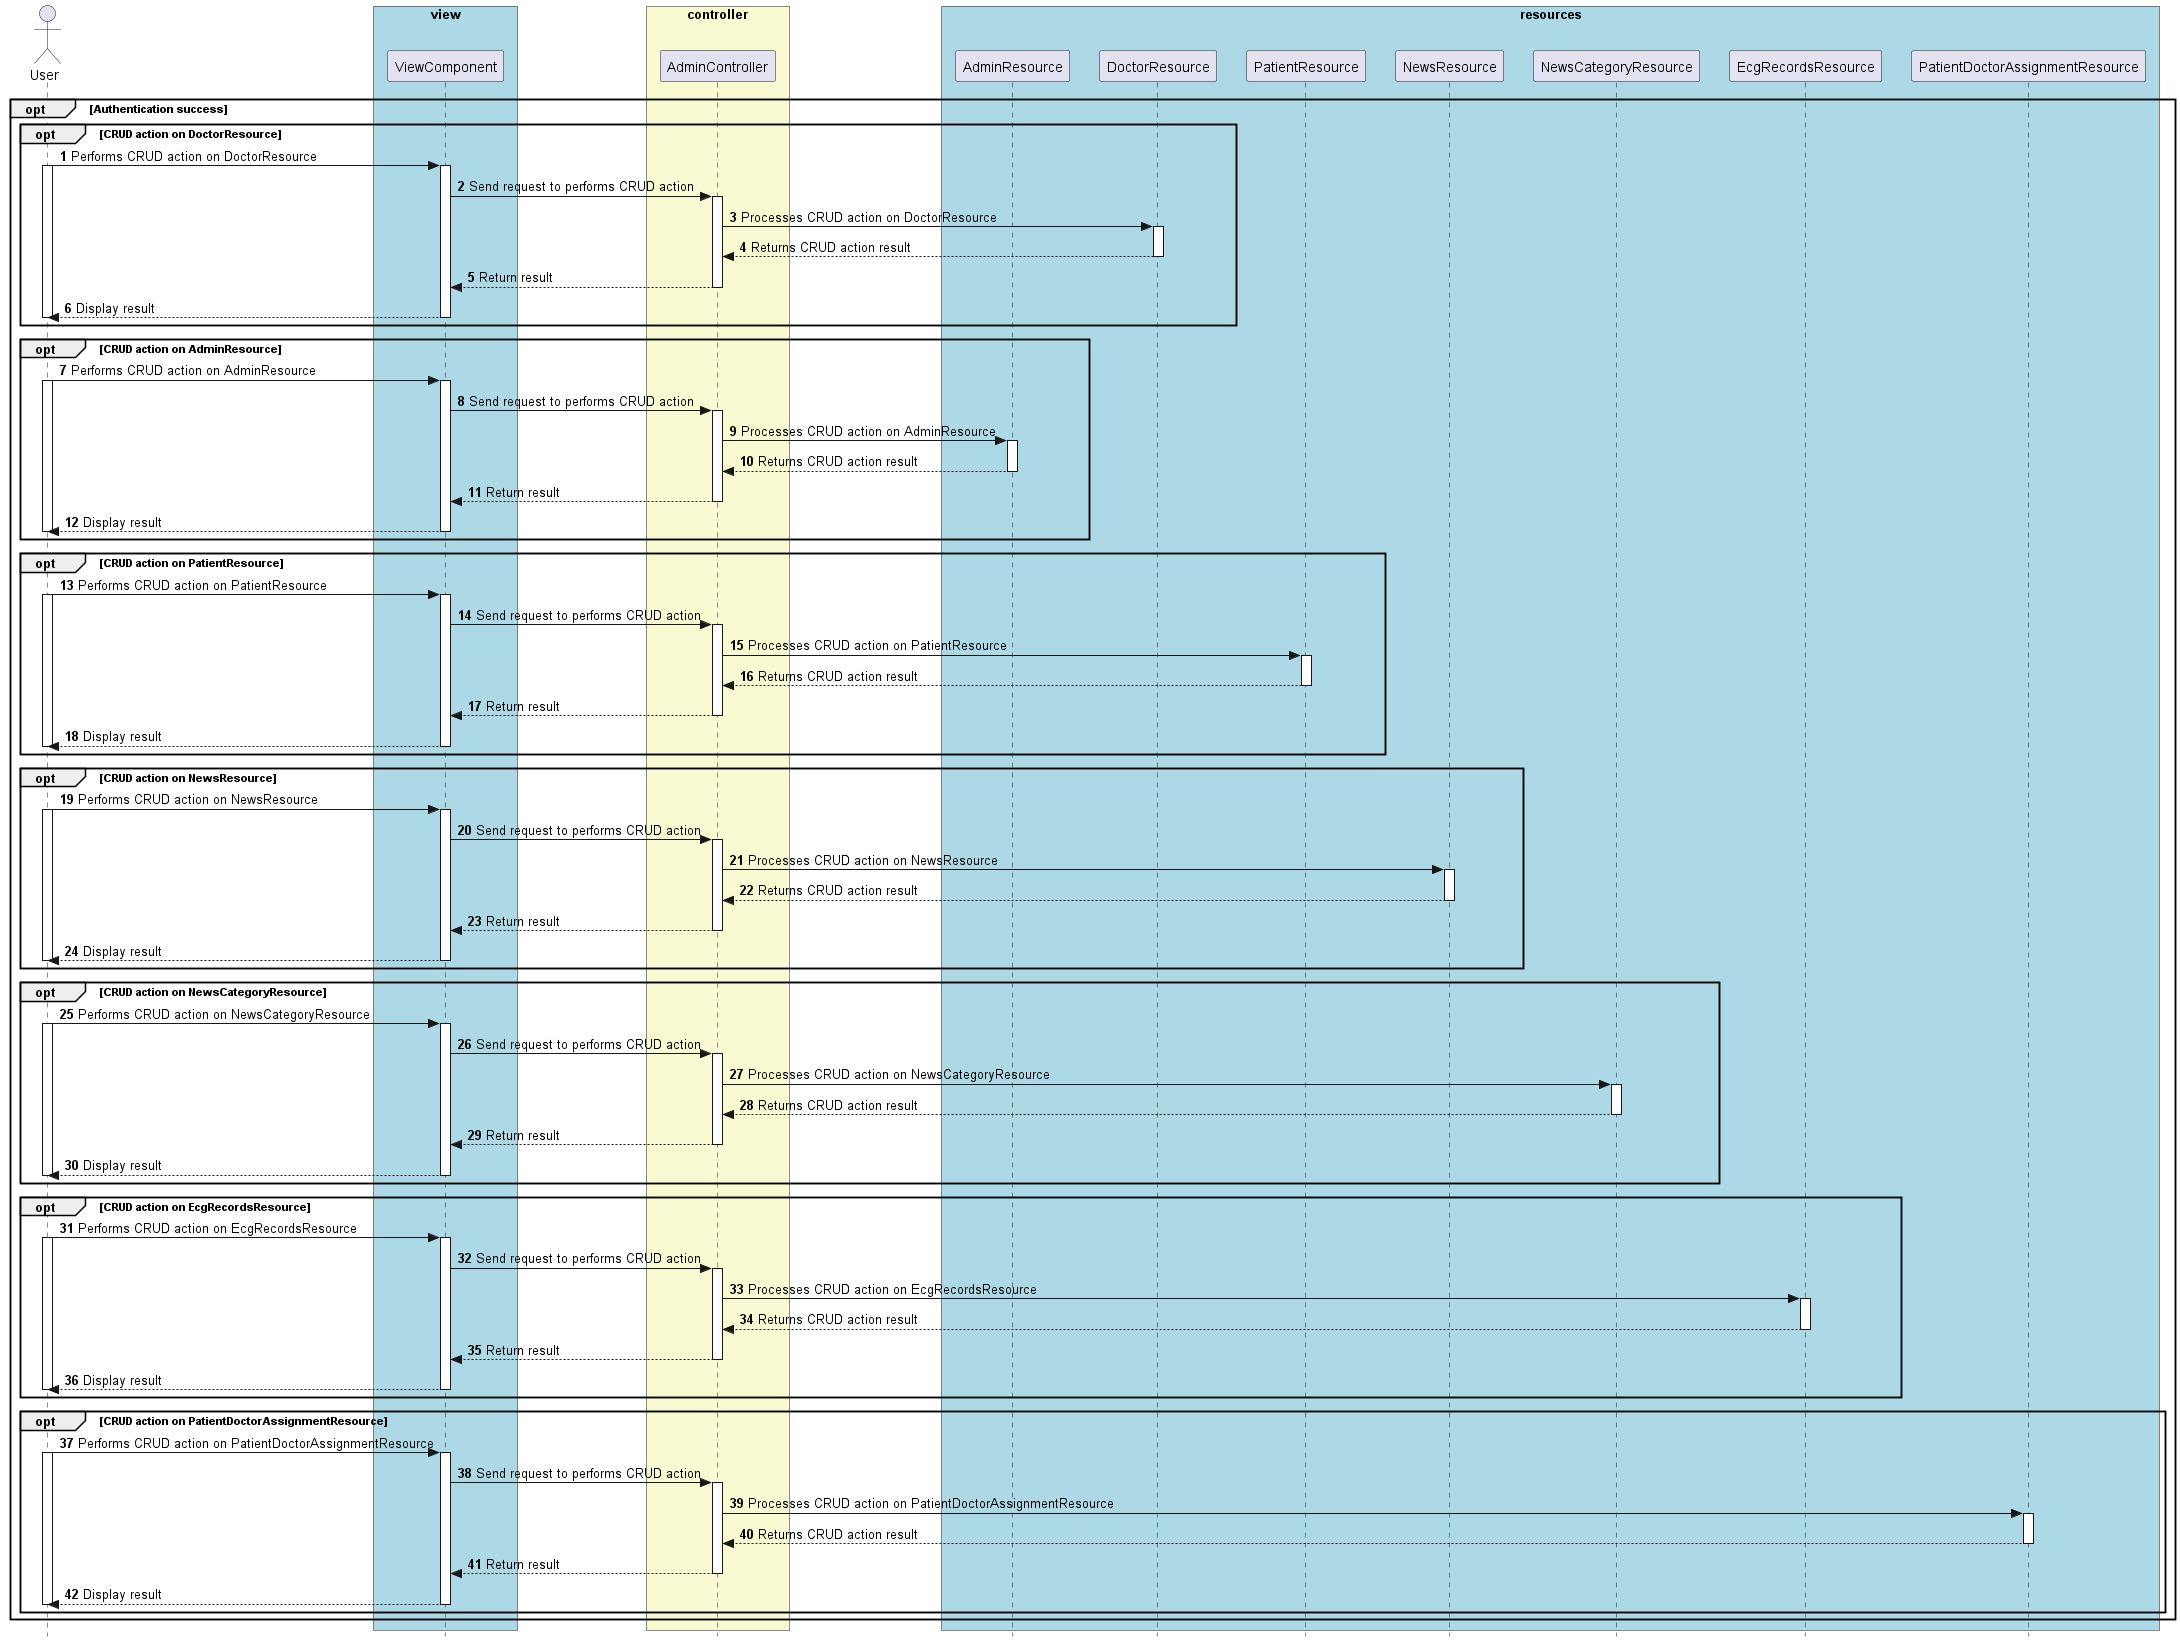
\includegraphics[width=16cm,height=14cm]{Images/server/sequence/web/seq_crud.png}
  \caption[Sơ đồ tuần tự cho quá trình trình thực hiện các thao tác CRUD trên các tài nguyên (resources) ]{\bfseries \fontsize{12pt}{0pt}
  \selectfont Sơ đồ tuần tự cho quá trình trình thực hiện các thao tác CRUD trên các tài nguyên (resources) }
  \label{seq_crud} %đặt tên cho ảnh
\end{figure}
Hình \ref{seq_crud}  mô tả quá trình thực hiện các thao tác CRUD trên các tài nguyên (resources) khác nhau của admin dashboard khi người dùng (User) thực hiện các thao tác trong ViewComponent.


Khi người dùng thực hiện các thao tác CRUD trên các tài nguyên, hệ thống sẽ xác thực người dùng trước đó. Sau khi xác thực thành công, người dùng sẽ thực hiện các thao tác CRUD trên ViewComponent, và ViewComponent sẽ gửi yêu cầu thực hiện thao tác tương ứng tới AdminJS.


Sau đó, AdminJS sẽ thực hiện thao tác CRUD tương ứng trên các tài nguyên, bao gồm DoctorResource, AdminResource, PatientResource, NewsResource, NewsCategoryResource, EcgRecordsResource và PatientDoctorAssignmentResource. Mỗi tài nguyên sẽ xử lý yêu cầu và trả về kết quả tương ứng cho AdminJS.


Sau khi AdminJS đã nhận được kết quả từ các tài nguyên, nó sẽ trả về kết quả đó cho ViewComponent. ViewComponent sẽ hiển thị kết quả tương ứng cho người dùng. Quá trình này được thực hiện đối với từng tài nguyên mà người dùng yêu cầu thực hiện thao tác CRUD.

\newpage